\documentclass[12pt]{article}

% double-spacing
\usepackage{setspace}
\doublespacing

%% line numbers
%% (turn on before submission)
%\usepackage{lineno}
%\linenumbers

% 1 inch margins
\usepackage[margin=1in]{geometry}

% text color
\usepackage{xcolor}

% bold symbols
\usepackage{bm}

% matrices
\usepackage{amsmath}

% proof environment
\usepackage{amsthm}

% images
\usepackage{graphicx}

% links
\usepackage{hyperref}

% highlight text that needs editing in red
\newcommand{\edit}[1]{{\color{red}{#1}}}
\newcommand{\add}[1]{{\color{red}{[... #1 ...]}}}

% bibliography
\usepackage[super]{natbib} % superscripts
\renewcommand{\refname}{} % empty title
\setcitestyle{citesep={,}} % comma separated
\renewcommand\bibname{Supplemental References} % change title

% add "S" before section numbers and figure numbers
\renewcommand{\thesection}{S\arabic{section}}
%\renewcommand{\thesubsection}{S\arabic{subsection}}
\renewcommand{\thefigure}{S\arabic{figure}}

% add lists of figures to TOC
\usepackage[nottoc]{tocbibind}
\renewcommand{\listfigurename}{List of Supplemental Figures} % change title

% keep figures in section
\usepackage[section]{placeins}


%\newcommand{\supplementarysection}{%
%  \setcounter{figure}{0}% Reset figure counter
%  \let\oldthefigure\thefigure% Capture figure numbering scheme
%  \renewcommand{\thefigure}{S\oldthefigure}% Prefix figure number with S
%  \section{Supplementary section}% Set supplementary section
%  %\let\oldchapter\chapter% Copy \chapter into \oldchapter
%  %\renewcommand{\chapter}{% Update \chapter
%  %  \let\thefigure\oldthefigure% Copy \thefigure into \oldthefigure
%   % \let\chapter\oldchapter% Restore original \chapter
%   % \oldchapter% Call original \chapter
%  %}
%}

% reference across files
\usepackage{xr}
\externaldocument{SpuriousAssociations}



%% title
\title{Supplemental Information}




\begin{document}

\maketitle
\tableofcontents % need to fix numbering

\newpage
\listoffigures

\newpage
%\listoftables

%\supplementarysection

\newpage
\section{Comparison of PCs and Model-Based Admixture Proportions}
\label{sec:pcsvspi}

In many African American populations, only one principal component may be needed to capture ancestral heterogeneity, at least with respect to differences in the relative proportion of African and European continental ancestry.
We investigated whether this statement holds true in three samples of African American individuals from the Women's Health Initiative SNP Health Association Resource (WHI SHARe) and two Trans-Omics for Precision Medicine (TOPMed) contributing studies: the Jackson Heart Study (JHS) and the Chronic Obstructive Pulmonary Disease Genetic Epidemiology Study (COPDGene).
Comparing model-based admixture proportions (estimated using \texttt{RFMix} \citep{rfmix} in WHI SHARe and an unsupervised \texttt{ADMIXTURE} \citep{admixture} analysis in JHS and COPDGene) to principal components shows that the first PC is in fact highly correlated with the inferred proportion of African ancestry in these samples, while later PCs show very little correlation with genome-wide continental ancestry.
This pattern holds regardless of whether PCs are generated with (Figure \ref{fig:prunedpcsvsglob}) or without (Figure \ref{fig:pcsvsglob}) prior filtering or pruning based on linkage disequilibrium (LD).

\begin{figure}
\center
%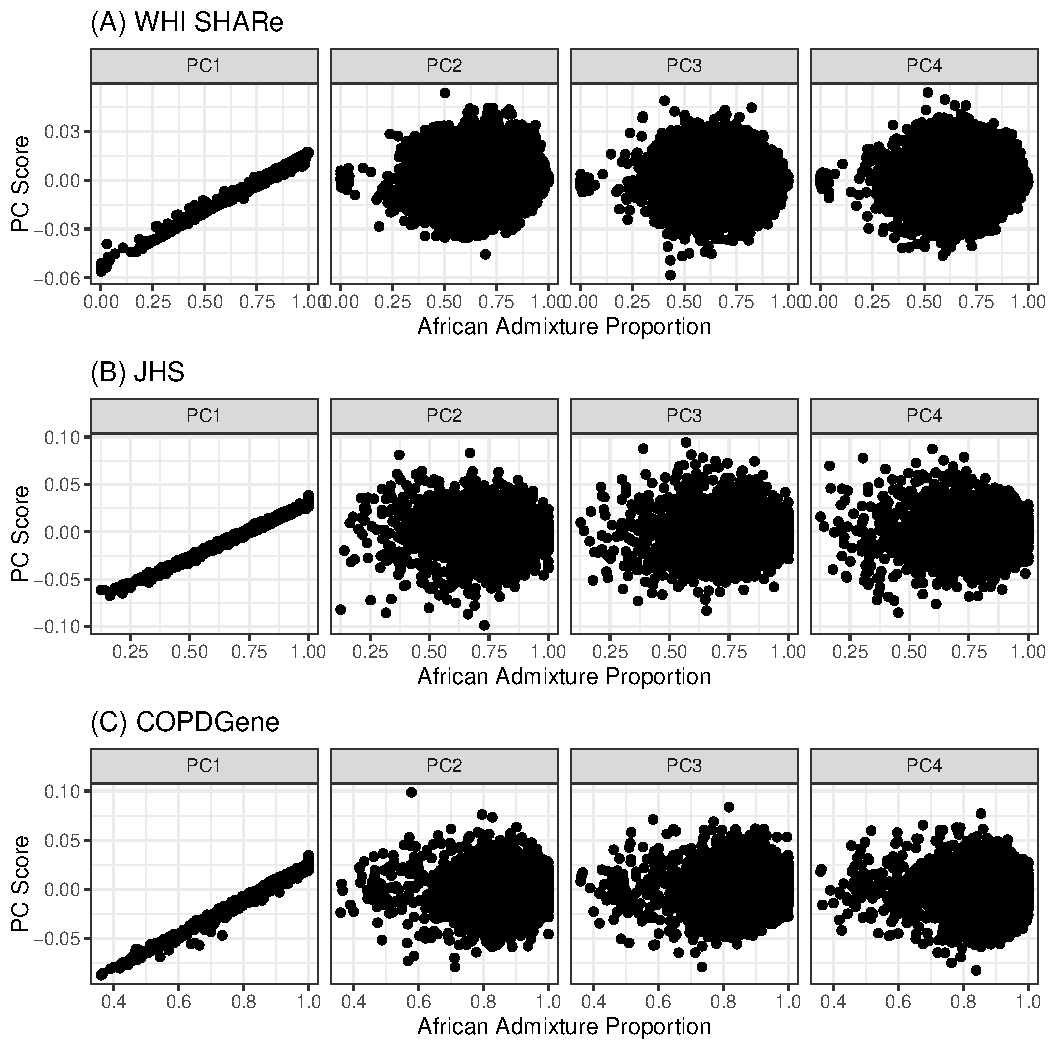
\includegraphics[width=\textwidth]{figs/pcs_vs_global/pcs_vs_global}
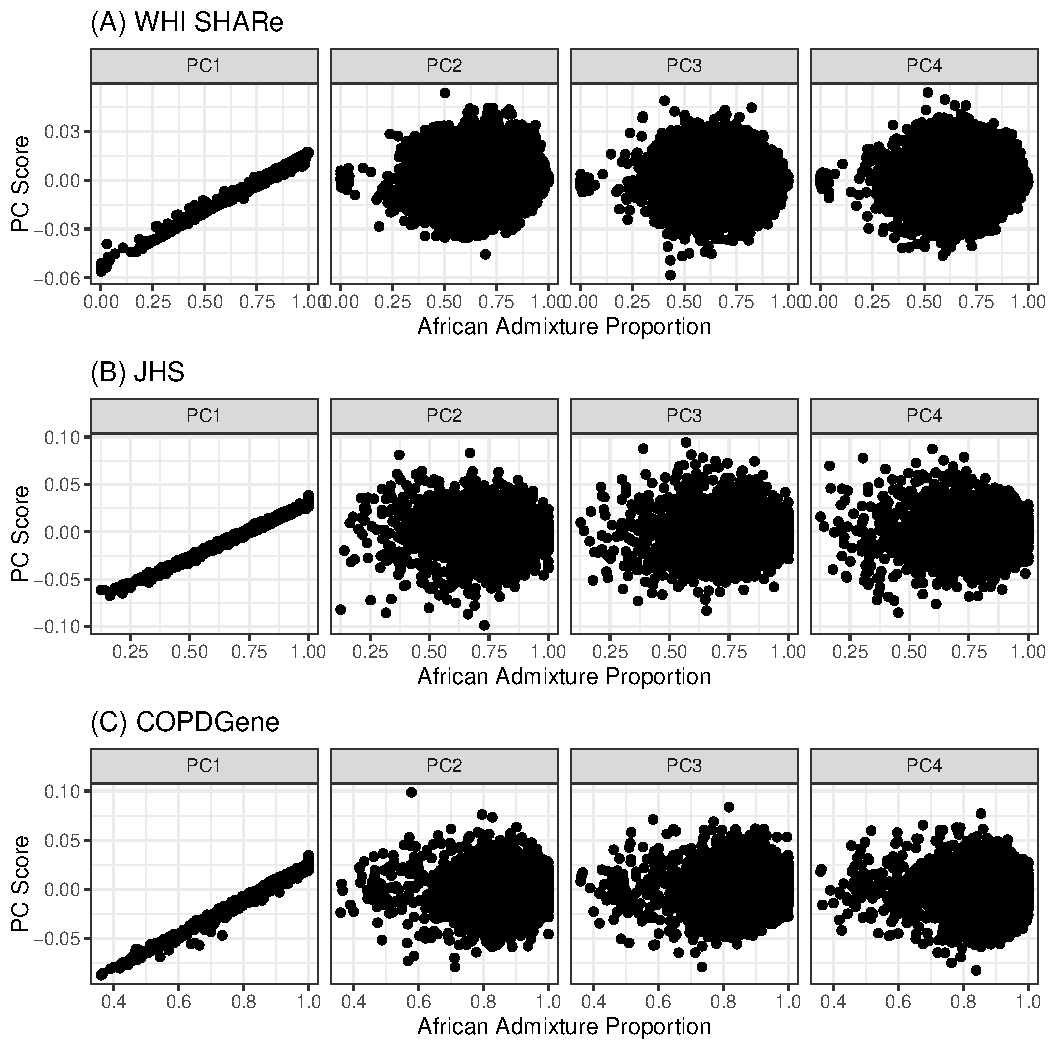
\includegraphics[width=\textwidth]{figs/finalfigs/figS1_pcs_vs_global}
\caption[Scatterplots of estimated admixture proportions versus the first four PCs, without LD-based filtering or pruning.]{Scatterplots of estimated African admixture proportions versus the first four PCs in (A) WHI SHARe, (B) TOPMed JHS, and (C) TOPMed COPDGene African Americans. Here we consider PCs that were generated on the entire set of SNPs (i.e., without any prior LD-based filtering or pruning).}
\label{fig:pcsvsglob}
\end{figure}

\begin{figure}
\center
%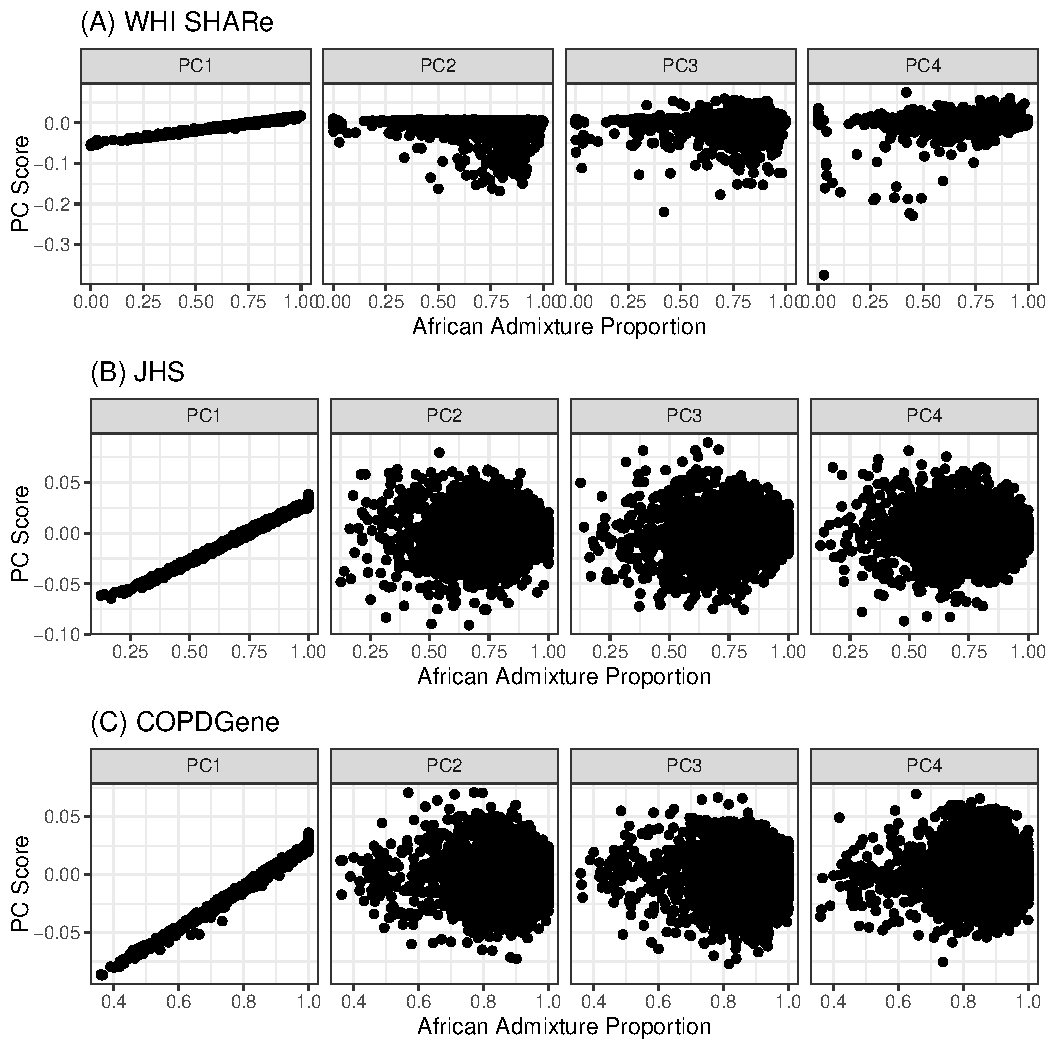
\includegraphics[width=0.9\textwidth]{figs/pcs_vs_global/pruned_pcs_vs_global}
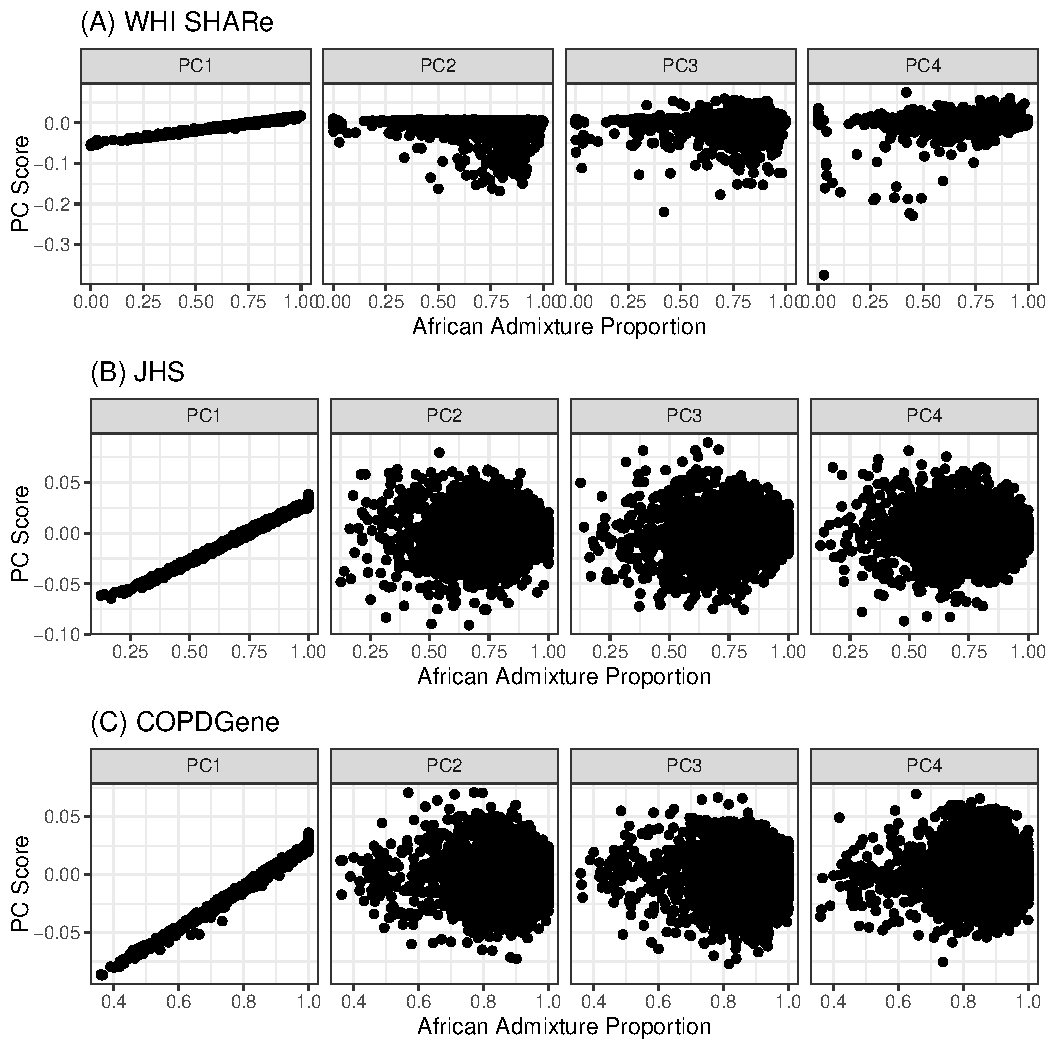
\includegraphics[width=0.9\textwidth]{figs/finalfigs/figS2_pruned_pcs_vs_global}
\caption[Scatterplots of estimated admixture proportions versus the first four PCs, with LD-based filtering and pruning.]{Scatterplots of estimated African admixture proportions versus the first four PCs in (A) WHI SHARe, (B) TOPMed JHS, and (C) TOPMed COPDGene African Americans. Here we consider PCs that were generated after both LD pruning ($r^2 = 0.1$, window size = 0.5 Mb) and filtering previously identified high-LD regions (Table \ref{tab:highLD}).}
\label{fig:prunedpcsvsglob}
\end{figure}




\section{Comparison of PCA Pre-Processing Choices}
\label{sec:comparefilters}

We have shown that adjusting for principal components that capture small regions of the genome rather than genome-wide ancestry can induce spurious associations in genome-wide association studies.
This problematic behavior occurred in our analysis of genotype data from WHI SHARe African Americans when PCs were generated using all 551,025 available SNPs or if we excluded regions identified in the literature as being potentially problematic for PCA (Table \ref{tab:highLD}).
However, problems were ameliorated when we used PCs that were generated after strict LD pruning, using an $r^2$ threshold of 0.1 and window size of 0.5 Mb.
In this section, we further investigate the behavior of PCs generated after different filtering techniques.

Many authors have suggested using an $r^2$ threshold of 0.2 for LD pruning prior to running PCA \citep{prive2018, weale2010, galinsky2016, zou2010, fellay2007, reed2015, novembre2008, anderson2010}.
Furthermore, this threshold is the default for LD pruning software such as \texttt{SNPRelate} \citep{snprelate}.
However, in our analysis of WHI SHARe data, we found that using an $r^2$ threshold of 0.2 prior to running PCA still led to one of the top PCs (the fourth) being highly correlated with small regions of the genome, while if we used a stricter threshold of 0.1 the peaks have disappeared (at least for the top four PCs).
See Figure \ref{fig:corr-compare-prune} for a comparison of the correlation between PCs and genotypes in WHI SHARe African Americans across different choices of $r^2$ threshold.

When performing LD pruning, another choice that practitioners have to make is the window size. 
In the literature, various window sizes have been suggested, including 10 Mb \citep{conomos2016}, 2 Mb \citep{weale2010}, or 0.5 Mb (the \texttt{SNPRelate} default), and others have suggested that window size may not have a big impact \citep{zou2010}.
Similar to the latter, in our analysis of WHI SHARe data we see little difference in the correlation between PCs and genotypes across different choices of window sizes: see Figure \ref{fig:corr-compare-window}.
Smaller window sizes are less computationally intensive, so we used the window size of 0.5 Mb for the remainder of our analyses.

Finally, we also considered filtering out regions that were highly correlated with PCs in our own data, as has been done previously \citep{novembre2008, prive2018}.
To implement this data-based filtering, we investigated the SNP loadings for each of the top four PCs. 
Starting with the second PC, we found the SNP on each chromosome with the largest loading: if this loading was larger than 0.005, we excluded the SNP and all SNPS within $M$ Mb; if the loading was small, we kept all SNPs on the chromosome.
(We considered $M = 1, 5, 10$, and $20$ Mb.) 
We repeated this process for PCs 3 and 4, then re-ran PCA using the remaining SNPs.
Using these new PCs, we re-calculated SNP loadings and looked to see if there were still regions of the genome that were driving the PCs.
If so, we repeated the entire process.
This data-based filtering process is very tedious, and even after four rounds of exclusions with $M = 5$ Mb we found that the problematic behavior did not totally go away (Figure \ref{fig:corr-compare-exclude}).

In WHI SHARe data, at least, strict LD pruning is the most effective of the pre-processing steps that we considered in eliminating the correlation between PCs and genotypes in small regions of the genome.

\begin{figure}
\center
%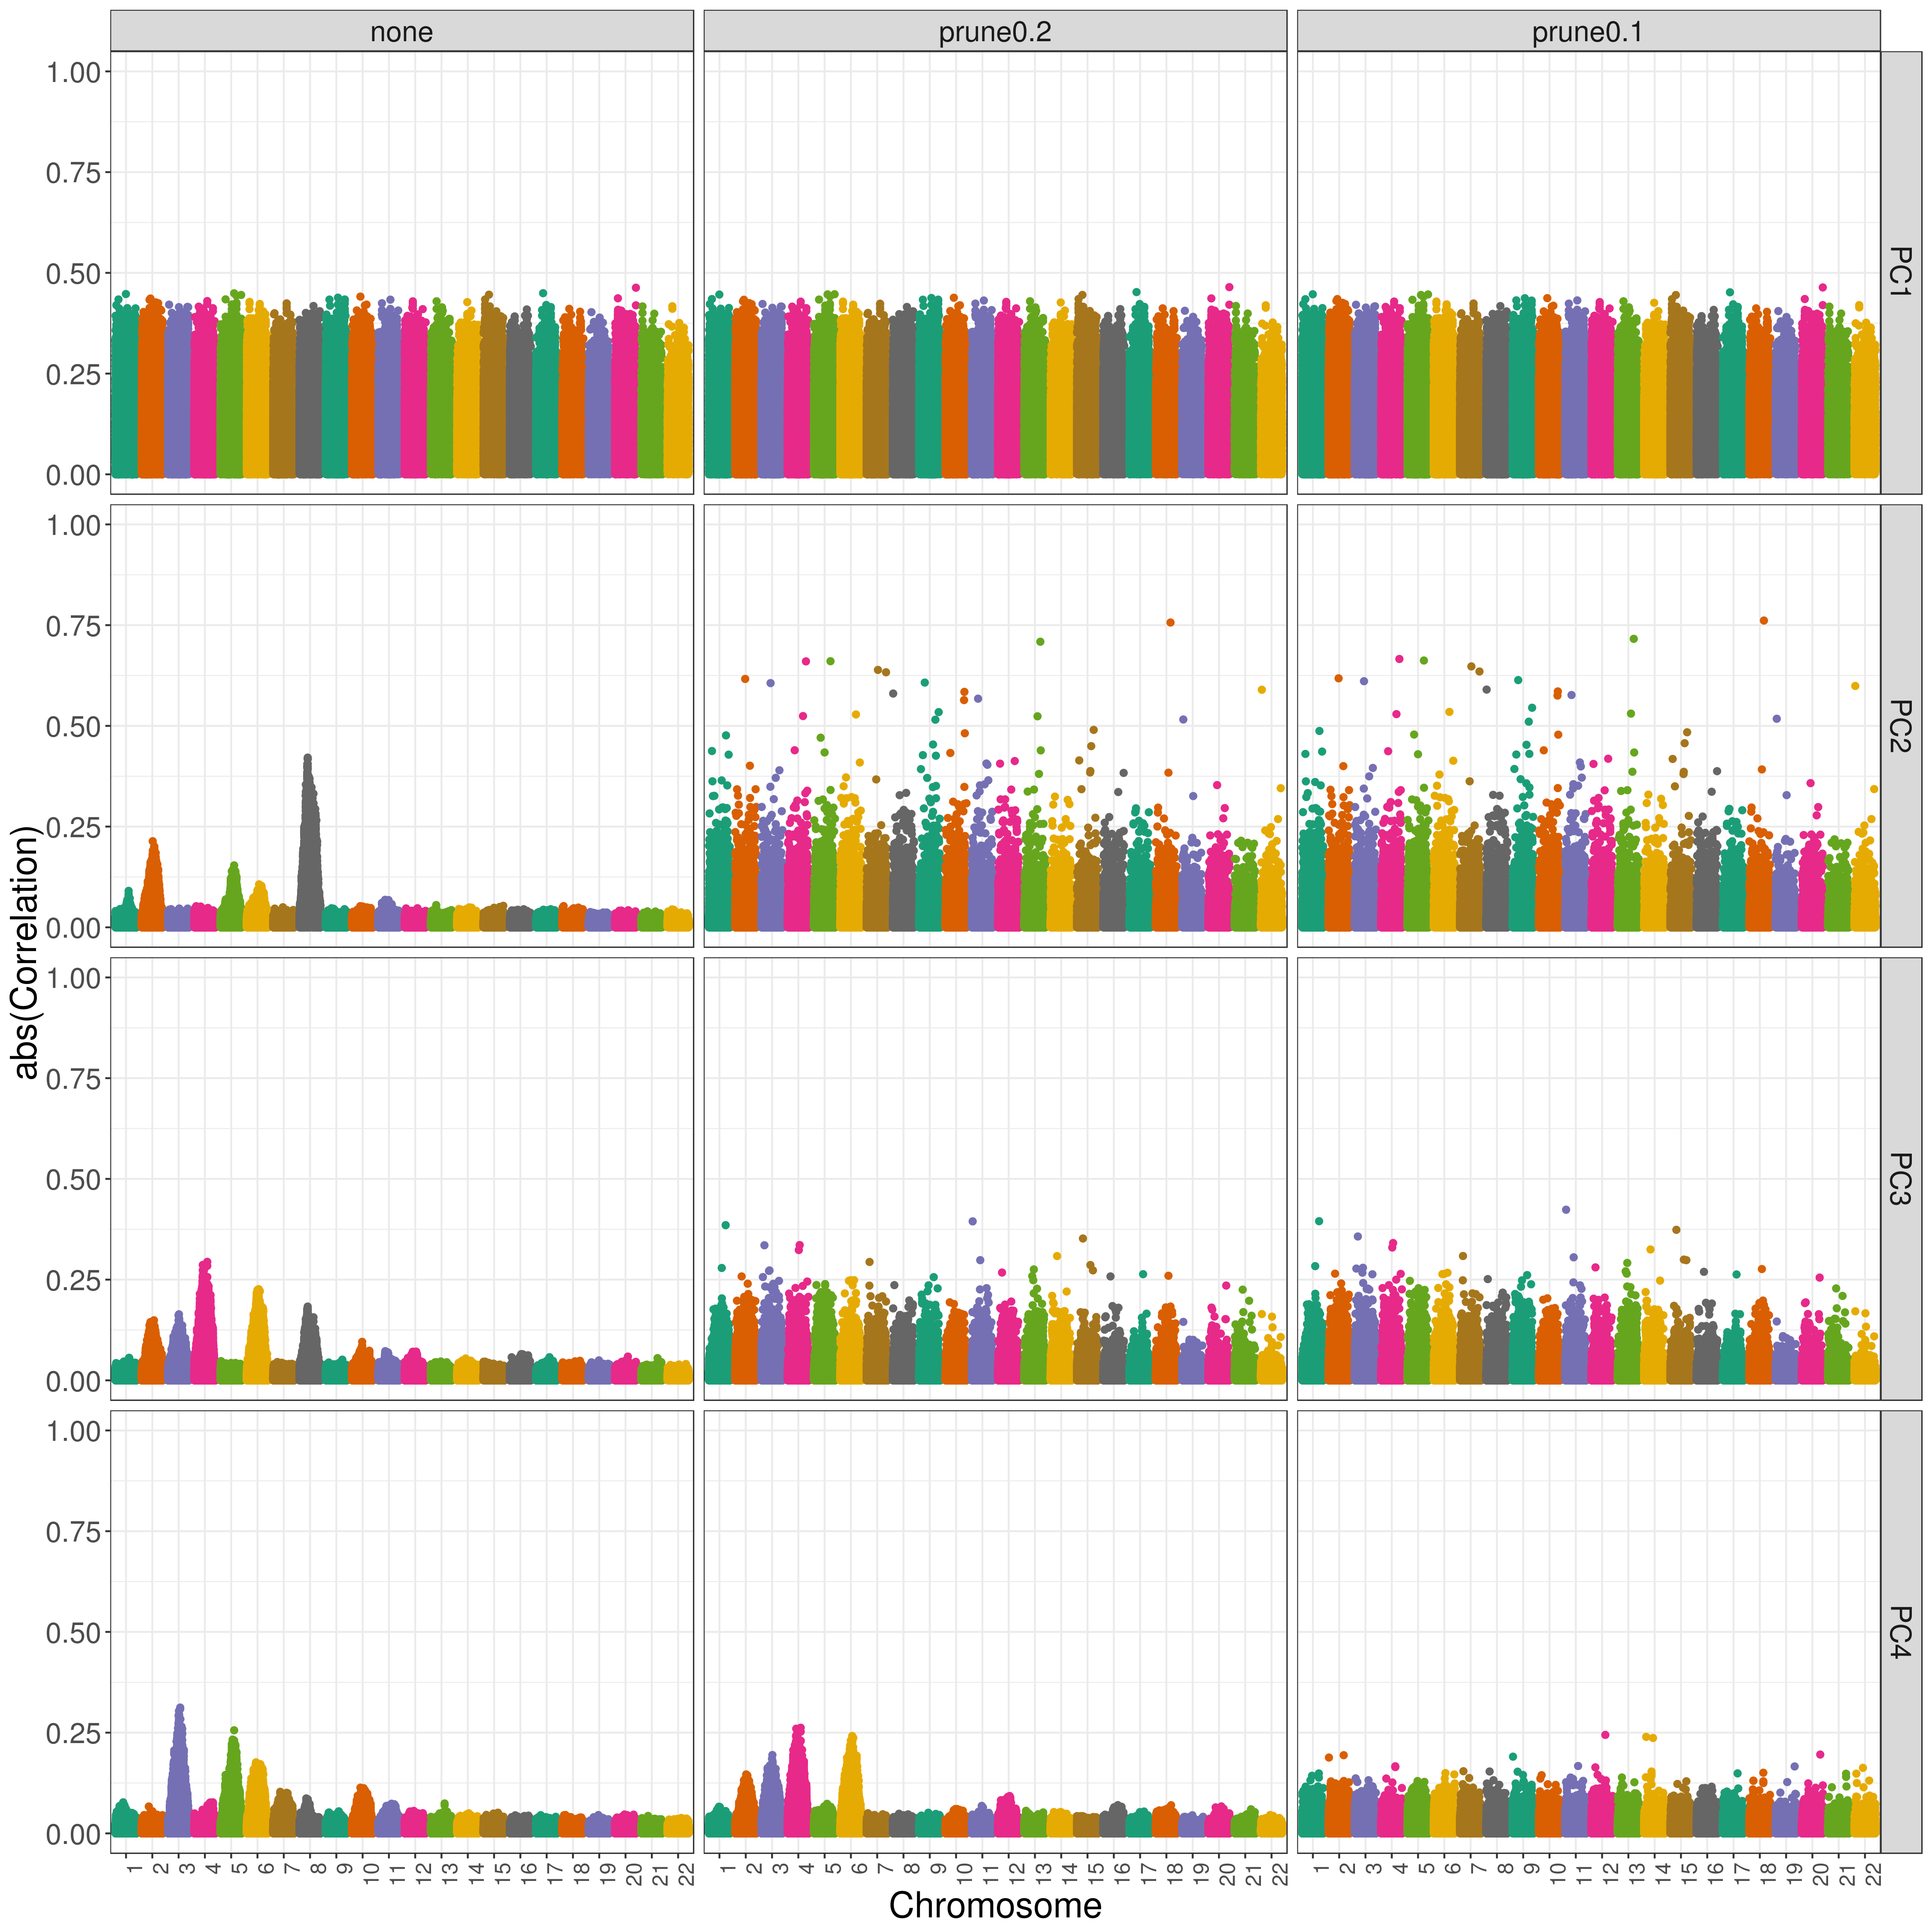
\includegraphics[width=\textwidth]{figs/pc_geno_corr/pc_geno_corr_compare_prune}
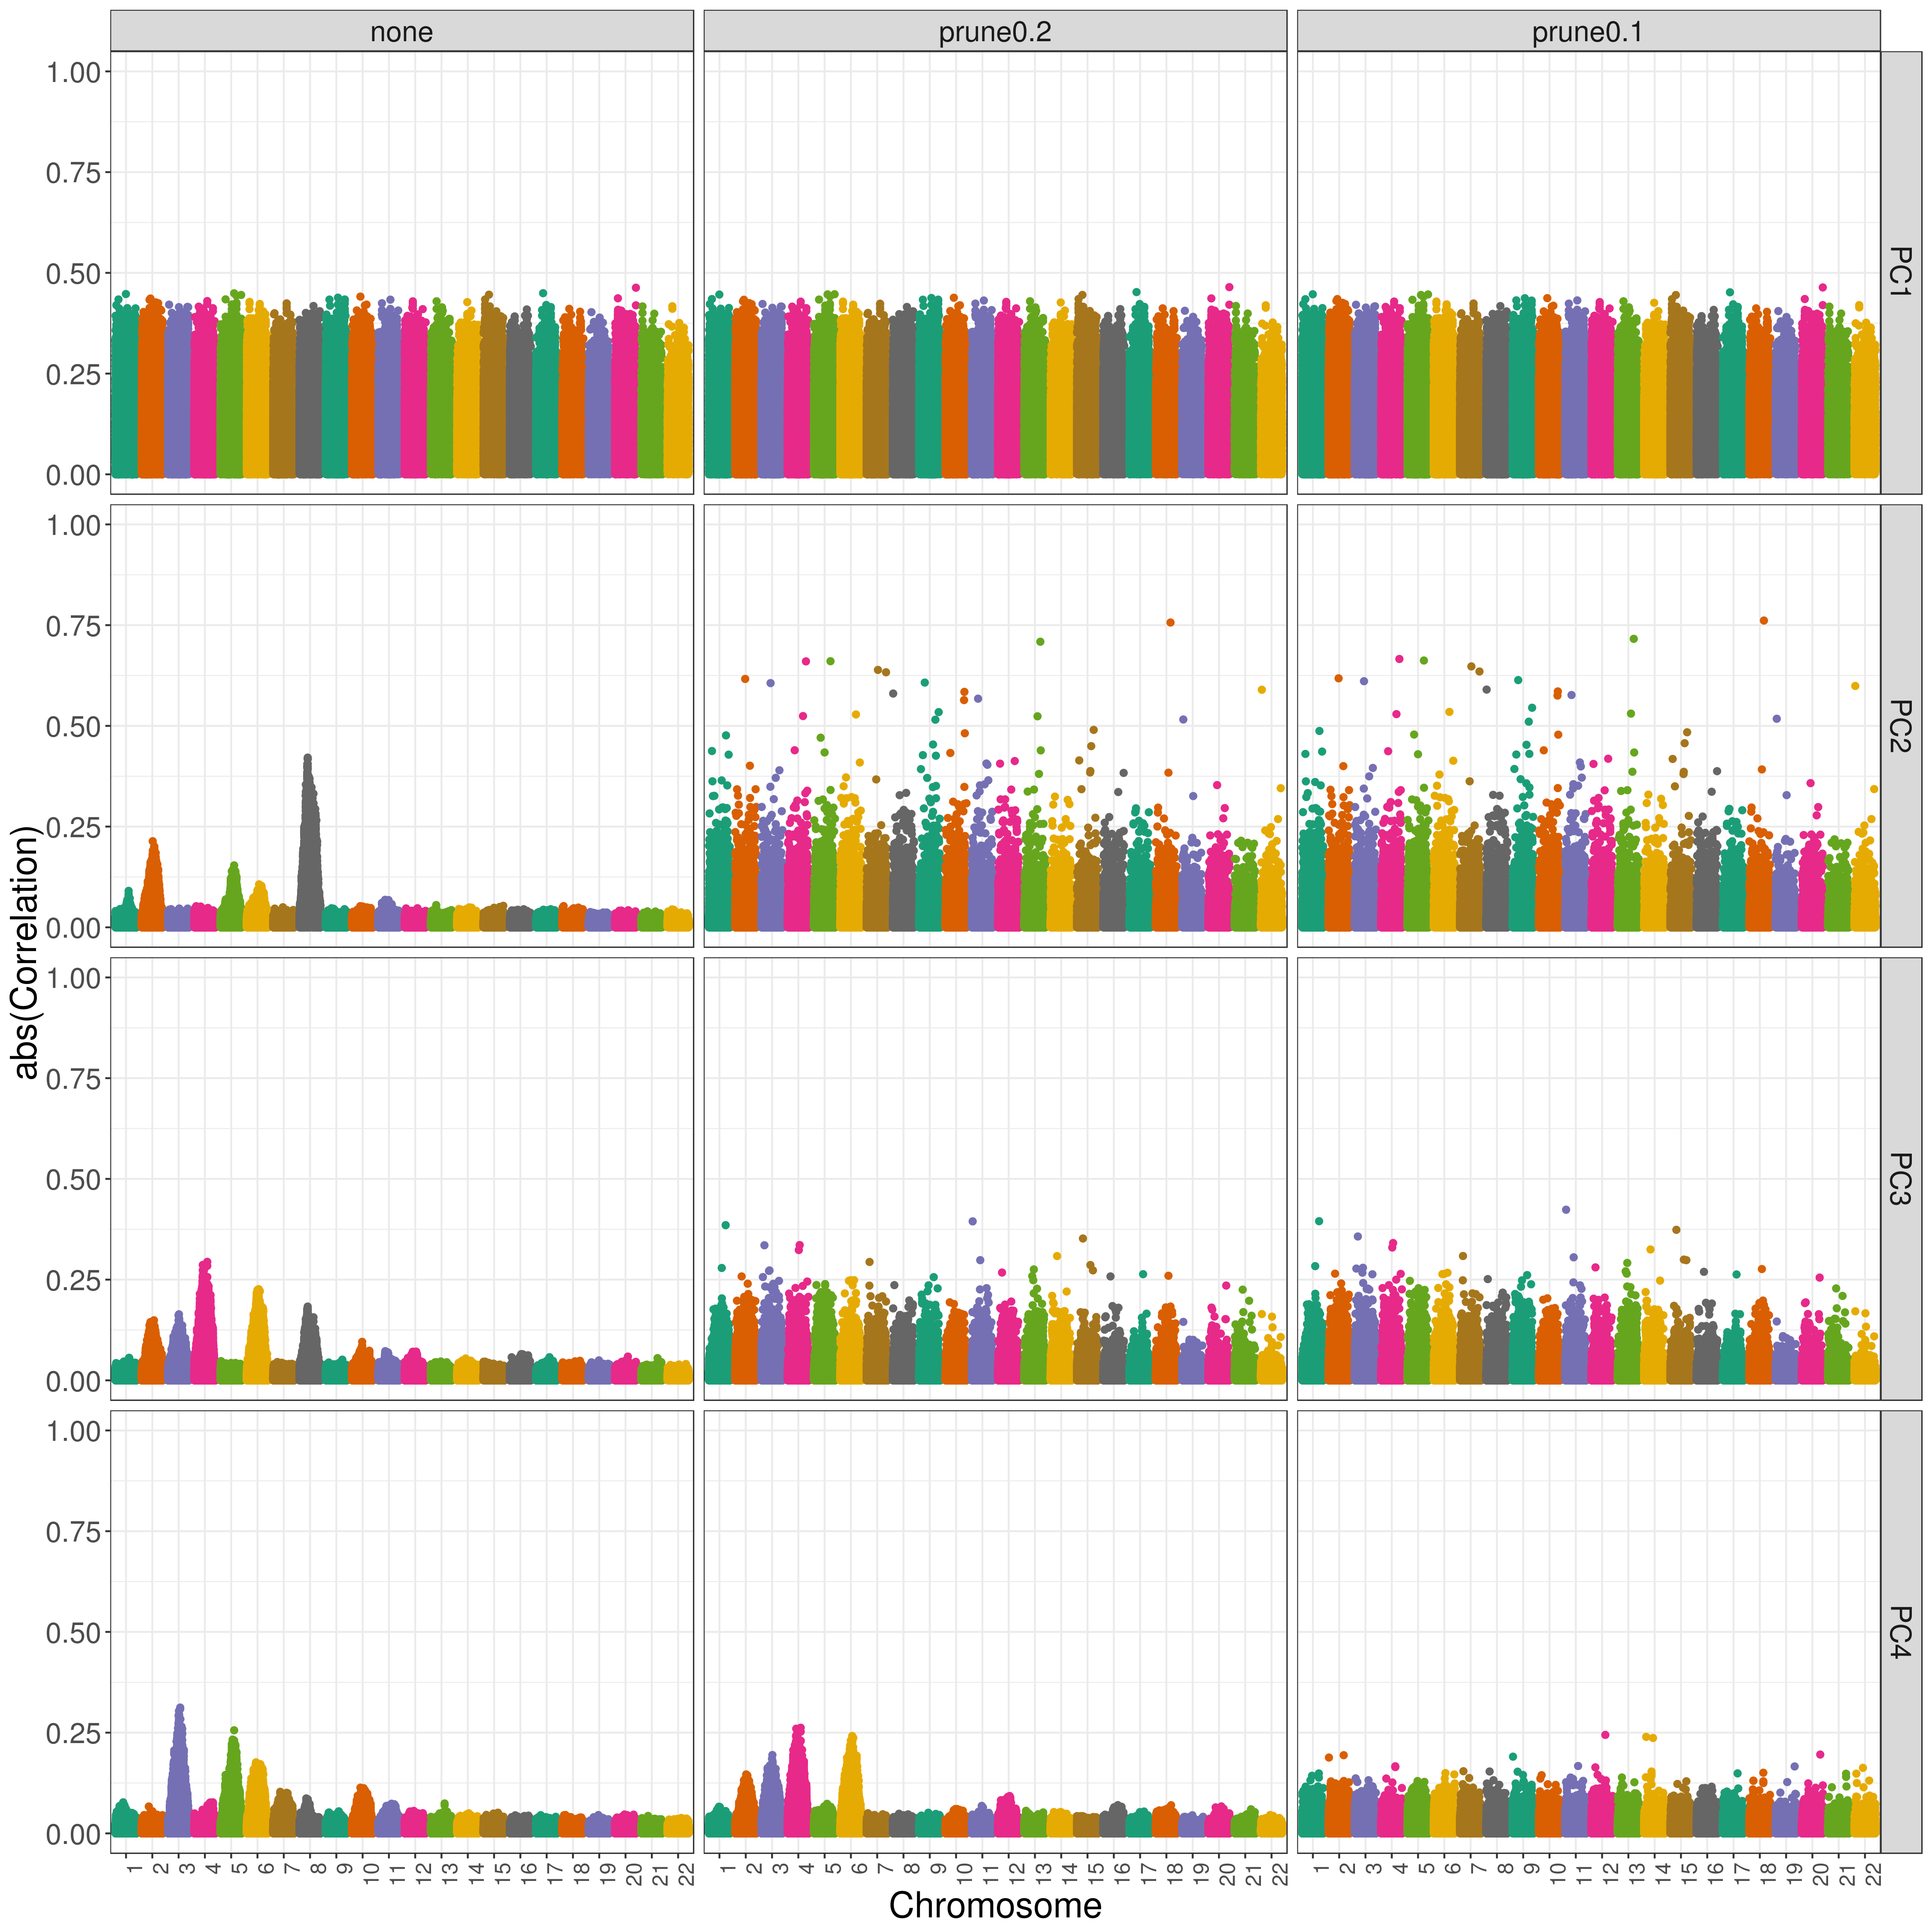
\includegraphics[width=\textwidth]{figs/finalfigs/figS3_pc_geno_corr_compare_prune}
\caption[Correlation between PCs and genotypes using different LD pruning thresholds.]{Correlation between PCs and genotypes in WHI SHARe African Americans using different LD pruning thresholds. Each panel plots the absolute value (abs) of the correlation between principal components and genotypes on the y-axis versus the position along the genome on the x-axis.  Panels are organized vertically according to which PC is being investigated (1, 2, 3, 4) and horizontally according to what $r^2$ threshold was used when running LD pruning prior to PCA (\textit{none}: no LD pruning, \textit{prune0.2}: LD pruning with an $r^2$ threshold of 0.2 and window size of 0.5 Mb, and \textit{prune0.1}: LD pruning with an $r^2$ threshold of 0.1 and window size of 0.5 Mb).}
\label{fig:corr-compare-prune}
\end{figure}

\begin{figure}
\center
%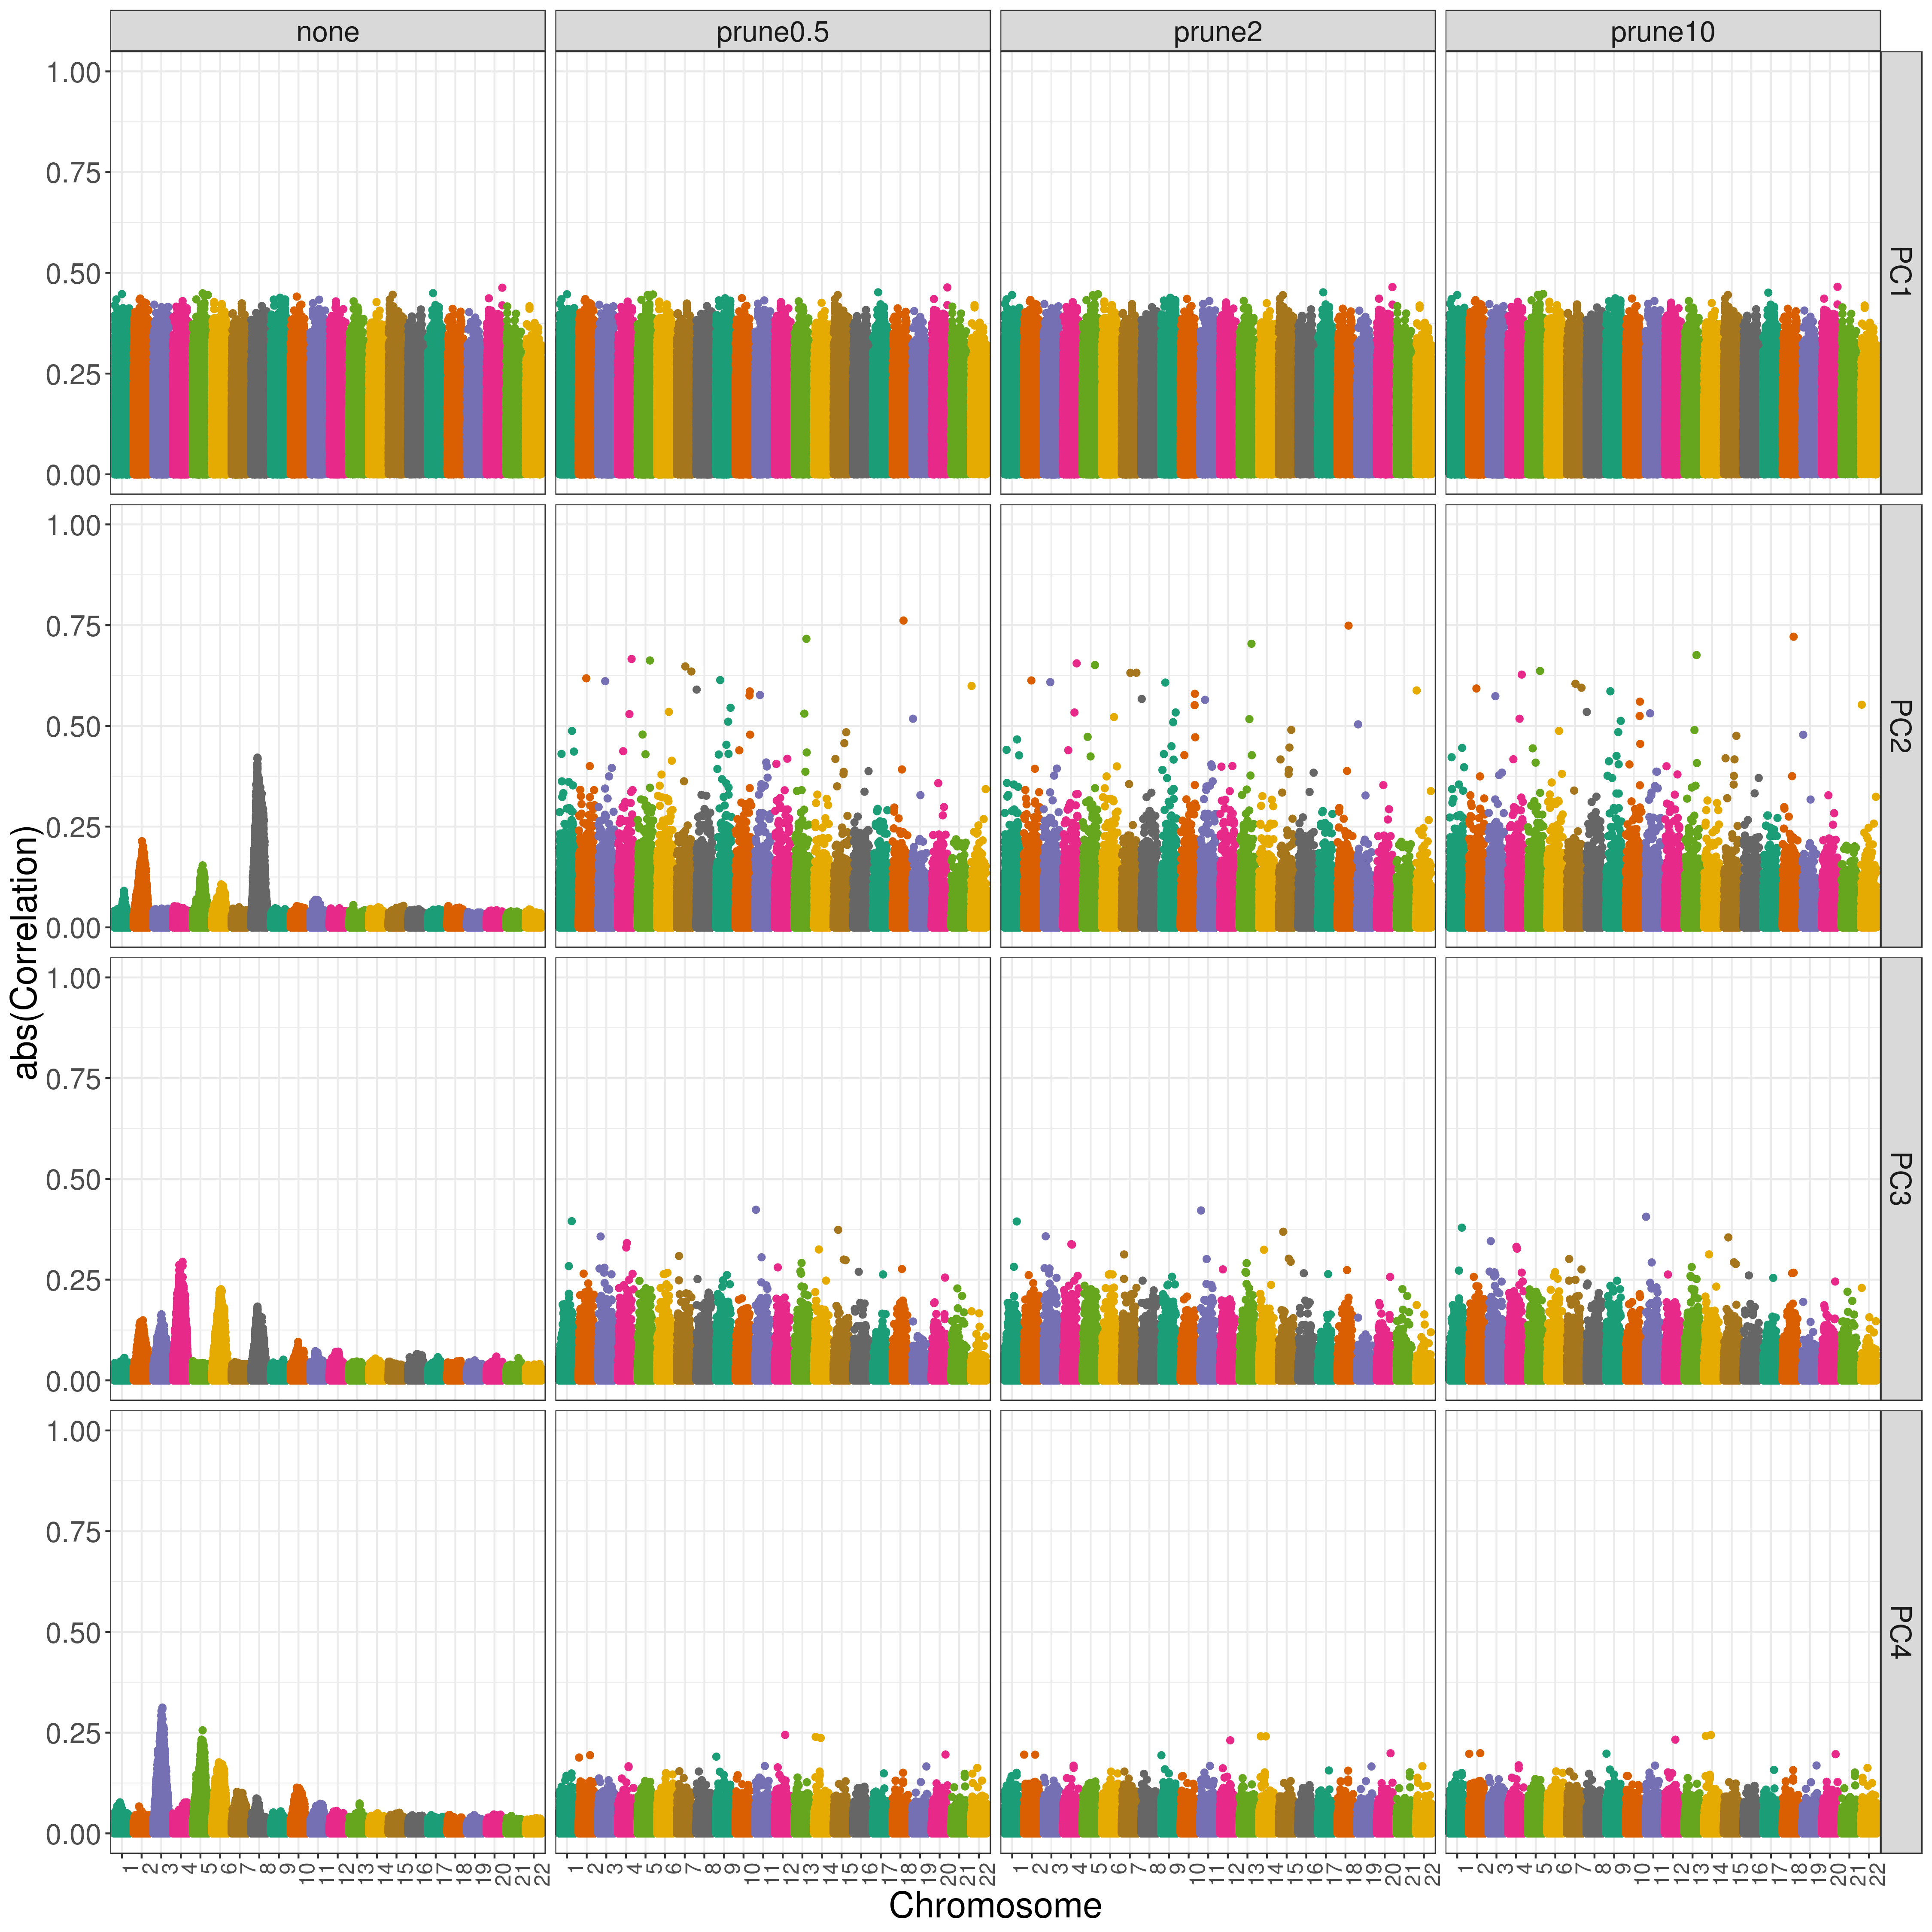
\includegraphics[width=\textwidth]{figs/pc_geno_corr/pc_geno_corr_compare_window}
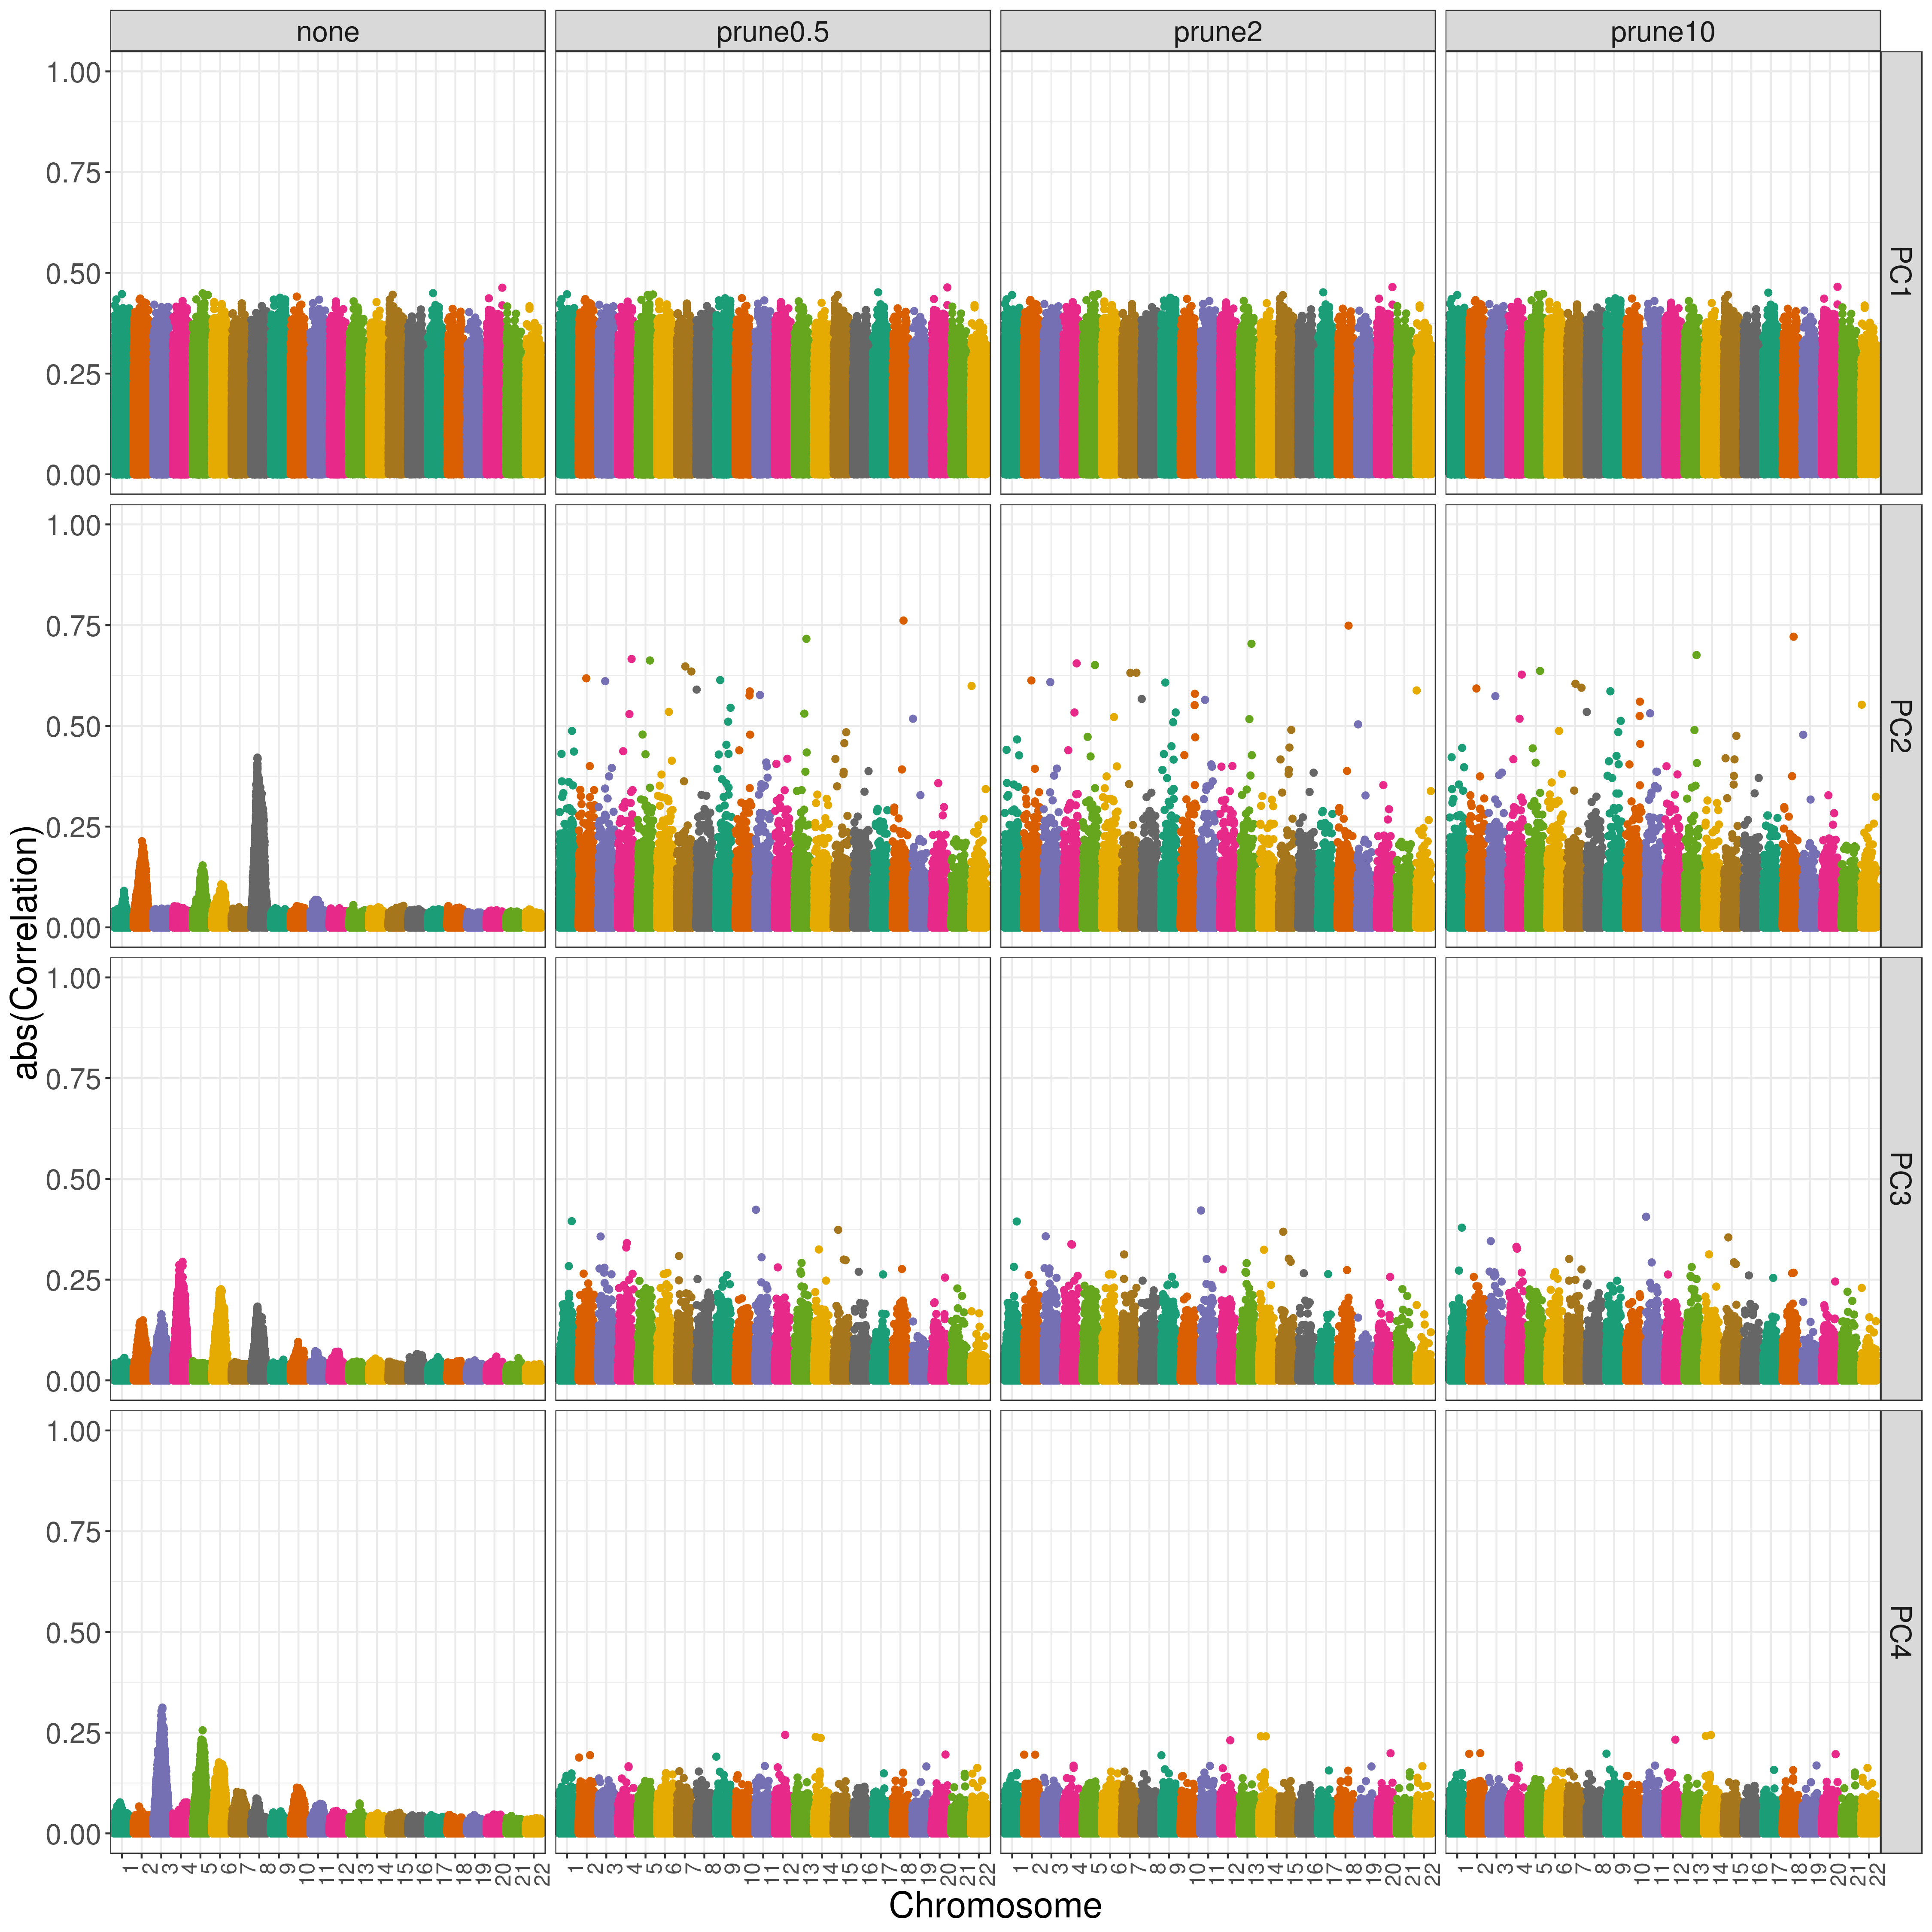
\includegraphics[width=\textwidth]{figs/finalfigs/figS4_pc_geno_corr_compare_window}
\caption[Correlation between PCs and genotypes using different LD pruning windows.]{Correlation between PCs and genotypes in WHI SHARe African Americans using different LD pruning window sizes. Each panel plots the absolute value (abs) of the correlation between principal components and genotypes on the y-axis versus the position along the genome on the x-axis.  Panels are organized vertically according to which PC is being investigated (1, 2, 3, 4) and horizontally according to what window size was used when running LD pruning prior to PCA (\textit{none}: no LD pruning, \textit{prune0.5}: LD pruning with an $r^2$ threshold of 0.1 and window size of 0.5 Mb, \textit{prune2}: LD pruning with an $r^2$ threshold of 0.1 and window size of 2 Mb, and \textit{prune10}: LD pruning with an $r^2$ threshold of 0.1 and window size of 10 Mb).}
\label{fig:corr-compare-window}
\end{figure}

\begin{figure}
\center
%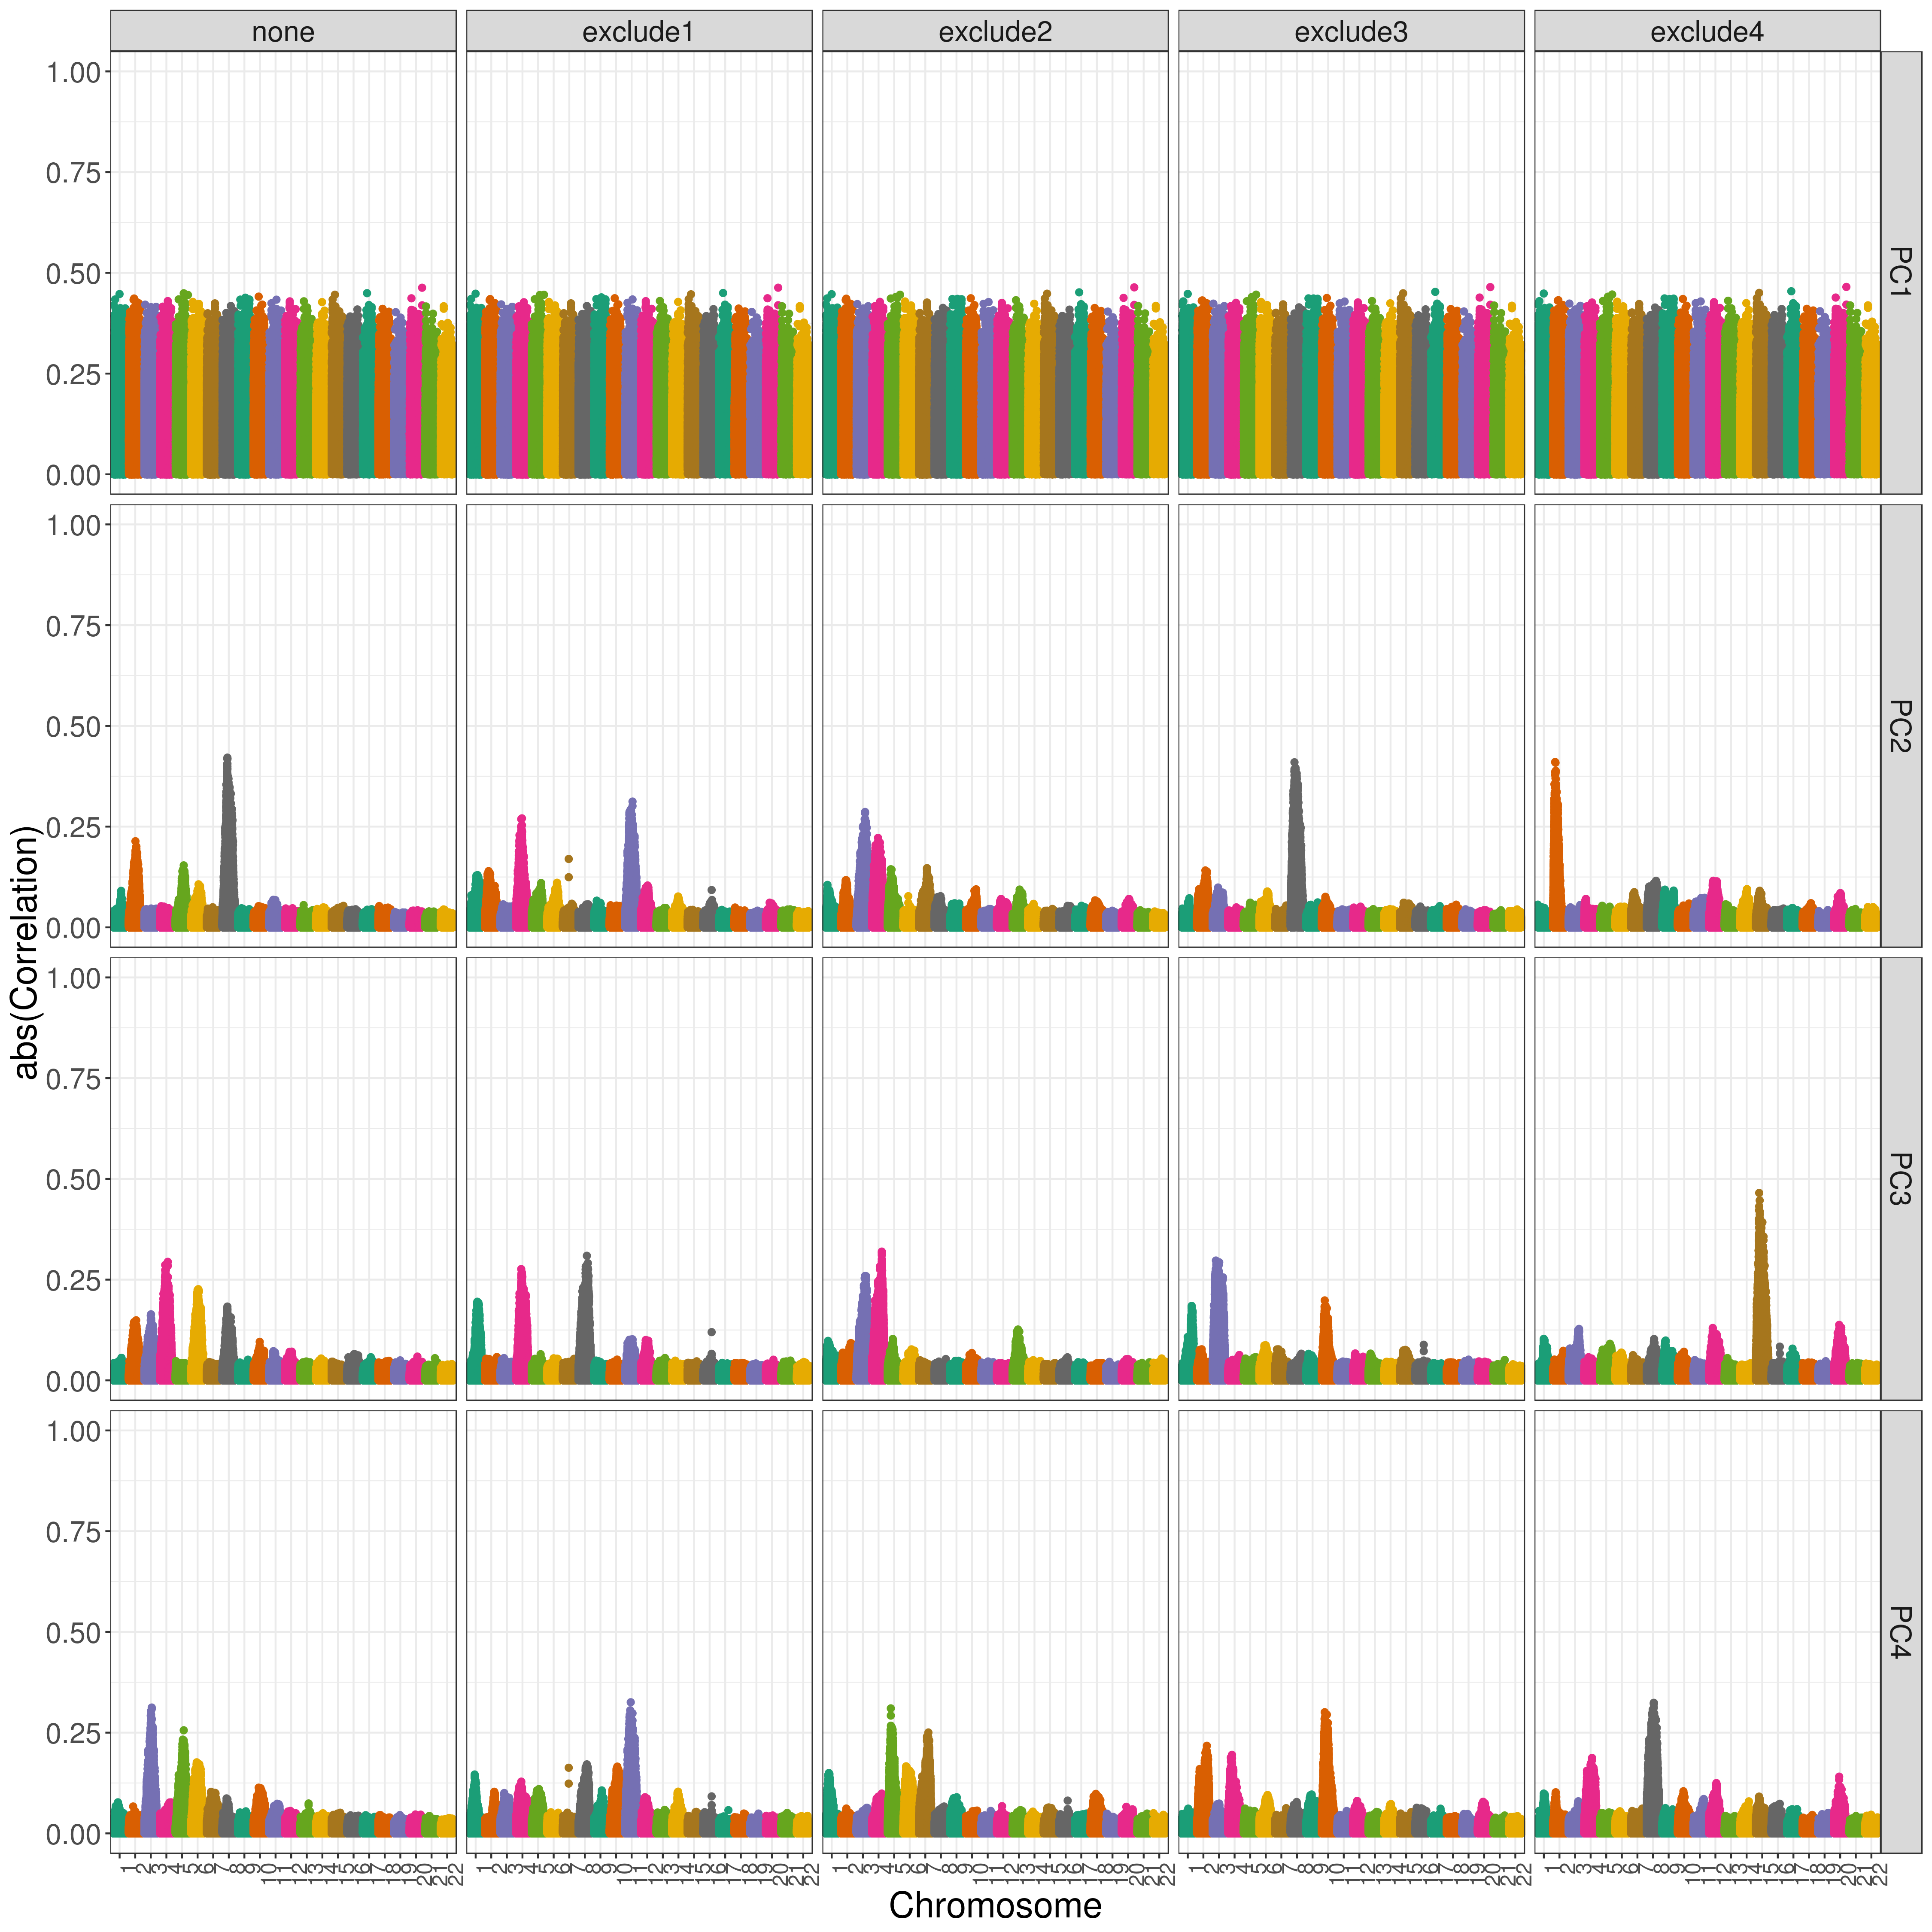
\includegraphics[width=\textwidth]{figs/pc_geno_corr/pc_geno_corr_compare_exclude}
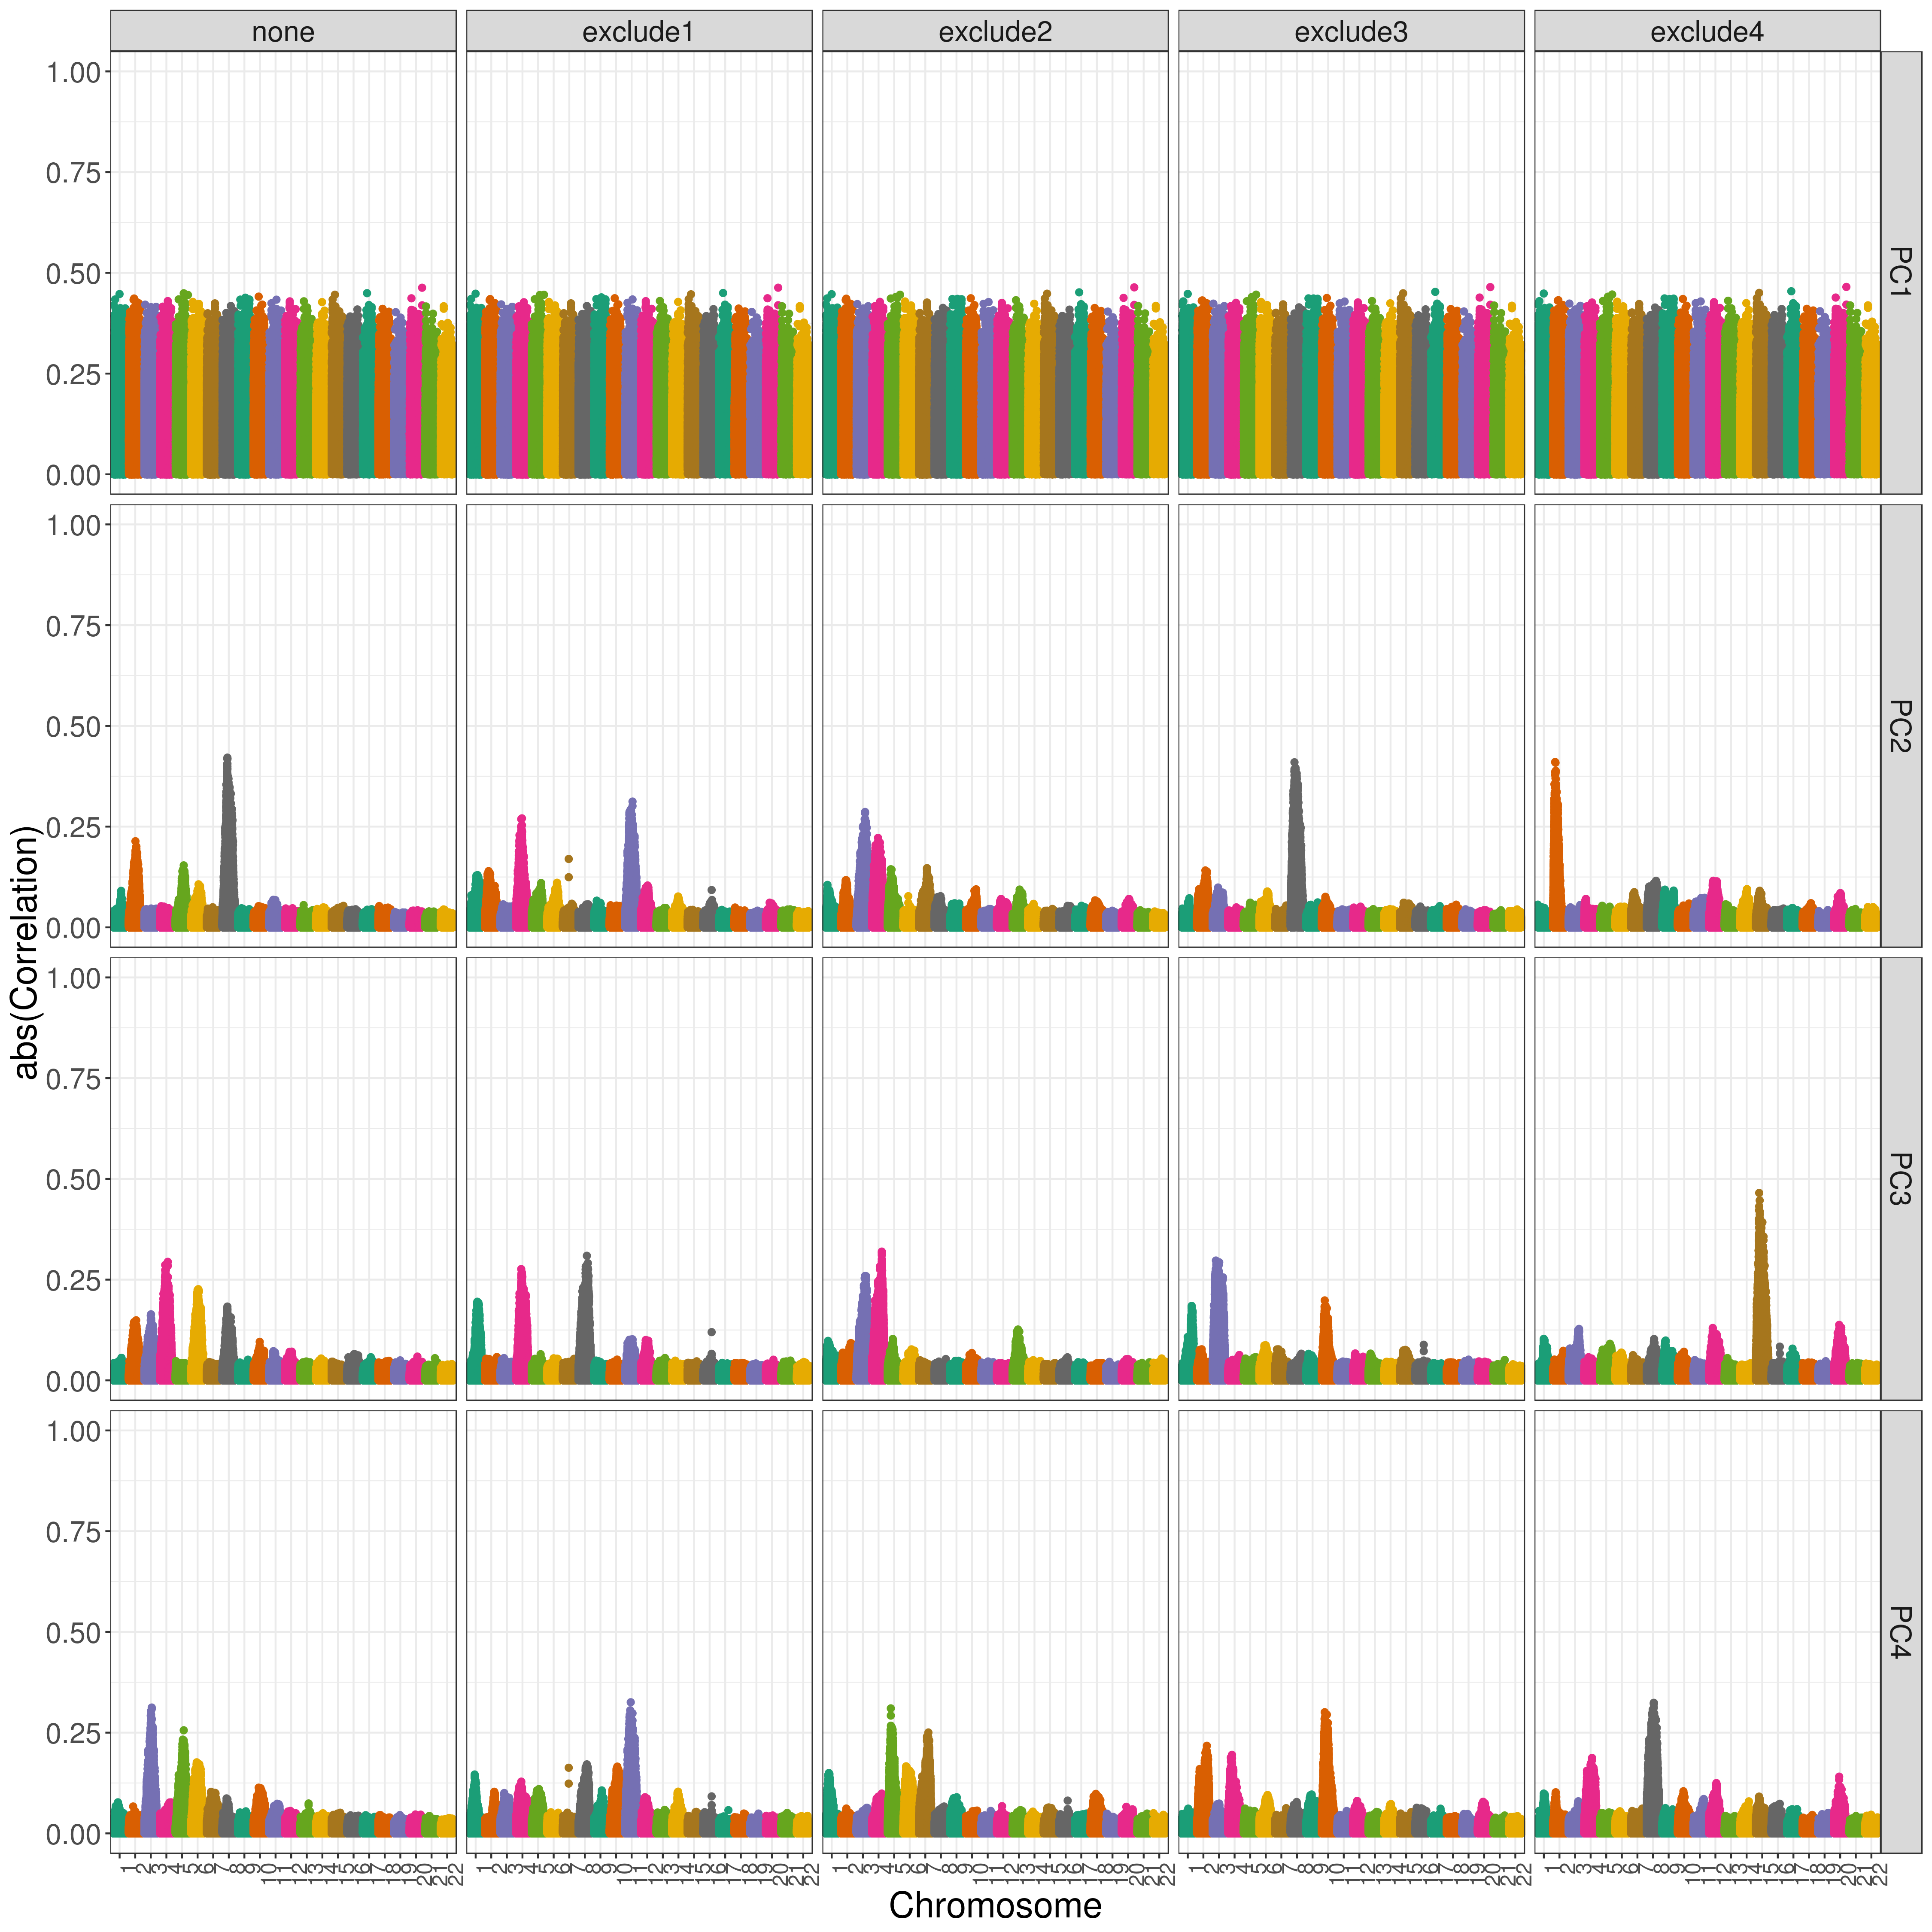
\includegraphics[width=\textwidth]{figs/finalfigs/figS5_pc_geno_corr_compare_exclude}
\caption[Correlation between PCs and genotypes using a data-based filtering process.]{Correlation between PCs and genotypes in WHI SHARe African Americans after multiple rounds of data-based exclusions. Each panel plots the absolute value (abs) of the correlation between principal components and genotypes on the y-axis versus the position along the genome on the x-axis.  Panels are organized vertically according to which PC is being investigated (1, 2, 3, 4) and horizontally according to the number of iterations of our procedure for excluding regions highly correlated with PCs in this sample (\textit{none}: no exclusions, \textit{exclude1}: one round of exclusions, \textit{exclude2}: two rounds of exclusions, etc.).}
\label{fig:corr-compare-exclude}
\end{figure}



\newpage
\section{Investigation of PCs in a European American Population}

We have shown that principal components can capture multiple local genomic features, rather than genome-wide ancestry, unless careful pre-processing is performed prior to running PCA.
This observation is not in itself novel, but note that the patterns we observe in WHI SHARe, JHS, and COPDGene African Americans do differ slightly from what has previously been observed in European populations.
In particular, in European populations a principal component might capture variation on a single chromosome \citep{zou2010, prive2020} whereas in these admixed populations we see PCs driven by contributions from variants across several chromosomes.
Although the focus of our work has been on admixed individuals, we were also able to run PCA on a sample of individuals with European ancestry using the COPDGene European Americans that we had excluded from our primary analyses. 
In this sample, we see patterns similar to those observed by previous authors, with the second and third principal components driven primarily by variants on a single chromosome: chromosome 11 (Figure \ref{fig:corr-Eur}).
This difference in what is captured by principal components in European populations versus admixed populations (i.e., variants on one chromosome versus multiple) has important implications: only when a PC captures \textit{multiple} local genomic features does the possibility of collider bias arise.
Thus, particular care must be taken when performing genome-wide association studies in admixed populations to ensure that models to do not adjust for principal components that are highly correlated with variants on distinct chromosomes.

\begin{figure}
\center
%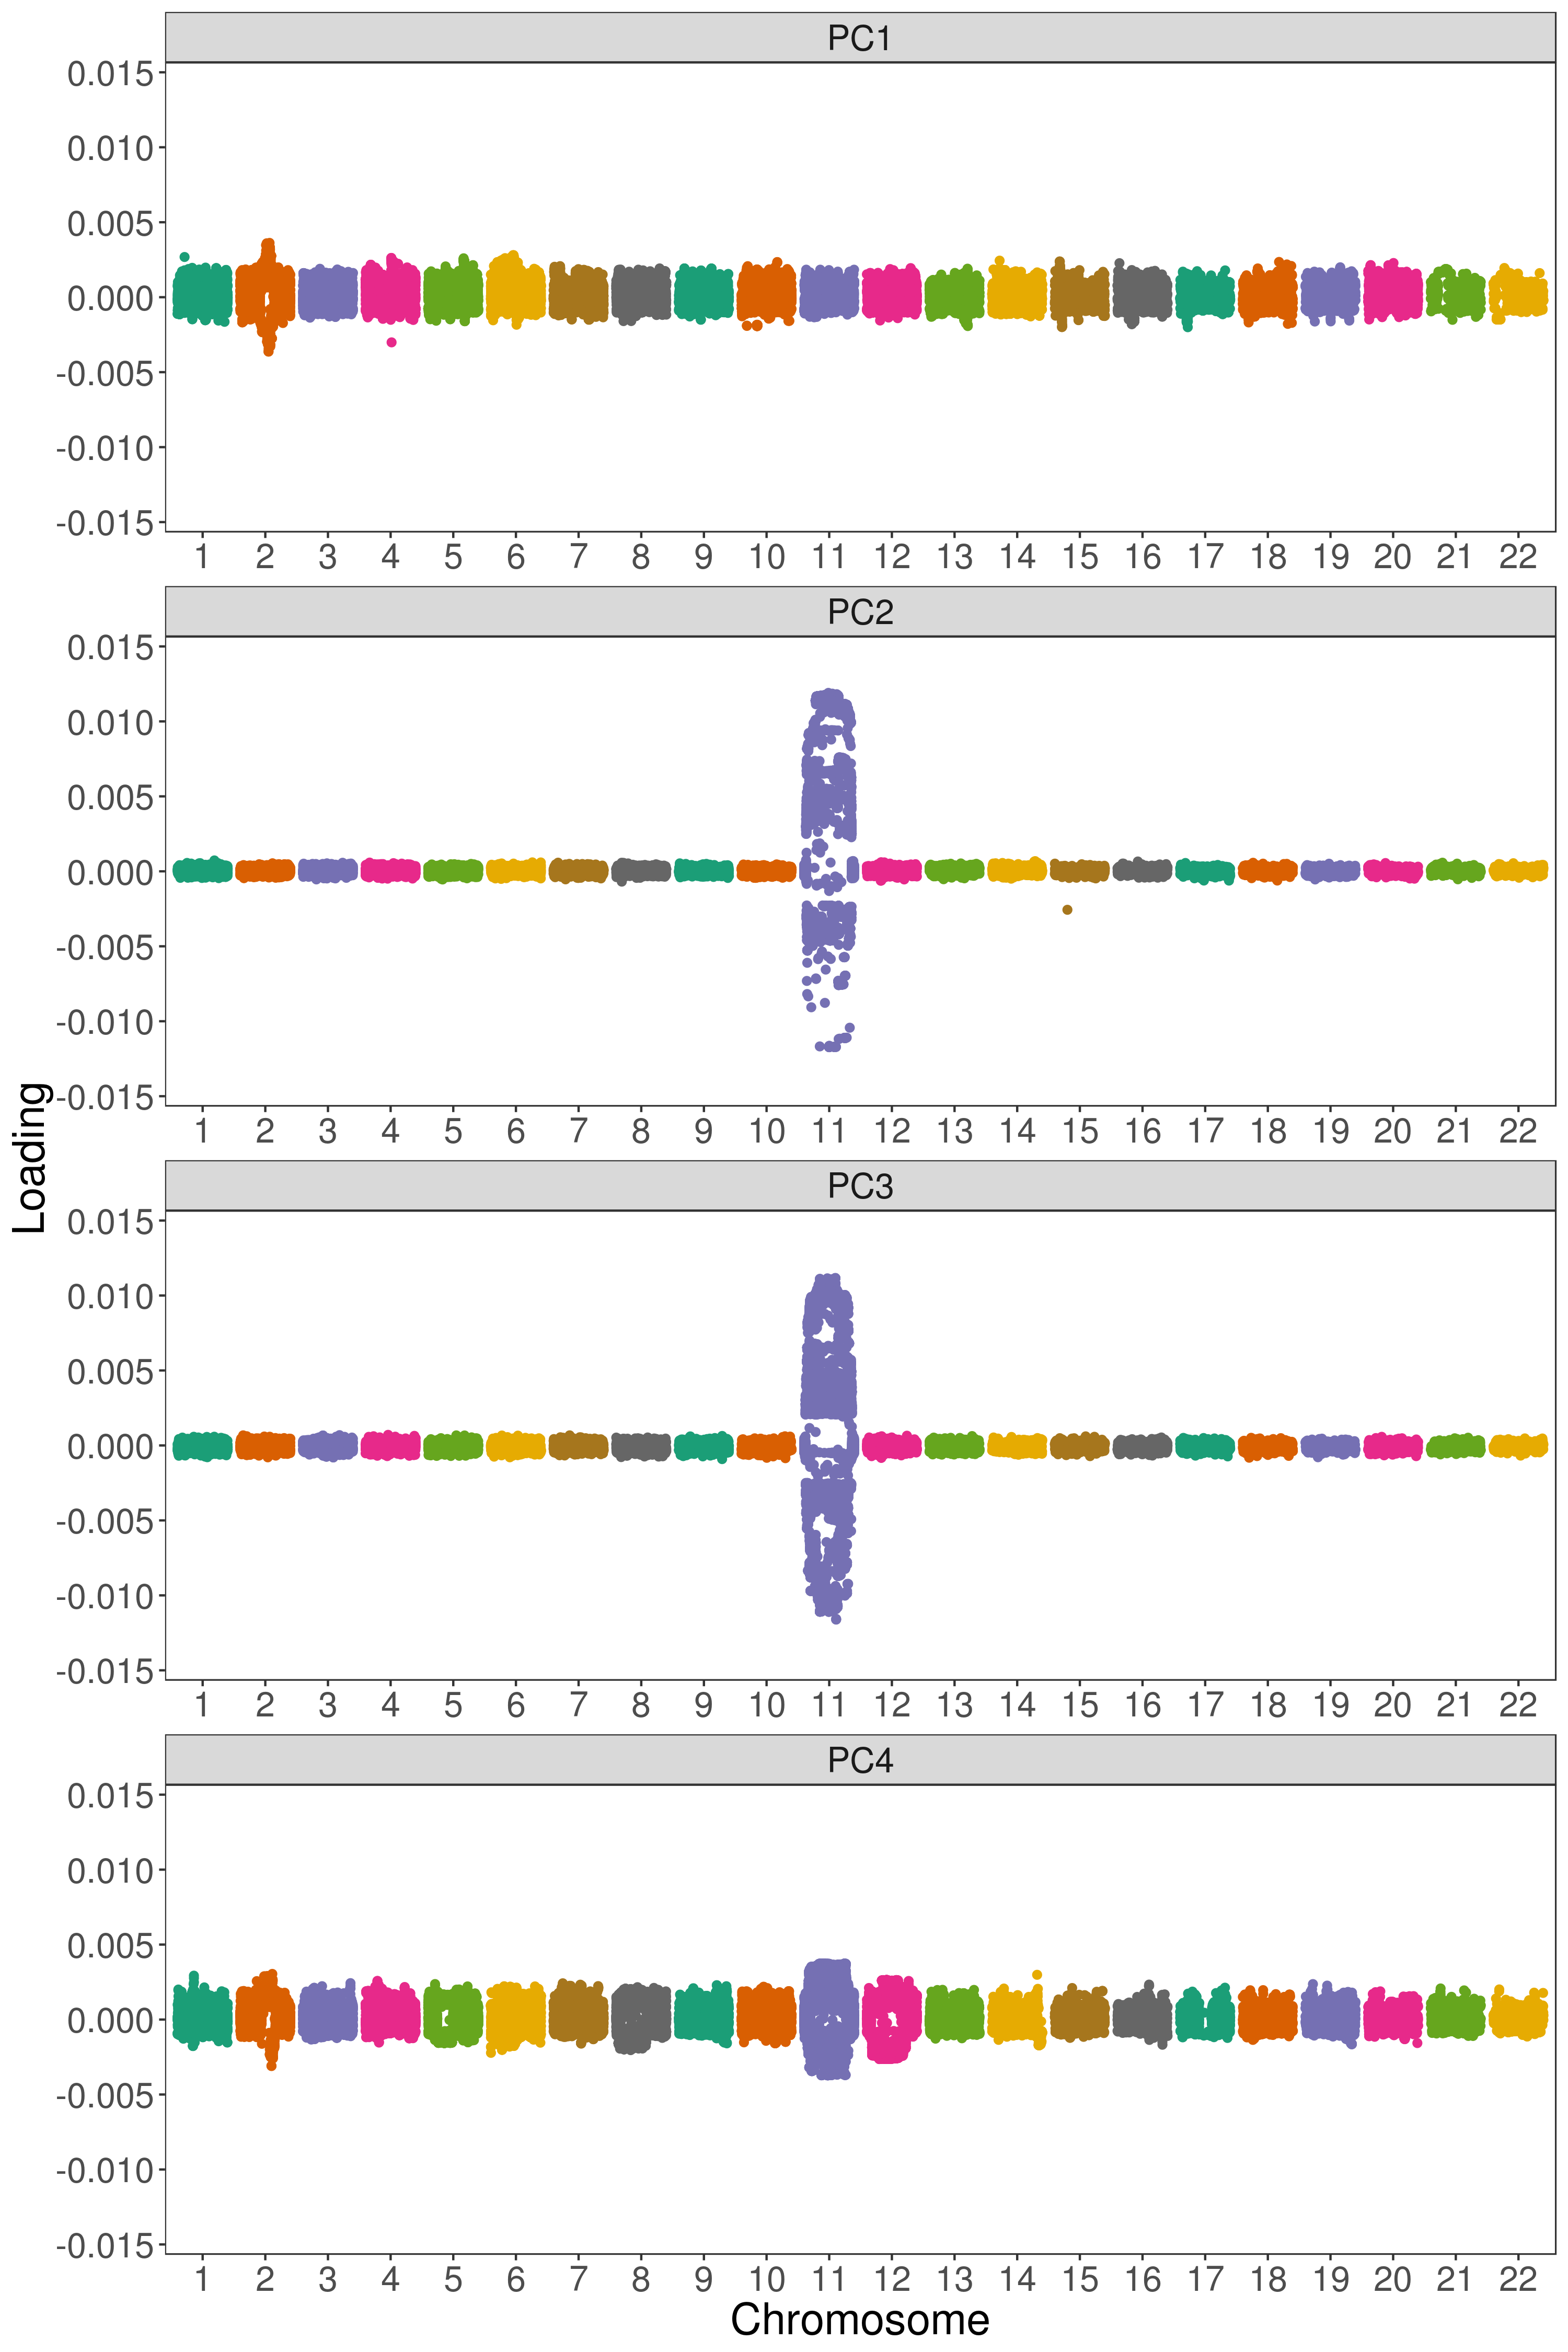
\includegraphics[width=0.8\textwidth]{figs/COPD/EUR_prune_FALSE_1_0_0.01_snprelate_load_1}
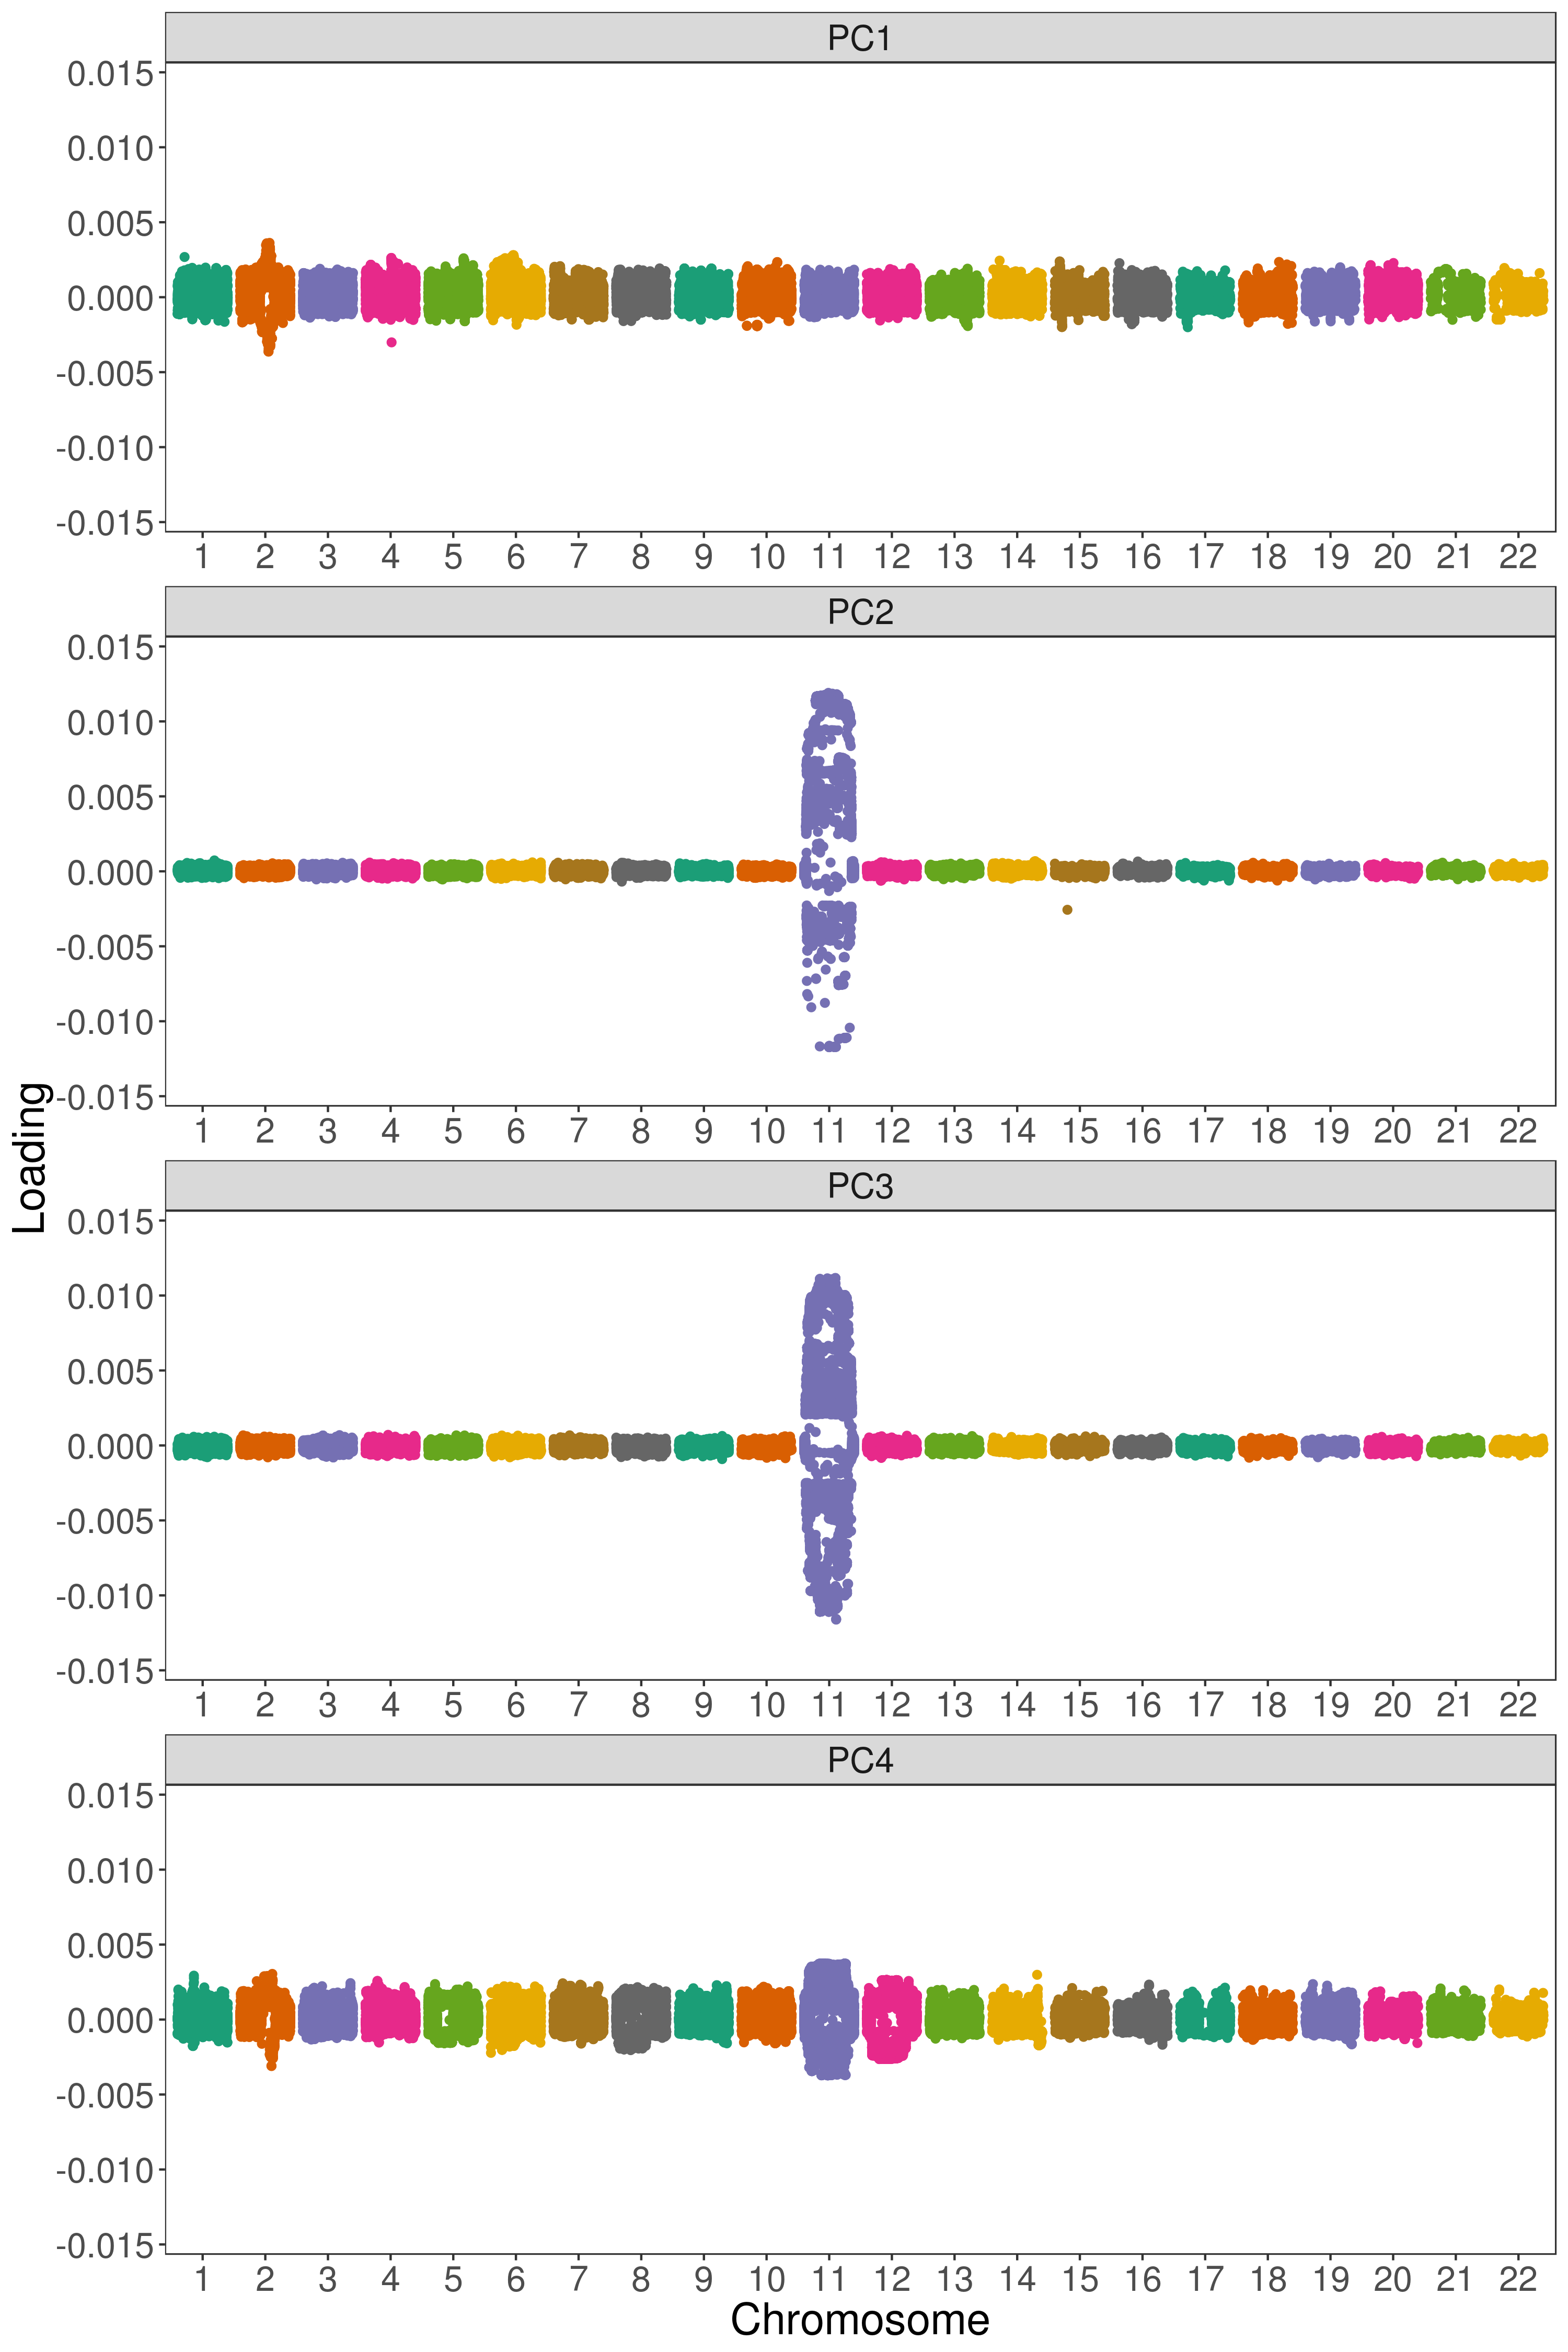
\includegraphics[width=0.8\textwidth]{figs/finalfigs/figS6_EUR_prune_FALSE_1_0_0.01_snprelate_load_1}
\caption[SNP loadings in COPDGene European Americans.]{SNP loadings for naively generated PCs in COPDGene European Americans. Each panel plots the principal component loading (y-axis) versus the position along the genome (x-axis) for each variant. Panels are organized vertically according to which PC is being investigated (1, 2, 3, 4). Unlike in admixed populations, we see a single peak on chromosome 11.}
\label{fig:corr-Eur}
\end{figure}


\newpage
\section{Derivation of Theoretical Results}
\label{sec:theory}

In the main paper, we present the expected effect size estimates for GWAS models using different techniques for adjusting for ancestral heterogeneity: see Equations (\ref{eqn:pi}), (\ref{eqn:unadjusted}), and (\ref{eqn:collider}).
Here, we provide details and simulation studies validating these theoretical results.

\subsection{Assumed data-generating mechanism}
\label{sec:datagen}

We consider an admixed population with two ancestral populations, $n$ individuals, and admixture proportions $\boldsymbol{\pi}_i = \begin{pmatrix} \pi_{i} & 1-\pi_{i} \end{pmatrix}^\top$ that are allowed to vary across the population. 
We refer to the two ancestral populations as \textit{Ancestral Population 1} and \textit{Ancestral Population 2}, with $\pi_i$ representing the genome-wide proportion of genetic material inherited by individual $i$ from Ancestral Population 1 and $1-\pi_i$ representing the proportion of genetic material inherited from Ancestral Population 2. 
We denote local ancestry by $\mathbf{a}_{ij} = \begin{pmatrix} a_{ij} & 2 - a_{ij} \end{pmatrix}^\top,$ where $a_{ij}$ and $2-a_{ij}$ are the number of alleles inherited by individual $i$ from Ancestral Populations 1 and 2, respectively, at position $j$.
Genotypes, quantified as the number of copies of some pre-specified allele carried by individual $i$ at position $j$, are represented by $g_{ij}$.
We consider two \textit{unlinked} variants $j = 1, 2$ (e.g., variants on distinct chromosomes) and assume that data are generated according to the following hierarchical model: 
\begin{align*}
\pi_i &\overset{\text{i.i.d.}}{\sim} F \text{ for some distribution } F\\
a_{ij} \mid \pi_i &\overset{\text{i.i.d}}{\sim} \text{Binomial}(2, \pi_i), \ j = 1, 2\\
g_{ij} \mid a_{ij}, \mathbf{p}_j &\overset{\text{ind.}}{\sim} \text{Binomial}(a_{ij}, p_{j1}) + \text{Binomial}(2-a_{ij}, p_{j2}), \ j = 1, 2 
\end{align*}
where $p_{j1}, p_{j2}$ are allele frequencies at position $j$ in Ancestral Populations 1 and 2, respectively. 
Since the two variants under consideration are unlinked, we assume that local ancestry and genotypes at these positions are conditionally independent.

We assume that our quantitative trait of interest $\mathbf{y}$ depends only on the genotype at position 1 ($j = 1$), and we allow for the possibility that the admixture proportions $\boldsymbol\pi$ have a direct effect on the trait (e.g., through environmental differences across ancestral populations). More specifically, we assume that this trait is generated according to $$y_i  = \beta_0 + \beta_1 g_{i1} + \beta_\pi \pi_i + \epsilon_i, \ \ \epsilon_i \overset{\text{i.i.d}}{\sim} (0, \sigma_\epsilon^2).$$
We refer to $\beta_1$ and $\beta_2$ as the true \textit{effect sizes} of variants 1 and 2, respectively. Since the trait only depends on the genotype at position 1, the true effect size of position 2 is $\beta_2 = 0$.
%We are interested in using genome-wide association studies (GWAS) and admixture mapping studies to investigate the association between loci 1 and 2 and the trait of interest. 

Assuming that data are generated according to the above-described mechanisms, and defining $E_\pi := E(\pi)$ and $V_\pi :=   \text{Var}(\pi)$, then the following statements are true. 
For notational simplicity, we drop the subscript $i$. 

\begin{itemize}
%\item $E[\pi] := E_\pi$
%\item $V[\pi] := V_\pi$
\item $E(a_j) = 2E_\pi, \ j = 1, 2$
\item $V(a_j) = 2\{V_\pi + E_\pi(1-E_\pi)\}, \ j = 1, 2$
\item $\text{Cov}(a_1, a_2) = 4V_\pi$
\item $\text{Cov}(a_j, \pi) = 2V_\pi, \ j = 1, 2$
\item $E(g_j) = 2\{p_{j2} + (p_{j1}-p_{j2})E_\pi\}, \ j = 1, 2$
\item $V(g_j) = 2[p_{j2}(1-p_{j2}) + (p_{j1}-p_{j2})(1-p_{j1}-p_{j2})E_\pi + (p_{j1}-p_{j2})^2\{V_\pi + E_\pi(1-E_\pi)\}], \ j = 1, 2$
\item $\text{Cov}(g_1, g_2) = 4(p_{11}-p_{12})(p_{21}-p_{22})V_\pi$
\item $\text{Cov}(g_j, g_j) = 2(p_{j1}-p_{j2})\{V_\pi + E_\pi(1-E\pi)\}, \ j = 1, 2$
\item $\text{Cov}(g_j, g_k) = 4(p_{j1}-p_{j2})V_\pi, \ j \neq k$
\item $\text{Cov}(g_j, \pi) = 2(p_{j1}-p_{j2})V_\pi, \ j = 1, 2$
\end{itemize}

Furthermore, suppose we define a random variable %$z_a = g(a_1,a_2) + e, \ e \sim (\mu_e, \sigma_e^2)$ and 
$z_g = h(g_1, g_2) + e, \ e \sim (\mu_e, \sigma_e^2)$ for some function $h$. Then:
\begin{itemize}
%\item $E(z_a) = \mu_e + E\{g(a_1, a_2)\}$
%\item $V(z_a) = \sigma_e^2 + V\{g(a_1, a_2)\}$
%\item $\text{Cov}(\pi, z_a) = \text{Cov}[\pi, E\{g(a_1,a_2) \mid \pi\}]$
%\item $\text{Cov}(a_j, z_a) = 2\text{Cov}(\pi, z_a) + E[\text{Cov}\{a_j, g(a_1,a_2) \mid \pi\}], \ j = 1, 2$
%\item  $\text{Cov}(x_j, z_a) = (p_{j1}-p_{j2})\text{Cov}(a_j, z_a)  = (p_{j1}-p_{j2}) ( 2\text{Cov}(\pi, z_a) + E[\text{Cov}\{a_j, g(a_1,a_2) \mid \pi\}])\\ =  2(p_{j1}-p_{j2})\text{Cov}(\pi, z_a) + E\{\text{Cov}[x_j, g(a_1,a_2) \mid \pi \}], \ j = 1, 2$
\item $E(z_g) = \mu_e + E\{h(g_1, g_2)\}$
\item $V(z_g) = \sigma_e^2 + V\{h(g_1, g_2)\}$
\item $\text{Cov}(\pi, z_g) = \text{Cov}[\pi, E\{h(g_1,g_2) \mid \pi\}]$ 
\item  $\text{Cov}(a_j, z_g) = 2\text{Cov}(\pi, z_g) + E[\text{Cov}\{a_j, h(g_1,g_2) \mid \pi\}], \ j = 1, 2$
\item $\text{Cov}(g_j, z_g) = 2(p_{j1}-p_{j2}) \text{Cov}(\pi, z_x) + E[\text{Cov}\{g_j, h(g_1,g_2) \mid \pi\}], \ j = 1,2$
\end{itemize}

These results are straightforward to derive, using our assumed hierarchical data-generating model and the laws of total expectation $$E[x] = E\{E[x\mid y]\},$$ total variance $$V[x] = V\{E[x\mid y]\} + E\{ V[x \mid y] \},$$ and total covariance $$\text{Cov}[x,y] = \text{Cov}\{E[x\mid z], E[y\mid z]\} + E\{ \text{Cov}[x,y \mid z] \}.$$

\subsection{Expected effect size estimates}
\label{sec:expectedbetas}

Suppose we conduct a genome-wide association study using either an \textit{unadjusted}, \textit{admixture proportion adjusted}, or \textit{principal component adjusted} GWAS model. 
These models can be written as follows:
\begin{align*}
\text{Unadjusted: } & E[y_i \mid g_{ij}] = \alpha + \beta_j g_{ij}, \\
\text{Admixture Proportion Adjusted: } & E[y_i \mid g_{ij}, \pi_i] = \alpha + \beta_j g_{ij} + \gamma \pi_i,\\
\text{Principal Component Adjusted: } & E[y_i \mid g_{ij}, u_{1i}, \dots, u_{pi}] = \alpha + \beta_j g_{ij} + \gamma_1 u_{1i} + \dots + \gamma_p u_{pi},
\end{align*}
for some number of PCs $p$. 
The expected effect size estimates from these models  can be derived using the theory of linear models (and a lot of algebra).

\subsubsection{Unadjusted model}

If we fit an unadjusted GWAS model, as defined above, then the estimate of the effect size of the variant at position $j$ takes the following form in expectation:
\begin{align*}
E[\hat\beta_j] & = \frac{\beta_1 \widehat{\text{Cov}}(g_{1},g_{j}) + \beta_\pi \widehat{\text{Cov}}(\pi, g_{j})}{\widehat{\text{Var}}(g_{j})},
\end{align*}
where $\widehat{\text{Var}}$ and $\widehat{\text{Cov}}$ are the sample variance and covariance, respectively, across all $n$ individuals in the sample (e.g., $\widehat{\text{Var}}(g_j) = \frac{1}{n-1}\sum_{i=1}^n (g_{ij} - \bar{g}_j)^2$).

\begin{proof}
Let $\boldsymbol\pi, \mathbf{a}_1, \mathbf{a}_2, \mathbf{g}_1, \mathbf{g}_2$ be drawn from the hierarchical model specified above.
Assume that the trait $\mathbf{y}$ is generated such that $\mathbf{y} = \beta_0 \mathbf{1} + \beta_1 \mathbf{g}_1 + \beta_\pi \boldsymbol\pi + \boldsymbol\epsilon$, where $\epsilon_i$ are drawn $i.i.d.$ from some distribution with mean 0 and variance $\sigma_\epsilon^2$. 
Suppose that at position $j$ we fit the unadjusted GWAS model $E[\mathbf{y} \mid \mathbf{g}_j] = \beta_0 \mathbf{1} + \beta_j \mathbf{g}_j$. 
Then, the estimated regression coefficients for this model will take the form $$\hat{\boldsymbol\beta}_j = \begin{pmatrix} \hat{\beta}_0 \\ \hat{\beta}_j \end{pmatrix} = (\mathbf{X}^\top \mathbf{X})^{-1} \mathbf{X}^\top \mathbf{y}, \text{ for } \mathbf{X} = \begin{pmatrix} \mathbf{1} & \mathbf{g}_j \end{pmatrix},$$
with expected value $$E[\hat{\boldsymbol\beta}_j] = (\mathbf{X}^\top \mathbf{X})^{-1} \mathbf{X}^\top \mathbf{X}^{*}\boldsymbol\beta, \text{ for } \mathbf{X}^* = \begin{pmatrix} \mathbf{1} & \mathbf{g}_1 & \boldsymbol\pi \end{pmatrix} \text{ and } \boldsymbol\beta = \begin{pmatrix} \beta_0 \\ \beta_1 \\ \beta_\pi \end{pmatrix}.$$
But $$(\mathbf{X}^\top \mathbf{X})^{-1} = \begin{pmatrix} 
\mathbf{1}^\top \mathbf{1} & \mathbf{1}^\top \mathbf{g}_j \\
\mathbf{g}_j^\top \mathbf{1} & \mathbf{g}_j^\top \mathbf{g}_j \\
\end{pmatrix}^{-1} 
= \frac{1}{n\widehat{\text{Var}}(g_j)} \begin{pmatrix}
\widehat{\text{Var}}(g_j) + \hat{E}(g_j)^2 & -\hat{E}(g_j) \\
-\hat{E}(g_j) & 1 \\ 
\end{pmatrix}$$ 
and $$\mathbf{X}^\top \mathbf{X}^{*} = \begin{pmatrix}
\mathbf{1}^\top \mathbf{1} & \mathbf{1}^\top \mathbf{g}_1 & \mathbf{1}^\top \boldsymbol\pi \\
\mathbf{g}_j^\top \mathbf{1} & \mathbf{g}_j^\top \mathbf{g}_1 & \mathbf{g}_j^\top \boldsymbol\pi \\
\end{pmatrix} 
= n \begin{pmatrix}
1 & \hat{E}(g_1) & \hat{E}(\pi) \\
\hat{E}(g_j) & \widehat{\text{Cov}}(g_1, g_j) + \hat{E}(g_1)\hat{E}(g_j) & \widehat{\text{Cov}}(\pi, g_j) + \hat{E}(\pi)\hat{E}(g_j) \\
\end{pmatrix}.$$
It follows that $$E[\hat{\boldsymbol\beta}_j] = \frac{1}{\widehat{\text{Var}}(g_j)} \begin{pmatrix}
\widehat{\text{Var}}(g_j) & \widehat{\text{Var}}(g_j)\hat{E}(g_1) - \widehat{\text{Cov}}(g_j,g_1)\hat{E}(g_j) & \widehat{\text{Var}}(g_j)\hat{E}(\pi) - \hat{E}(g_j)\widehat{\text{Cov}}(g_j,\pi) \\
0 & \widehat{\text{Cov}}(g_j, g_1) & \widehat{\text{Cov}}(g_j, \pi) \\
\end{pmatrix} \boldsymbol\beta,$$
and thus $$E[\hat{\beta}_j] = \frac{\beta_1 \widehat{\text{Cov}}(g_j,g_1) + \beta_\pi \widehat{\text{Cov}}(\pi, g_j)}{\widehat{\text{Var}}(g_j)},$$ as desired. 
\end{proof}

Using the results from Section \ref{sec:datagen}, we can simplify this result further. We will consider studies with large sample sizes, such that we can replace the sample variance $\widehat{\text{Var}}$ and covariance $\widehat{\text{Cov}}$ with their population equivalent. 
At the causal variant (position $j = 1$), the expected effect size estimate becomes
\begin{align*}
E[\hat\beta_1] & = \frac{\beta_1 \text{Cov}(g_1,g_1) + \beta_\pi \text{Cov}(\pi, g_1)}{\text{Var}(g_1)} \\
& =  \frac{\beta_1 \text{Var}(g_1) + \beta_\pi \text{Cov}(\pi, g_1)}{\text{Var}(g_1)} \\
%& = \beta_1  + \frac{\beta_\pi \text{Cov}(\pi, g_1)}{\text{Var}(g_1)} \\
& = \beta_1 +  \frac{\beta_\pi V_\pi(p_{11}-p_{12})}
  {p_{12}(1-p_{12}) + (p_{11}-p_{12})(1-p_{11}-p_{12})E_\pi + (p_{11}-p_{12})^2(V_\pi+E_\pi-E_\pi^2)},
\end{align*}
%Conclusion: the estimated effect size at the causal SNP will be biased (defining bias for admixture mapping as $E[\hat\beta_1^{AMAP}] \neq \beta_1(p_{11}-p_{10})$) unless any of the following are true:
%- $\beta_\pi = 0$ : global ancestry does not have direct effect on trait
%- $V_\pi = 0$ : no population structure
%- $p_{11} = p_{10}$ (GWAS) : causal SNP has same allele frequency in ancestral pops
%*NOTE*: in general, the estimate $\hat\beta_1$ from this unadjusted model will be non-zero, leading to inflated type I error, even when SNP 1 does not actually have an effect on the trait (i.e., $\beta_1 = 0$), unless $V_\pi = 0$ or $\beta_\pi = 0$.
and at the unlinked neutral variant (position $j = 2$),
\begin{align*}
E[\hat\beta_2] & = \frac{\beta_1 \text{Cov}(g_1,g_2) + \beta_\pi \text{Cov}(\pi, g_2)}{\text{Var}(g_2)}\\
& = \frac{(p_{21}-p_{22})V_\pi[2\beta_1 (p_{11}-p_{12}) + \beta_\pi]}{p_{22}(1-p_{22}) + (p_{21}-p_{22})(1-p_{21}-p_{22})E_\pi + (p_{21}-p_{22})^2(V_\pi + E_\pi - E_\pi^2)} .
\end{align*}
This confirms the results presented in Equation (\ref{eqn:unadjusted}) in the main paper.

%Conclusion: the estimated effect size at the neutral SNP will be biased unless any of the following are true:
%- $V_\pi = 0$ : no population structure
%- $\beta_\pi = 0$ AND $p_{11} = p_{10}$: global ancestry does not have direct effect on trait AND  causal SNP has same allele frequency in ancestral pops
%    - *NOTE:* simply having $\beta_\pi = 0$ is not enough... even if global ancestry does not have  direct effect on trait, we still see bias (unless it is also true that $p_{11} = p_{10}$)
%- $p_{21} = p_{20}$ (GWAS) : neutral SNP has same allele frequency in ancestral pops





\subsubsection{Admixture proportion adjusted model}

Now suppose that we fit a GWAS model that adjusts for the true admixture proportions, $\pi_i$.
The expected effect size estimate at variant $j$ is:
\begin{align*}
E[\hat\beta_j] & = \beta_1 \frac{\widehat{\text{Var}}(\pi)\widehat{\text{Cov}}(g_{1},g_{j})-\widehat{\text{Cov}}(g_{1}, \pi) \widehat{\text{Cov}}(g_{j},\pi)}{\widehat{\text{Var}}(\pi)\widehat{\text{Var}}(g_{j})-\widehat{\text{Cov}}(g_{j},\pi)^2} 
\end{align*}

\begin{proof}
The proof of this result follows similar arguments to that for the unadjusted model, replacing the design matrix $\mathbf{X}$ with $\begin{pmatrix} \mathbf{1} & \mathbf{g}_j & \boldsymbol\pi \end{pmatrix}$. 
With a bit of algebra, the rest follows. 
\end{proof}


Again, we can simplify this result further using the results from Section \ref{sec:datagen} and the assumption of large sample sizes. 
At the causal variant (position $j=1$), the expected effect size estimate simplifies to
\begin{align*}
E[\hat\beta_1] & = \beta_1 \frac{\text{Var}(\pi)\text{Cov}(g_1,g_1)-\text{Cov}(g_1, \pi) \text{Cov}(g_1,\pi)}{\text{Var}(\pi)\text{Var}(g_1)-\text{Cov}(g_1,\pi)^2} \\
& =  \beta_1 \frac{\text{Var}(\pi)\text{Var}(g_1)-\text{Cov}(g_1, \pi) ^2}{\text{Var}(\pi)\text{Var}(g_1)-\text{Cov}(g_1,\pi)^2} \\
& = \beta_1,
\end{align*}
%Conclusion: the estimated effect size at the causal SNP will never be biased
and at the unlinked neutral variant (position $j = 2$), we have
\begin{align*}
E[\hat\beta_2] & = \beta_1 \frac{\text{Var}(\pi)\text{Cov}(g_1,g_2)-\text{Cov}(g_1, \pi) \text{Cov}(g_2,\pi)}{\text{Var}(\pi)\text{Var}(g_2)-\text{Cov}(g_2,\pi)^2} \\
& = 0.
\end{align*}
This confirms the results presented in Equation (\ref{eqn:pi}) in the main paper.


\subsubsection{Principal component adjusted model}

Last, we consider a model that adjusts for two principal components, $\mathbf{u}_1, \mathbf{u}_2$, supposing that the first PC captures global ancestry (i.e., $u_{i1} = \pi_i \ \forall i$) and the second captures some other feature quantified by a random variable $\mathbf{z}$ (i.e., $u_{i2} = z_i \ \forall i$).
The expected effect size estimate at variant $j$ is:
\begin{align*}
E[\hat\beta_j] & =\beta_1 \frac{V_z(V_\pi C_{g_{1},g_{j}}-C_{g_{1},\pi}C_{g_{j},\pi}) 
                      - V_\pi C_{g_{1},z}C_{g_{j},z}
                      + C_{\pi, z}(C_{g_{1},\pi}C_{g_{j},z} + C_{g_1,z}C_{g_j,\pi} - C_{g_1,g}C_{\pi, z})}                                   {V_z(V_\pi V_{g_j}-C_{g_j,\pi}^2)
                      - V_\pi C_{g_j,z}^2 
                      + C_{\pi, z}(2C_{g_j,\pi}C_{g_j,z} - V_{g_j}C_{\pi, z})}, 
\end{align*}
where $V_a = \widehat{\text{Var}}(a)$ and $C_{a,b} = \widehat{\text{Cov}}(a, b)$.

\begin{proof}
Again, this proof follows from similar arguments to that for the unadjusted model, now replacing the design matrix $\mathbf{X}$ with $\begin{pmatrix} \mathbf{1} & \mathbf{g}_j & \boldsymbol\pi & \mathbf{z} \end{pmatrix}$. After making this substitution, the rest follows. 
\end{proof}

Making the same assumptions as above, we first simplify these results considering a general form of $\mathbf{z}$. 
At the causal variant ($j = 1$),
\begin{align*}
E[\hat\beta_1] & = \beta_1 \frac{V_z(V_\pi C_{g_1,g_1}-C_{g_1,\pi}C_{g_1,\pi}) 
                      - V_\pi C_{g_1,z}C_{g_1,z}
                      + C_{\pi, z}(C_{g_1,\pi}C_{g_1,z} + C_{g_1,z}C_{g_1,\pi} - C_{g_1,g_1}C_{\pi, z})}                                   {V_z(V_\pi V_{g_1}-C_{g_1,\pi}^2)
                      - V_\pi C_{g_1,z}^2 
                      + C_{\pi, z}(2C_{g_1,\pi}C_{g_1,z} - V_{g_1}C_{\pi, z})} \\
& = \beta_1 \frac{V_z(V_\pi V_{g_1}-C_{g_1,\pi}^2) 
                      - V_\pi C_{g_1,z}^2
                      + C_{\pi, z}(2C_{g_1,\pi}C_{g_1,z} - V_{g_1}C_{\pi, z})}                                   {V_z(V_\pi V_{g_1}-C_{g_1,\pi}^2)
                      - V_\pi C_{g_1,z}^2 
                      + C_{\pi, z}(2C_{g_1,\pi}C_{g_1,z} - V_{g_1}C_{\pi, z})} \\
& = \beta_1,
\end{align*}
%Conclusion: the estimated effect size at the causal SNP will never be biased using GWAS, but will be biased using admixture mapping unless any of the following are true:
%
%- $V_\pi = 0$ : no population structure
%- $\text{Cov}(a_1,z\mid\pi) = 0$ : the 2nd PC is not correlated, conditional on admixture proportions, with local ancestry at the causal SNP
%- $E[\text{Cov}(x_1,z\mid\pi)] = (p_{11}-p_{10})E[\text{Cov}(a_1,z\mid\pi)]$
and at the unlinked neutral variant (position $j = 2$),
\begin{align*}
E[\hat\beta_2] & = \beta_1 \frac{V_z(V_\pi C_{g_1,g_2}-C_{g_1,\pi}C_{g_2,\pi}) 
                      - V_\pi C_{g_1,z}C_{g_2,z}
                      + C_{\pi, z}(C_{g_1,\pi}C_{g_2,z} + C_{g_1,z}C_{g_2,\pi} - C_{g_1,g_2}C_{\pi, z})}                                   {V_z(V_\pi V_{g_2}-C_{g_2,\pi}^2)
                      - V_\pi C_{g_2,z}^2 
                      + C_{\pi, z}(2C_{g_2,\pi}C_{g_2,z} - V_{g_2}C_{\pi, z})}\\
& = \beta_1 \frac{-V_\pi
            E[\text{Cov}(g_1, z \mid \pi)]
            E[\text{Cov}(g_2, z \mid \pi)]}
                      {V_z(V_\pi V_{g_2}-C_{g_2,\pi}^2)
                      - V_\pi C_{g_2,z}^2 
                      + C_{\pi, z}(2C_{g_2,\pi}C_{g_2,z} - V_{g_2}C_{\pi, z})}.
\end{align*}
This confirms the results presented in Equation (\ref{eqn:collider}) in the main paper.

%Conclusion: the estimated effect size at the neutral SNP will be biased unless any of the following are true:
%
%- $V_\pi = 0$ : no population structure
%- $\text{Cov}(x_1,z\mid\pi) = 0$ : the 2nd PC is not correlated, conditional on admixture proportions, with genotype at the causal SNP
%- $\text{Cov}(x_2,z\mid\pi) = 0$ (GWAS) : the 2nd PC is not correlated, conditional on admixture proportions, with genotype at the neutral SNP
%- $\text{Cov}(a_2,z\mid\pi) = 0$ (AMAP) : the 2nd PC is not correlated, conditional on admixture proportions, with local ancestry at the neutral SNP

Now, suppose we make an additional assumption about the form of the second principal component.
In particular, assume that $\mathbf{z} = \mathbf{z}_g = z_1 \mathbf{g}_1 + z_2 \mathbf{g}_2 + \mathbf{e}, \ \mathbf{e} \sim (\mu_e, \sigma_e^2)$ for some scalars $z_1, z_2$. 
In other words, the 2nd PC captures genotypes at two variants, one of which is the causal variant ($j = 1$) and the other is an unlinked neutral variant ($j = 2$). 
Then, at the causal variant, the expected effect size estimate remains
\begin{align*}
E[\hat\beta_1] 
%& = \beta_1 \frac{V_z(V_\pi C_{x_1,x_1}-C_{x_1,\pi}C_{x_1,\pi}) 
%                      - V_\pi C_{x_1,z}C_{x_1,z}
%                      + C_{\pi, z}(C_{x_1,\pi}C_{x_1,z} + C_{x_1,z}C_{x_1,\pi} - C_{x_1,x_1}C_{\pi, z})}                                   {V_z(V_\pi V_{x_1}-C_{x_1,\pi}^2)
%                      - V_\pi C_{x_1,z}^2 
%                      + C_{\pi, z}(2C_{x_1,\pi}C_{x_1,z} - V_{x_1}C_{\pi, z})} \\
&= \beta_1,
\end{align*}
%Conclusion: using GWAS, the estimated effect size at the causal SNP will be unbiased; using admixture mapping, the estimated effect size at the causal SNP will be biased unless:
%
%- $V_\pi = 0$ : no population structure
%- $z_1 = 0$ : causal SNP does not contribute to 2nd PC
%- $p_{11} = p_{10}$ :  causal SNP has same allele frequency in acestral pops
and at the unlinked neutral variant, we now have
\begin{align*}
E[\hat\beta_2] 
%& = \beta_1 \frac{V_z(V_\pi C_{x_1,x_2}-C_{x_1,\pi}C_{x_2,\pi}) 
%                     - V_\pi C_{x_1,z}C_{x_2,z}
%                      + C_{\pi, z}(C_{x_1,\pi}C_{x_2,z} + C_{x_1,z}C_{x_2,\pi} - C_{x_1,x_2}C_{\pi, z})}                                   {V_z(V_\pi V_{x_2}-C_{x_2,\pi}^2)
%                      - V_\pi C_{x_2,z}^2 
%                      + C_{\pi, z}(2C_{x_2,\pi}C_{x_2,z} - V_{x_2}C_{\pi, z})}\\
&=  \beta_1 \frac{-4z_1z_2V_\pi}
  {V_z(V_\pi V_{x_2} - C_{x_2,\pi}^2) - V_\pi C_{x_2,z}^2 + C_{\pi,z}(2C_{x_2,\pi}C_{x_2,z} - V_{x_2}C_{\pi,z})}\\                      
& \ \ \ \times \prod_{j=1}^2 [p_{j2}(1-p_{j2}) + (p_{j1}-p_{j2})(1-p_{j1}-p_{j2})E_\pi + (p_{j1}-p_{j2})^2(E_\pi- E_\pi^2 - V_\pi)].
\end{align*}
Here we can see more directly that the magnitude of the bias at the unlinked neutral variant ($j = 2$) depends on the effect size of the causal variant ($\beta_1$), the variability of admixture proportions in the population ($V_\pi$), and the strength of the contribution of the causal variant and neutral variant to the principal component ($z_1$ and $z_2$, respectively).

%Conclusion: the estimated effect size at the neutral SNP will be biased, unless:
%
%- $V_\pi = 0$ : no population structure
%- $z_1 = 0$ : causal SNP does not contribute to 2nd PC
%- $z_2 = 0$ : neutral SNP does not contribute to 2nd PC
%- $p_{11} = p_{10} = 1$ or $p_{11} = p_{10} = 0$ : causal SNP is monomorphic in both ancestral pops
%- $p_{21} = p_{20} = 1$ or $p_{21} = p_{20} = 0$ (GWAS) : neutral SNP is monomorphic in both ancestral pops
%- $p_{21} = p_{20}$ (AMAP) : neutral SNP has same allele frequency in ancestral pops


\subsection{Simulations validating theory}

To support these theoretical results, we performed a small simulation study. We generated data according to the data generating mechanism described in Section \ref{sec:datagen}, and then we compared the observed effect size estimates from GWAS models fit to these simulated data to the expected effect size estimates derived in Section \ref{sec:expectedbetas}. 

We considered a variety of simulation settings, but present results from just a single setting here. 
Admixture proportions for $n = 5000$ individuals were generated from the distribution $F = \text{Beta}(7,2)$ (see Figure \ref{fig:barplot}), 
allele frequencies at the causal variant were 0.7 (ancestral population 1) and 0.2 (ancestral population 2), 
allele frequencies at the neutral variant were 0.7 (ancestral population 1) and 0.2 (ancestral population 2), 
admixture proportions did not have a direct effect on the trait ($\beta_\pi = 0$), and 
the 2nd PC was generated according to $z_i = z_1 g_{i1} + z_2 g_{i2} + e_i$ for a range of values $z_1, z_2$ and added noise $e_i \overset{iid}{\sim} N(0, 0.25^2)$.  

\begin{figure}[!htb]
\centering
%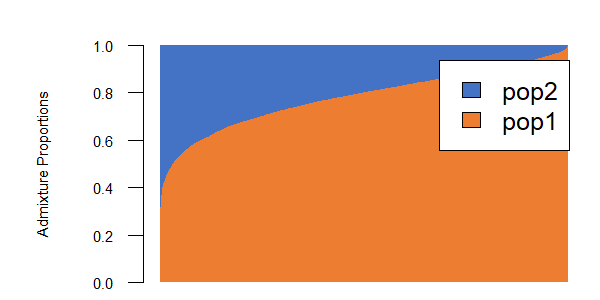
\includegraphics[width=0.7\textwidth]{figs/theorysims/sims_barplot}
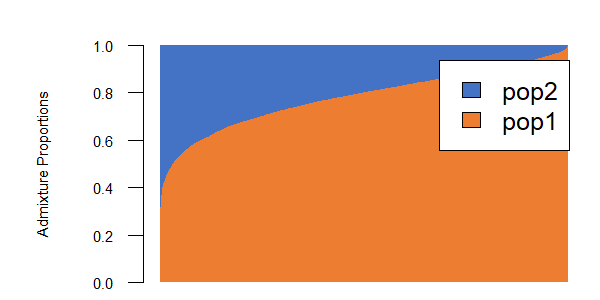
\includegraphics[width=0.7\textwidth]{figs/finalfigs/figS7_sims_barplot}
\caption{Barplot of simulated admixture proportions.}
\label{fig:barplot}
\end{figure}


In Figures \ref{fig:unadjust}, \ref{fig:pi}, and \ref{fig:pcs_gwas} we plot the effect size estimates from GWAS models that we observe in our simulation study, and compare these observed effect size estimates to the expected effect sizes based on our analytic results (Section \ref{sec:expectedbetas}), as well as the true effect sizes based on the data-generating mechanism (Section \ref{sec:datagen}). 
For all three types of models, we see a perfect correspondence between the observed effect sizes and the expected effect sizes provided in Section \ref{sec:expectedbetas}, validating our theoretical derivations.

Comparing the observed and expected effect sizes to the true effect sizes provides insight into the magnitude of bias that can be expected from each model. 
Figure \ref{fig:unadjust} presents results using the unadjusted GWAS model.
We see a departure between the true effect size (0) and the observed and expected effect sizes at the unlinked neutral variant (SNP 2), confirming that models that fail to adjust for ancestral heterogeneity can yield biased estimates of the effect size even when global ancestry does not have a direct effect on the trait ($\beta_\pi = 0$).

\begin{figure}[!htb]
\centering
%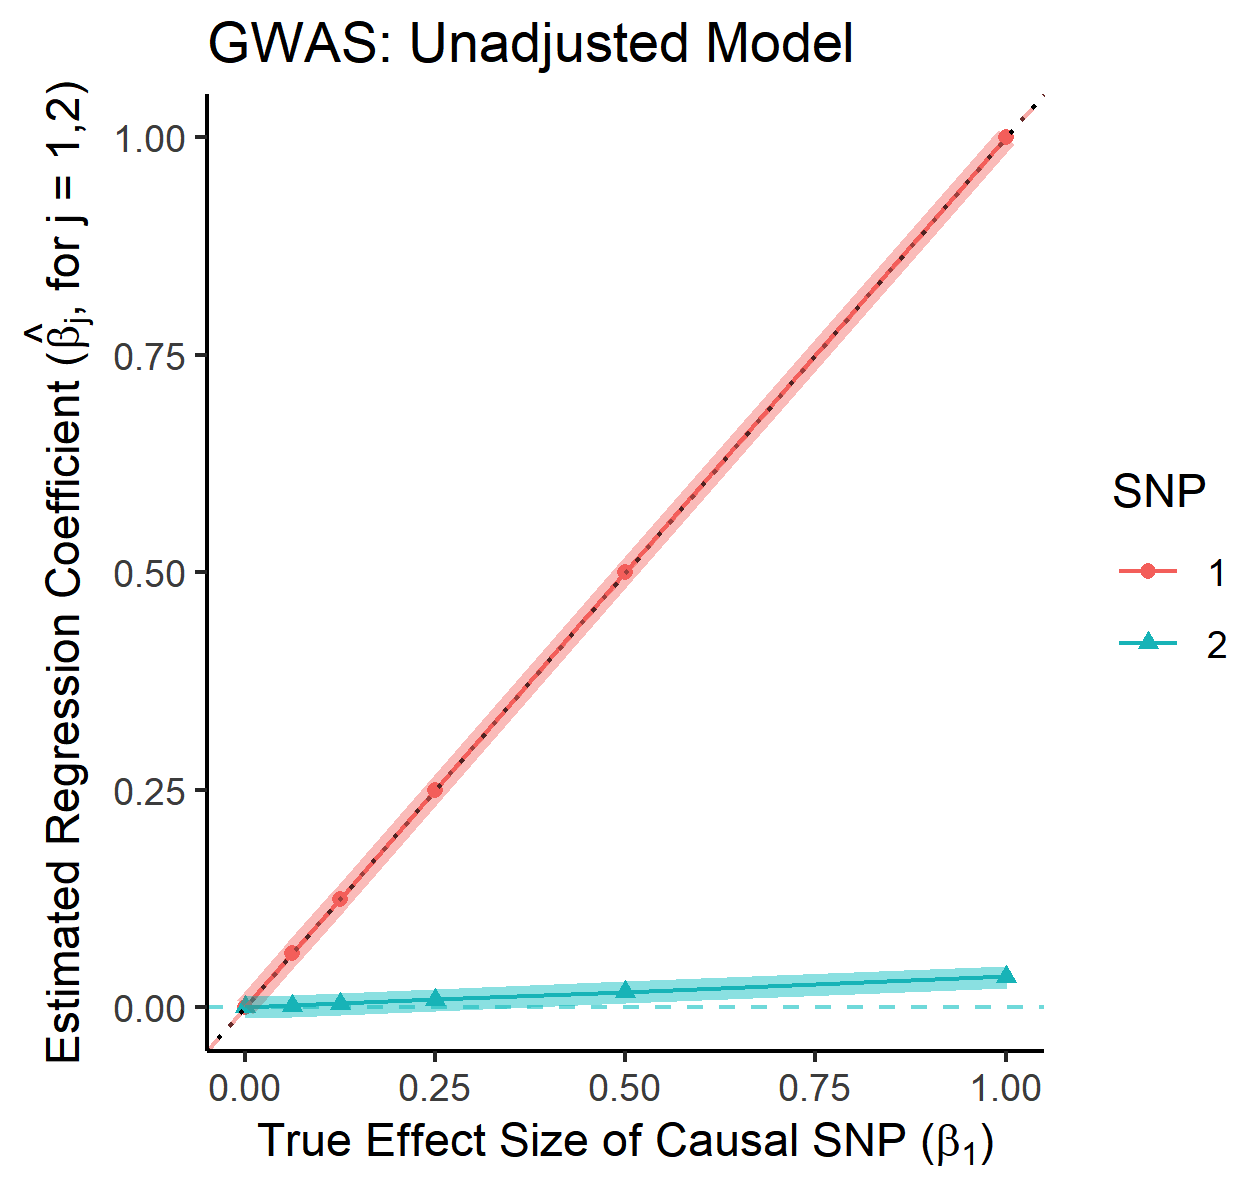
\includegraphics[width=0.55\textwidth]{figs/theorysims/sims_unadjusted}
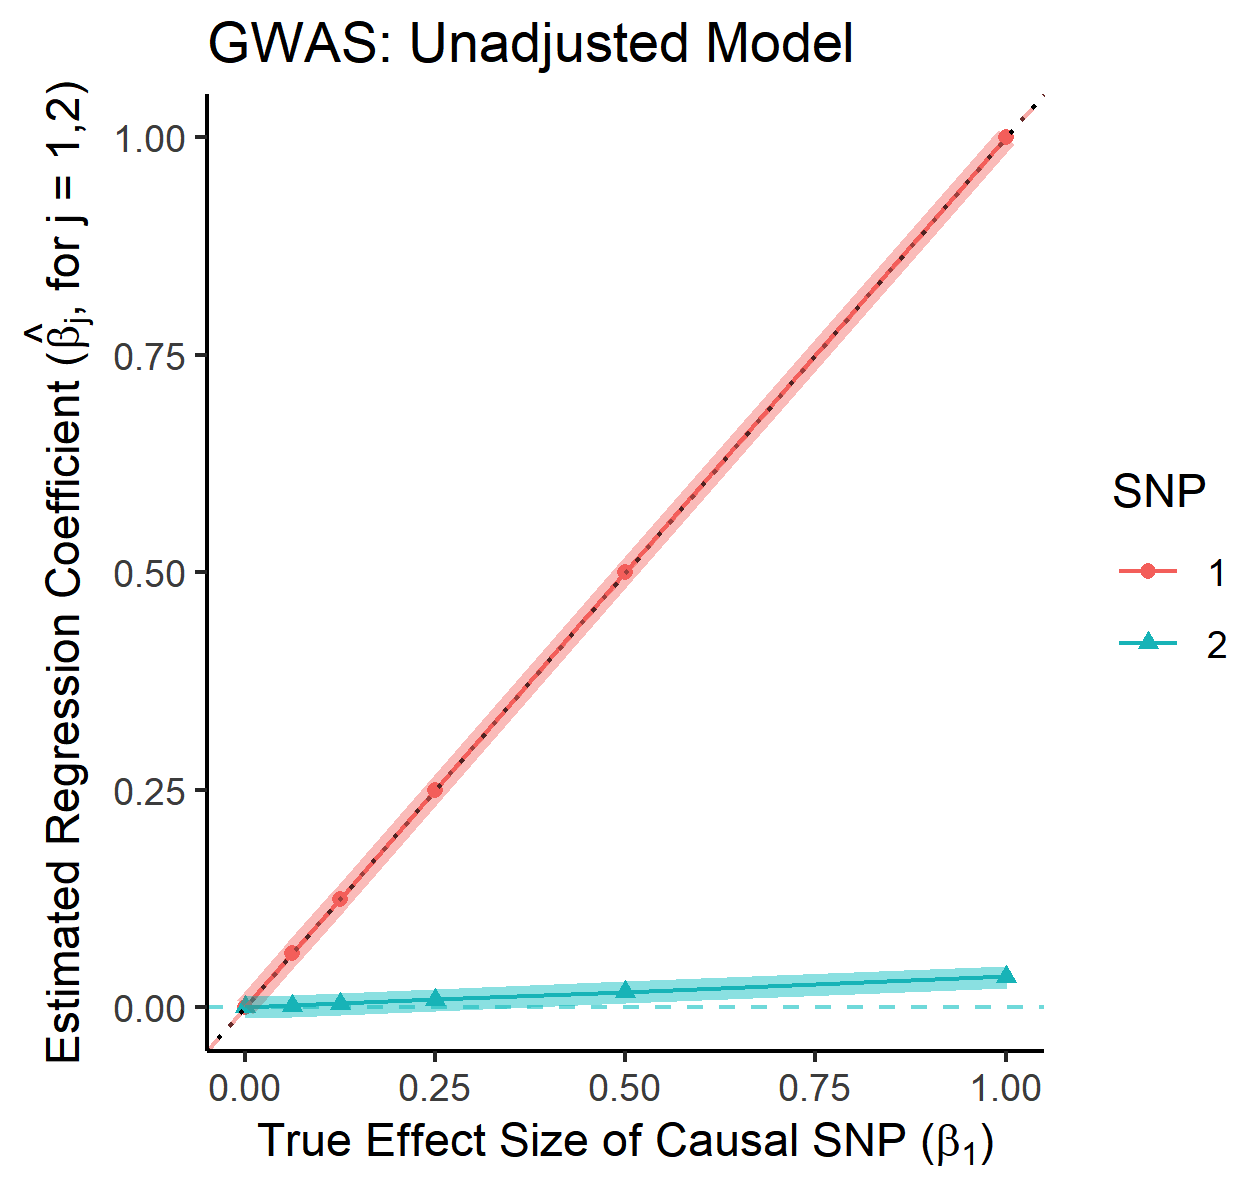
\includegraphics[width=0.55\textwidth]{figs/finalfigs/figS8_sims_unadjusted}
\caption[Observed versus expected and true effect sizes from unadjusted GWAS models.]%
{Comparison of observed, expected, and true effect sizes from unadjusted GWAS models applied to simulated data. Observed effect sizes are represented by the thin solid lines with points (\textcolor{red}{red} with dots = SNP 1, \textcolor{blue}{blue} with triangles = SNP 2). 
Expected effect sizes from Section \ref{sec:expectedbetas} are represented by the wider and faintly colored solid lines (\textcolor{red}{red} = SNP 1, \textcolor{blue}{blue} = SNP 2).
True effect sizes are represented by the dashed lines (\textcolor{red}{red} = SNP 1, \textcolor{blue}{blue} = SNP 2).
The $y = x$ line is also provided for reference (dotted black line).}
%The perfect correspondence between the observed and expected effect sizes validates our theoretical results. 
%For SNP 2, we see a departure between the true effect size (0) and the observed and expected effect sizes, illustrating the bias that arises if we fail to adjust for ancestral heterogeneity.}
\label{fig:unadjust}
\end{figure}

In Figure \ref{fig:pi}, we consider the case of a GWAS model that adjusts for ancestral heterogeneity by including the true admixture proportions as a covariate.
In this case, we see a perfect correspondence between the observed, expected, and true effect sizes for both the causal and unlinked neutral variants. 
This confirms, as our theory suggests, that models that appropriately adjust for ancestral heterogeneity will yield unbiased estimates of variant effect sizes (i.e., $E[\hat\beta_j] = \beta_j$).


\begin{figure}[!htb]
\centering
%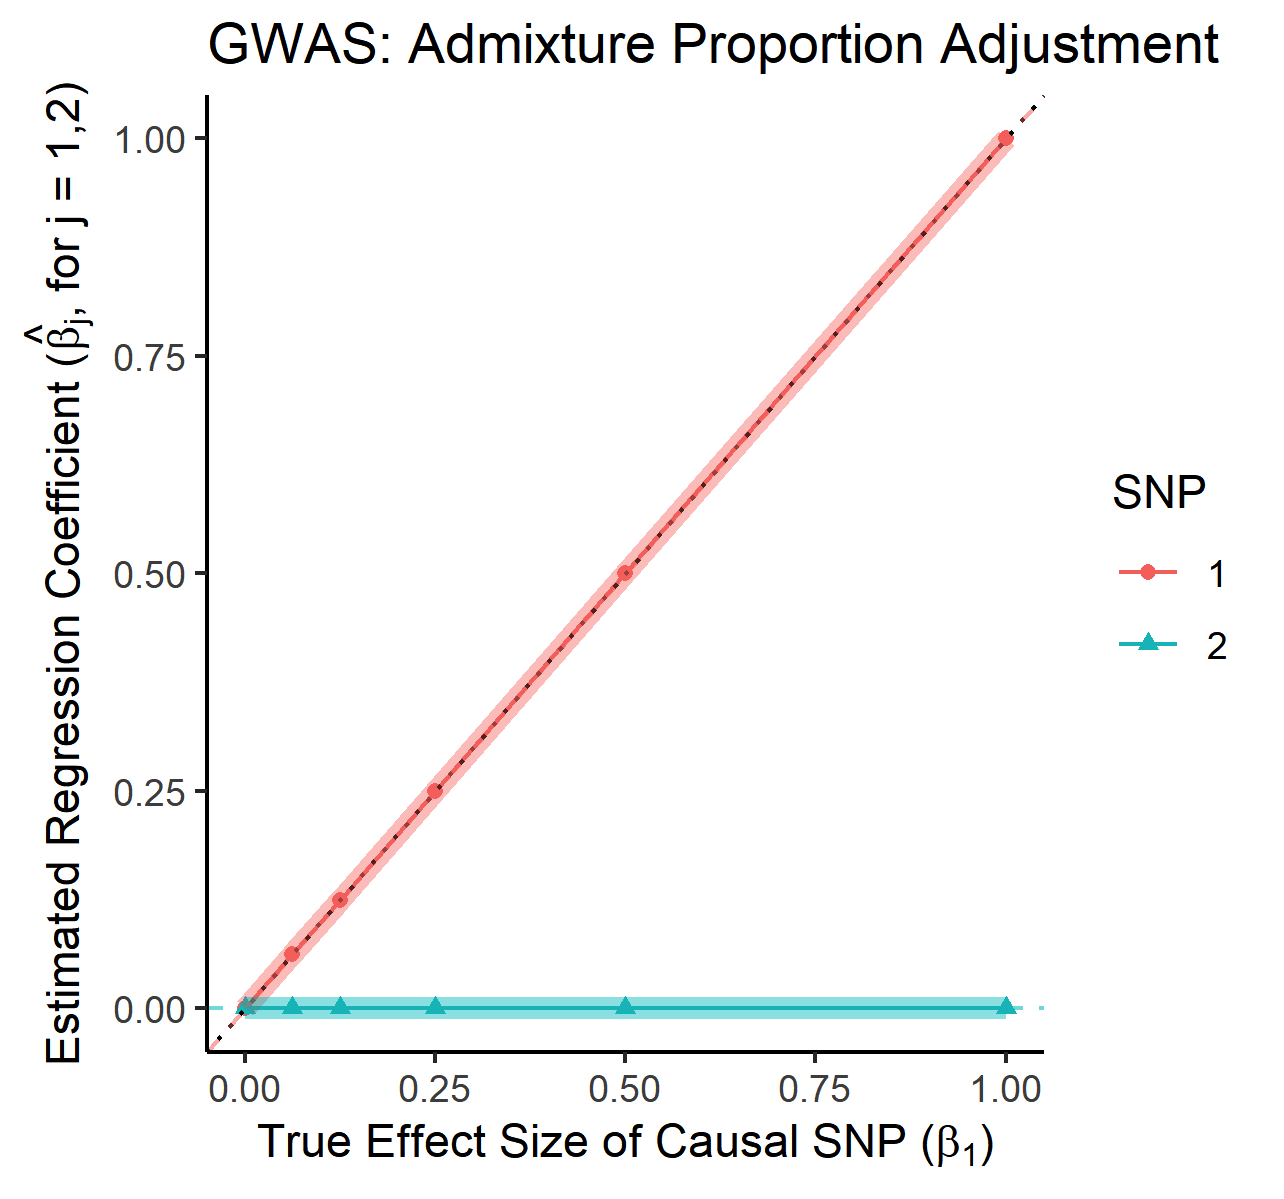
\includegraphics[width=0.6\textwidth]{figs/theorysims/sims_pi}
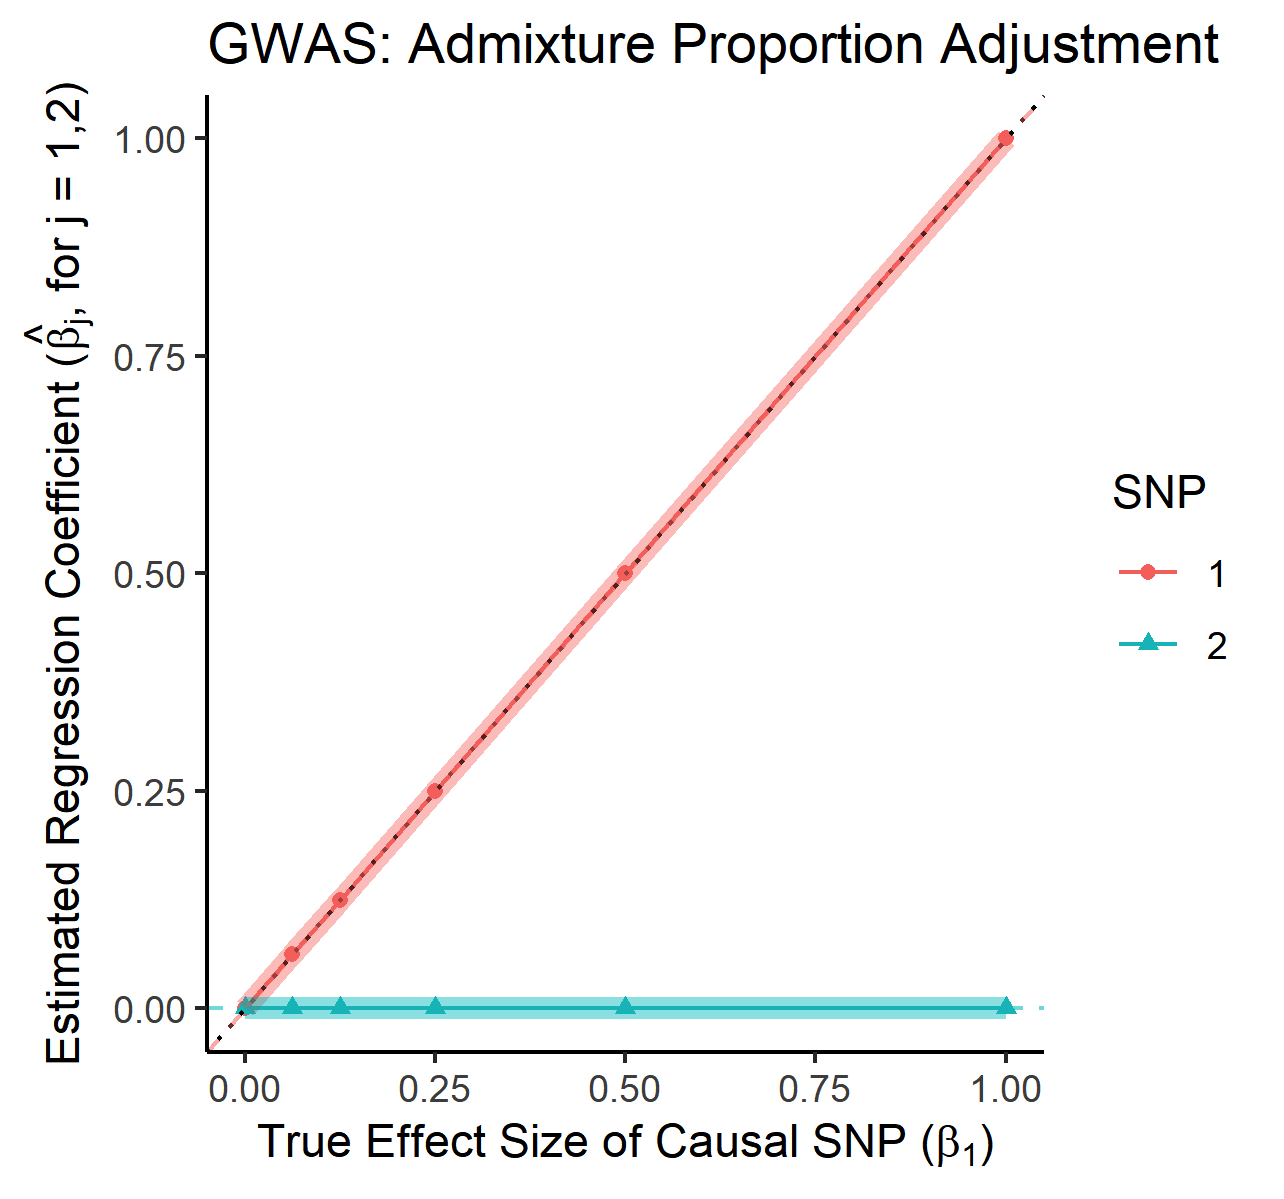
\includegraphics[width=0.6\textwidth]{figs/finalfigs/figS9_sims_pi}
\caption[Observed versus expected and true effect sizes from admixture proportion adjusted GWAS models.]%
{Comparison of observed, expected, and true effect sizes from GWAS models adjusting for admixture proportions in simulated data. 
Observed effect sizes  are represented by the thin solid lines with points (\textcolor{red}{red} with dots = SNP 1, \textcolor{blue}{blue} with triangles = SNP 2). 
Expected effect sizes  from Section \ref{sec:expectedbetas} are represented by the wider and faintly colored solid lines (\textcolor{red}{red} = SNP 1, \textcolor{blue}{blue} = SNP 2).
True effect sizes are represented by the dashed lines (\textcolor{red}{red} = SNP 1, \textcolor{blue}{blue} = SNP 2).
The $y = x$ line is also provided for reference (dotted black line).}
%The perfect correspondence between the observed and expected effect sizes again validates our theoretical results, and the correspondence between these and the true effect size confirm that results will be unbiased if GWAS models appropriately adjust for ancestral heterogeneity.  }
\label{fig:pi}
\end{figure}


Figure \ref{fig:pcs_gwas} illustrates the impact of adjusting for a principal component that captures local genomic features (in this case, the genotype of variants 1 and 2) instead of global ancestry. 
Specifically, the second PC was generated according to the equation $z_1 g_{i1} + z_2 g_{i2} + N(0, 0.25^2)$ for scalars $z_1, z_2$.
Although the effect sizes estimates for variant 1 are unbiased across all simulation settings, confirming our theoretical result that $E[\hat\beta_1] = \beta_1$ (see Section \ref{sec:expectedbetas}), we see that the observed and expected effect sizes for SNP 2 often deviate from the truth. 
The only situations in which effect size estimates for this neutral unlinked variant are unbiased (i.e., $E[\hat\beta_2] = \beta_2 = 0$) are when the PC is not actually affected by the causal variant (i.e., $z_1 = 0$) or when the PC is not affected by the neutral variant (i.e., $z_2 = 0$). 
In other words, as long as the extraneous PC captures the genotypes of both the causal variant and the unlinked neutral variant, we see that effect sizes are biased away from zero at this neutral variant.
The magnitude of this bias increases with the strength of the relationship between the variants and the PC (i.e., as we increase $z_1$ and/or $z_2$).

\begin{figure}[!htb]
\centering
%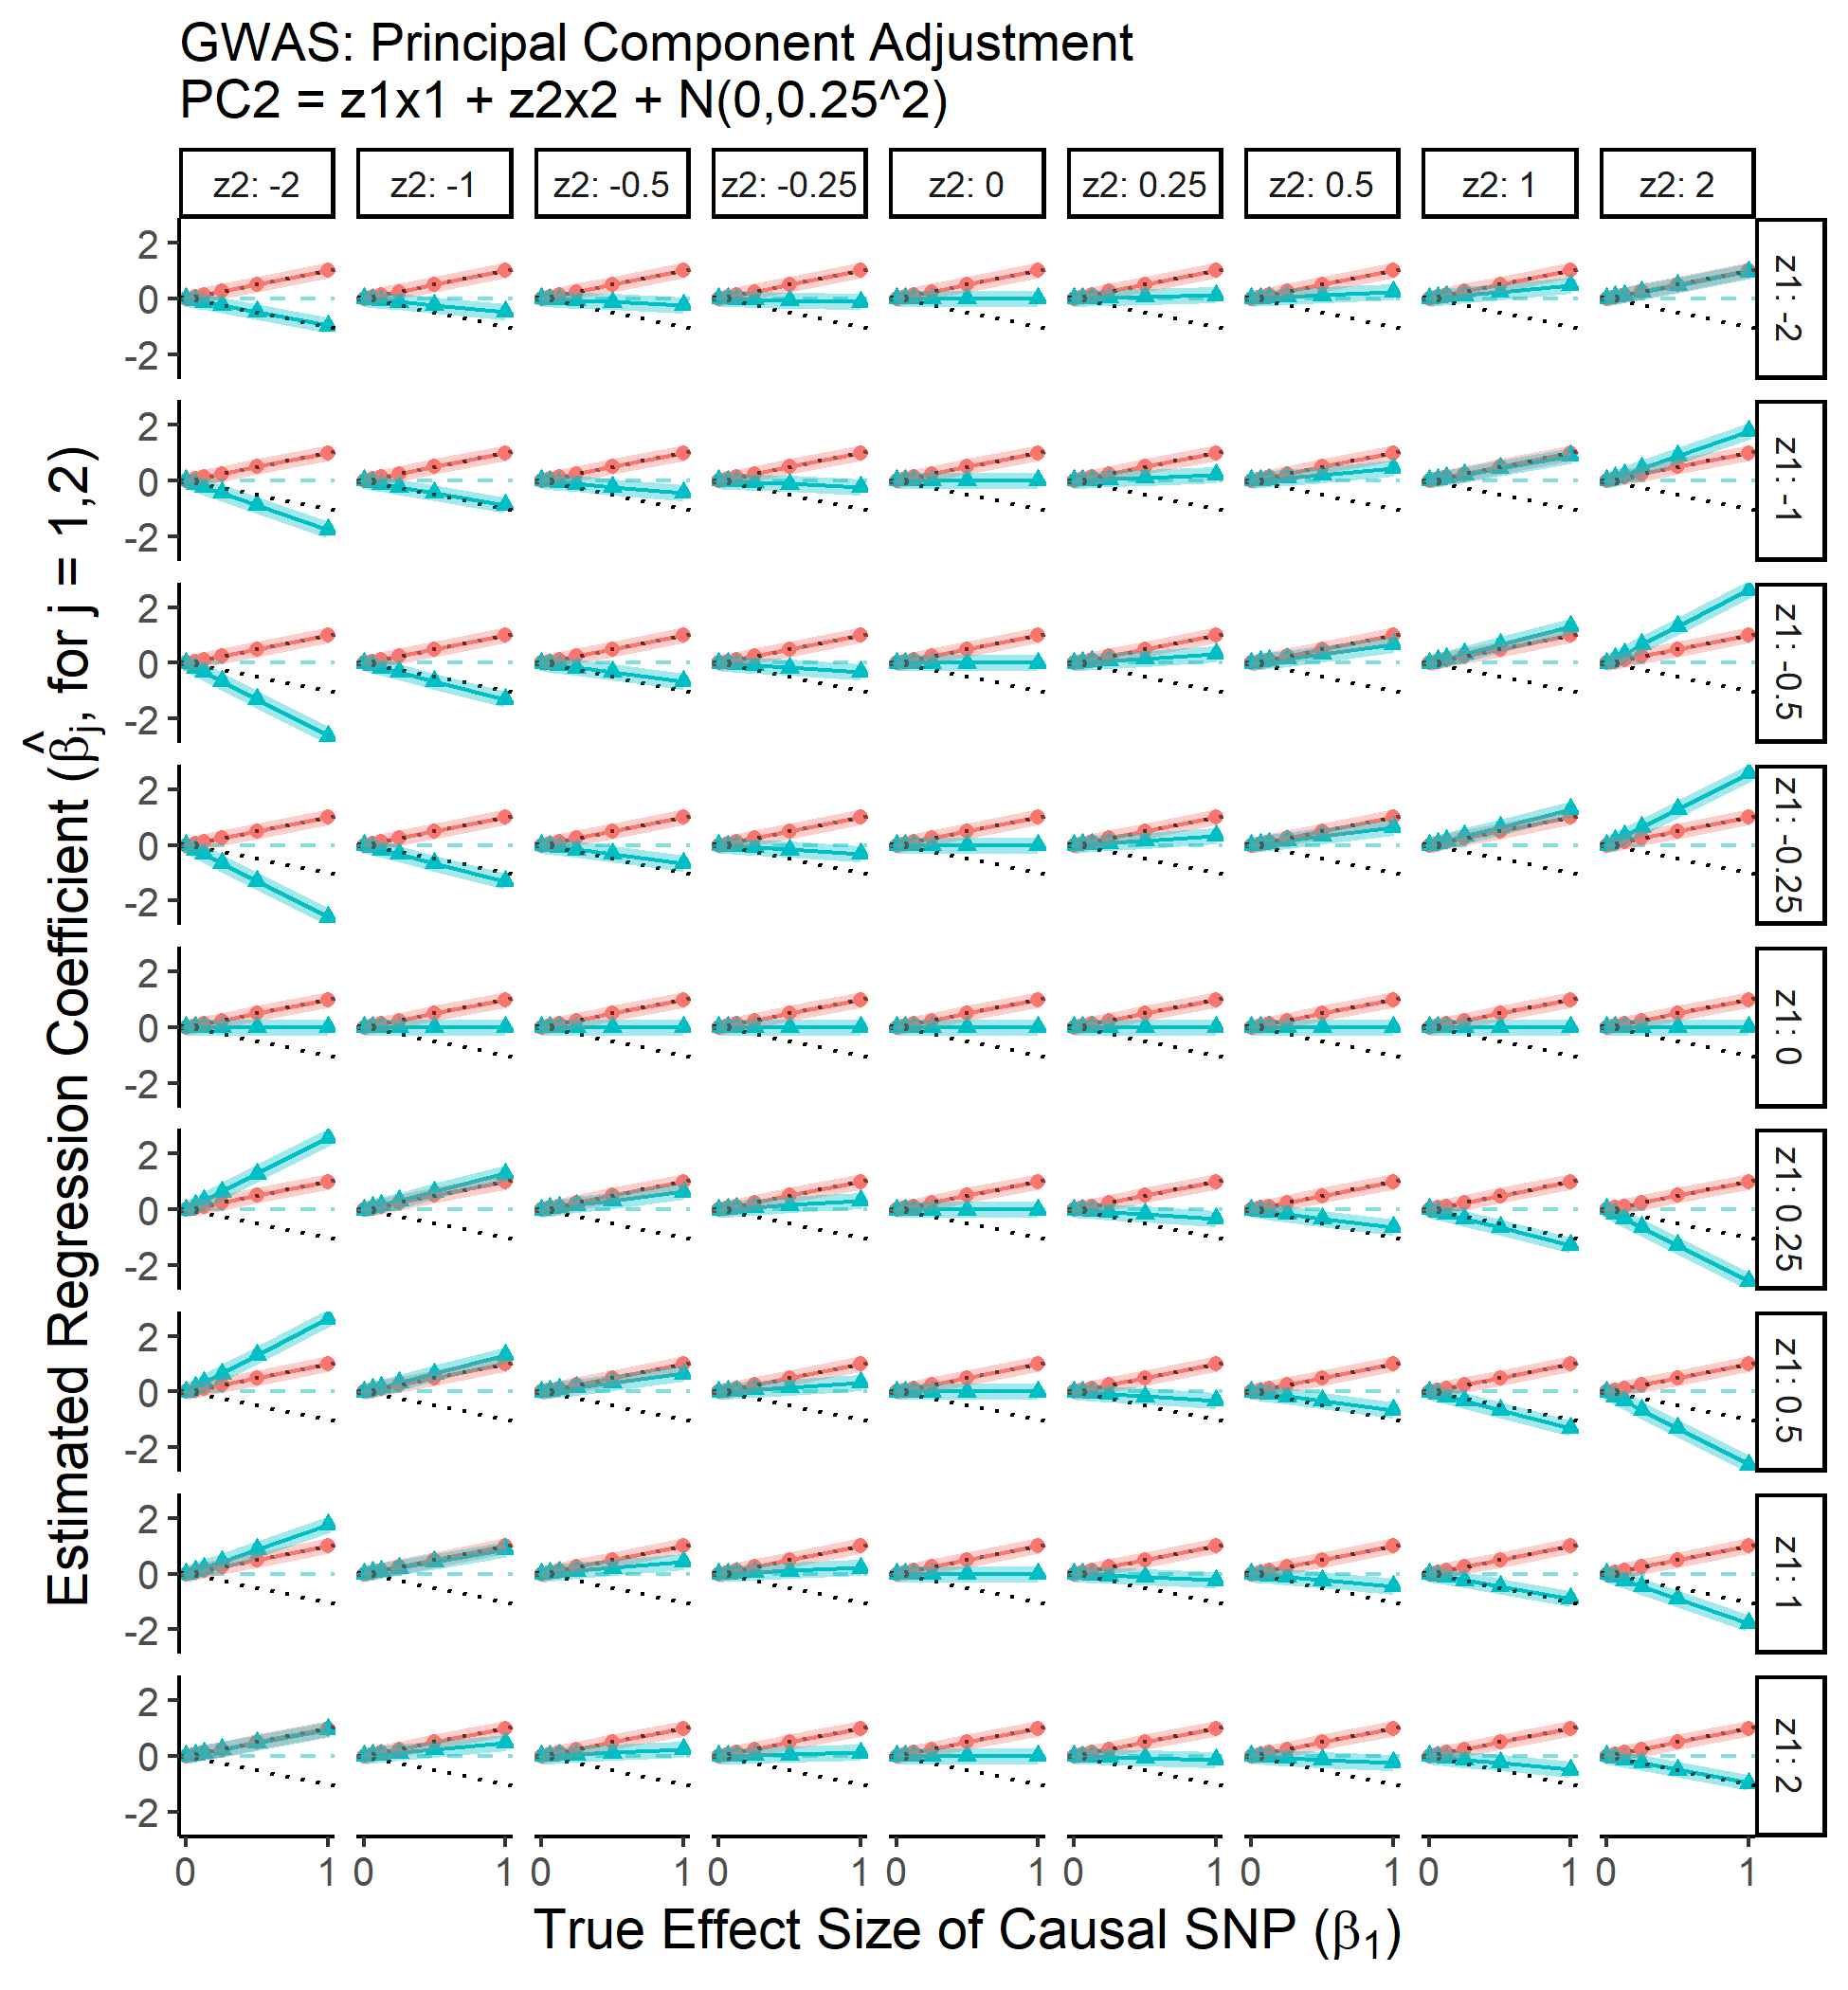
\includegraphics[width=0.98\textwidth]{figs/theorysims/sims_pcs_gwas}
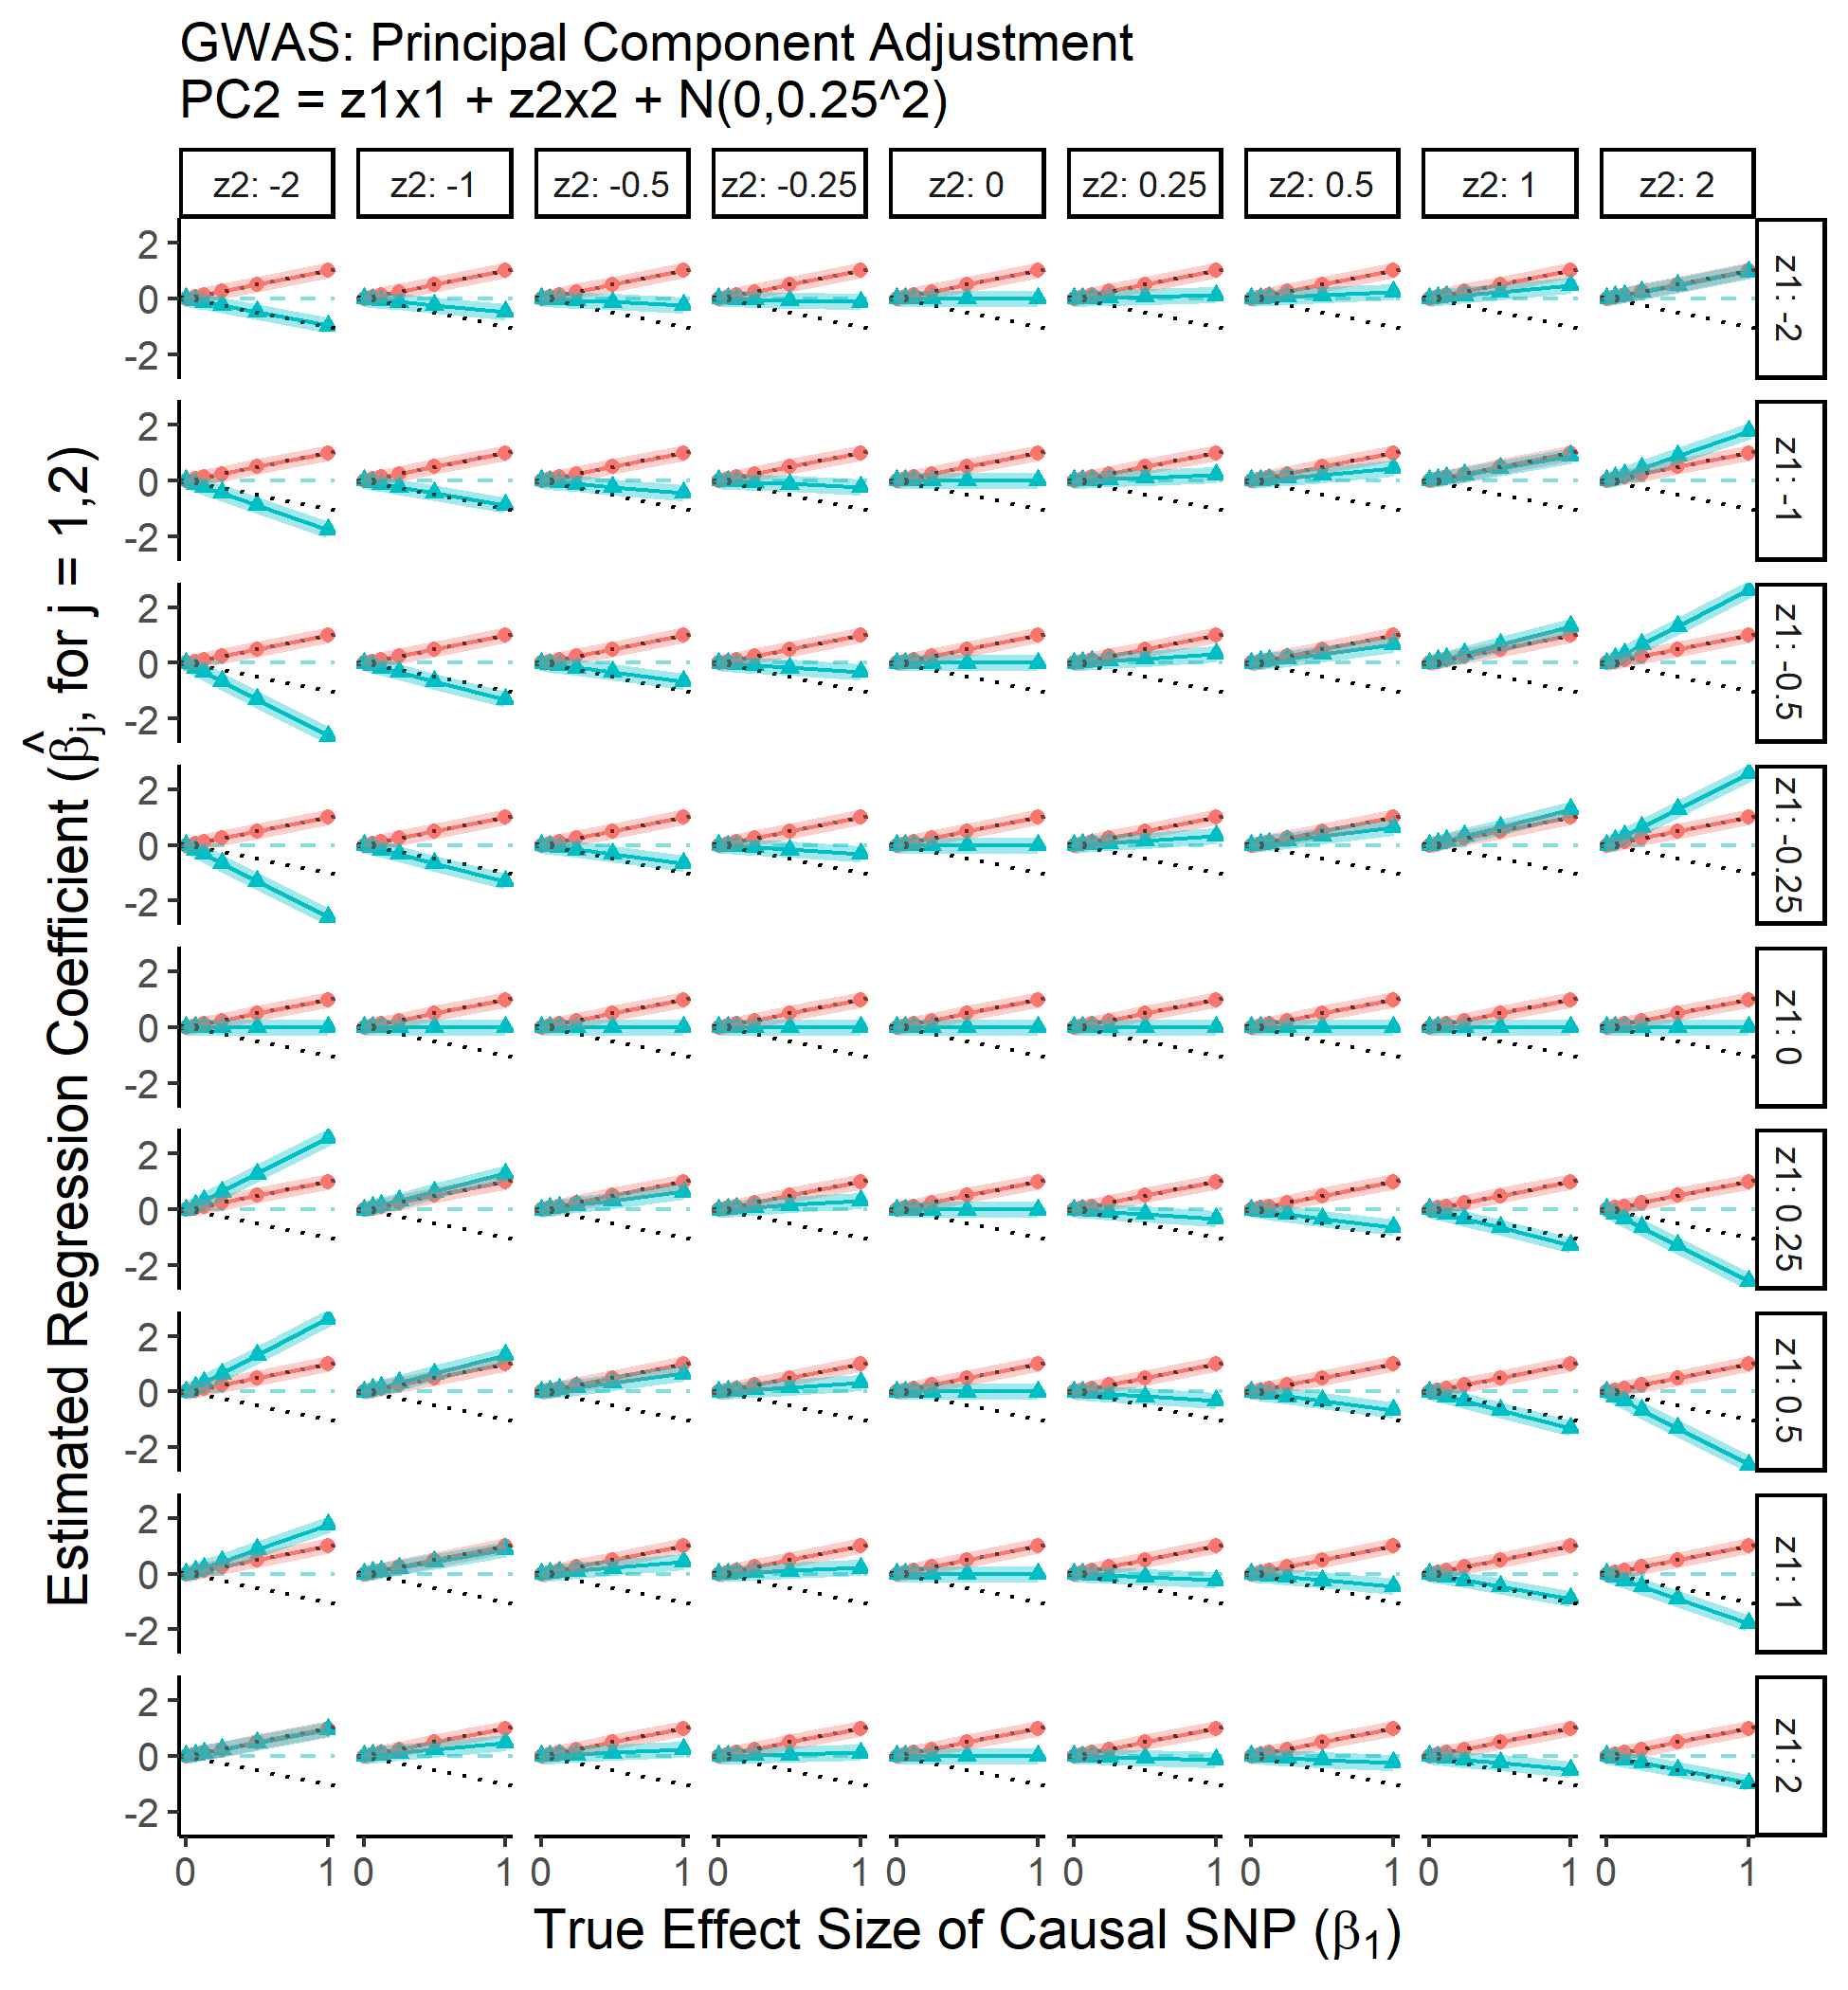
\includegraphics[width=0.98\textwidth]{figs/finalfigs/figS10_sims_pcs_gwas}
\caption[Observed versus expected and true effect sizes from principal component adjusted GWAS models.]%
{Comparison of observed, expected, and true effect sizes from GWAS models adjusting for two principal components. 
The first PC captures global ancestry, but the second PC was generated according to the equation $z_1 g_{i1} + z_2 g_{i2} + N(0, 0.25^2)$, changing the scalars $z_1,z_2$ in each panel.
Observed effect sizes  are represented by the thin solid lines with points (\textcolor{red}{red} with dots = SNP 1, \textcolor{blue}{blue} with triangles = SNP 2). 
Expected effect sizes  are represented by the wider and faintly colored solid lines (\textcolor{red}{red} = SNP 1, \textcolor{blue}{blue} = SNP 2).
True effect sizes are represented by the dashed lines (\textcolor{red}{red} = SNP 1, \textcolor{blue}{blue} = SNP 2).
The $y = x$ line is also provided for reference (dotted black line).}
\label{fig:pcs_gwas}
\end{figure}

%\begin{figure}
%\centering
%% ----- switch this before including in dissertation
%\includegraphics[width=0.9\textwidth]{chap5/figs/sims_pcs_amap}
%%\includegraphics[width=0.9\textwidth]{figs/sims_pcs_amap}
%% ----- switch this before including in dissertation
%\caption[Observed versus expected and true effect sizes from principal component adjusted admixture mapping models.]%
%{Observed versus expected and true effect sizes from principal component adjusted admixture mapping models. \par \small Each panel represents a different simulation setting where the second PC was generated according to the equation $z_1 g_{i1} + z_2 g_{i2} + N(0, 0.25^2)$, changing the scalars $z_1,z_2$ in each panel.  Observed effect sizes  = solid lines with points (\textcolor{red}{red} with dots = SNP 1, \textcolor{blue}{blue} with triangles = SNP 2). 
%Expected effect sizes  = wider and faintly colored solid lines (\textcolor{red}{red} = SNP 1, \textcolor{blue}{blue} = SNP 2).
%True effect sizes = dashed lines (\textcolor{red}{red} = SNP 1, \textcolor{blue}{blue} = SNP 2).
%The $y = x$ line is also provided for reference (dotted black line).}
%\label{fig:pcs_amap}
%\end{figure}


\section{Additional Simulations using  TOPMed Data}
\label{sec:topmedsims}

We also performed simulations using whole genome sequence data from the Trans-Omics for Precision Medicine Project to further connect our theoretical results to the findings, presented in the main paper, from our simulation study using WHI SHARe genotype data.
For each individual, we simulated a quantitative trait that depended only on their genotype at a single variant on chromosome 8. 
We also constructed two ``fake" principal components.
The first PC was set equal to the estimated African admixture proportion (see Methods). 
The second PC was generated such that it depended on the genotype at this same causal variant, as well as another variant on chromosome 6.
Figure \ref{fig:corr-fake} shows that we see similar patterns in the correlation between this PC and genotypes as we did with real PCs (calculated without strict LD-based pruning) in WHI SHARe, TOPMed JHS, and TOPMed COPDGene African Americans. 
These PC-genotype correlation plots clearly show---as we know to be true, by design---that the second PC is driven by variants on two chromosomes (6 and 8) rather than detecting genome-wide ancestry. 

\begin{figure}[!htb]
\centering
%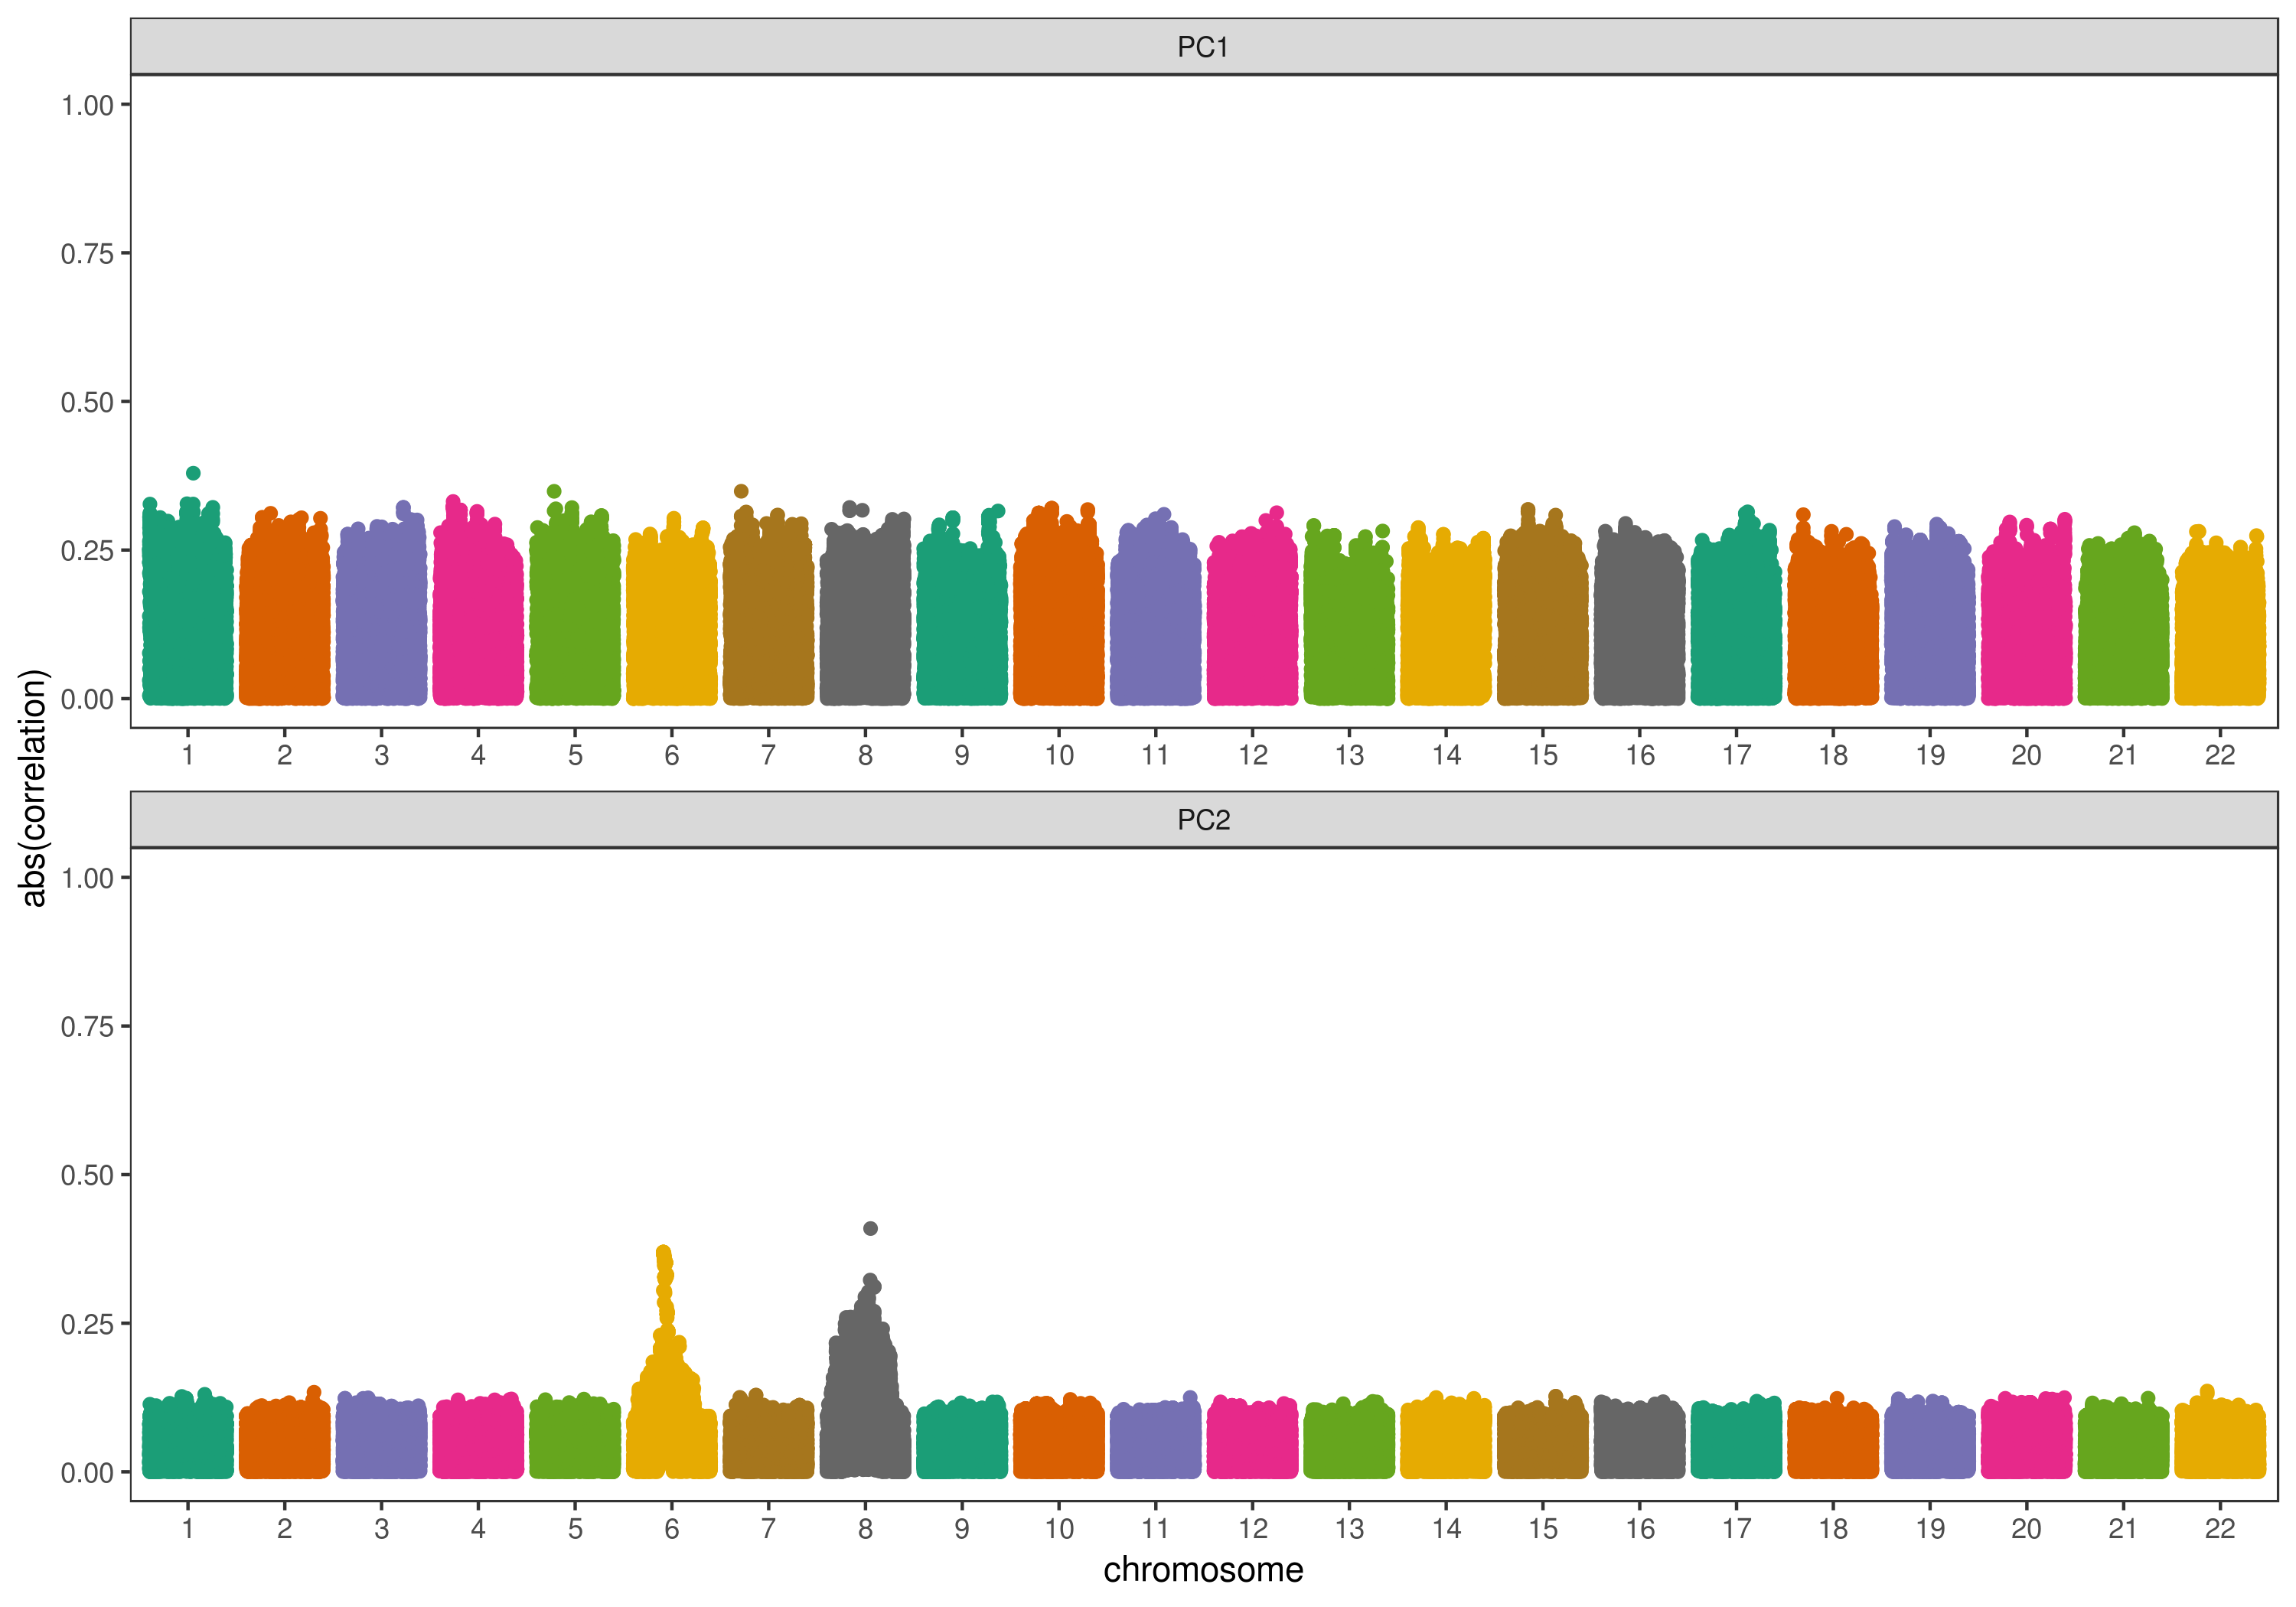
\includegraphics[width=\textwidth]{figs/fakepcs/fake_pcs_corr_1}
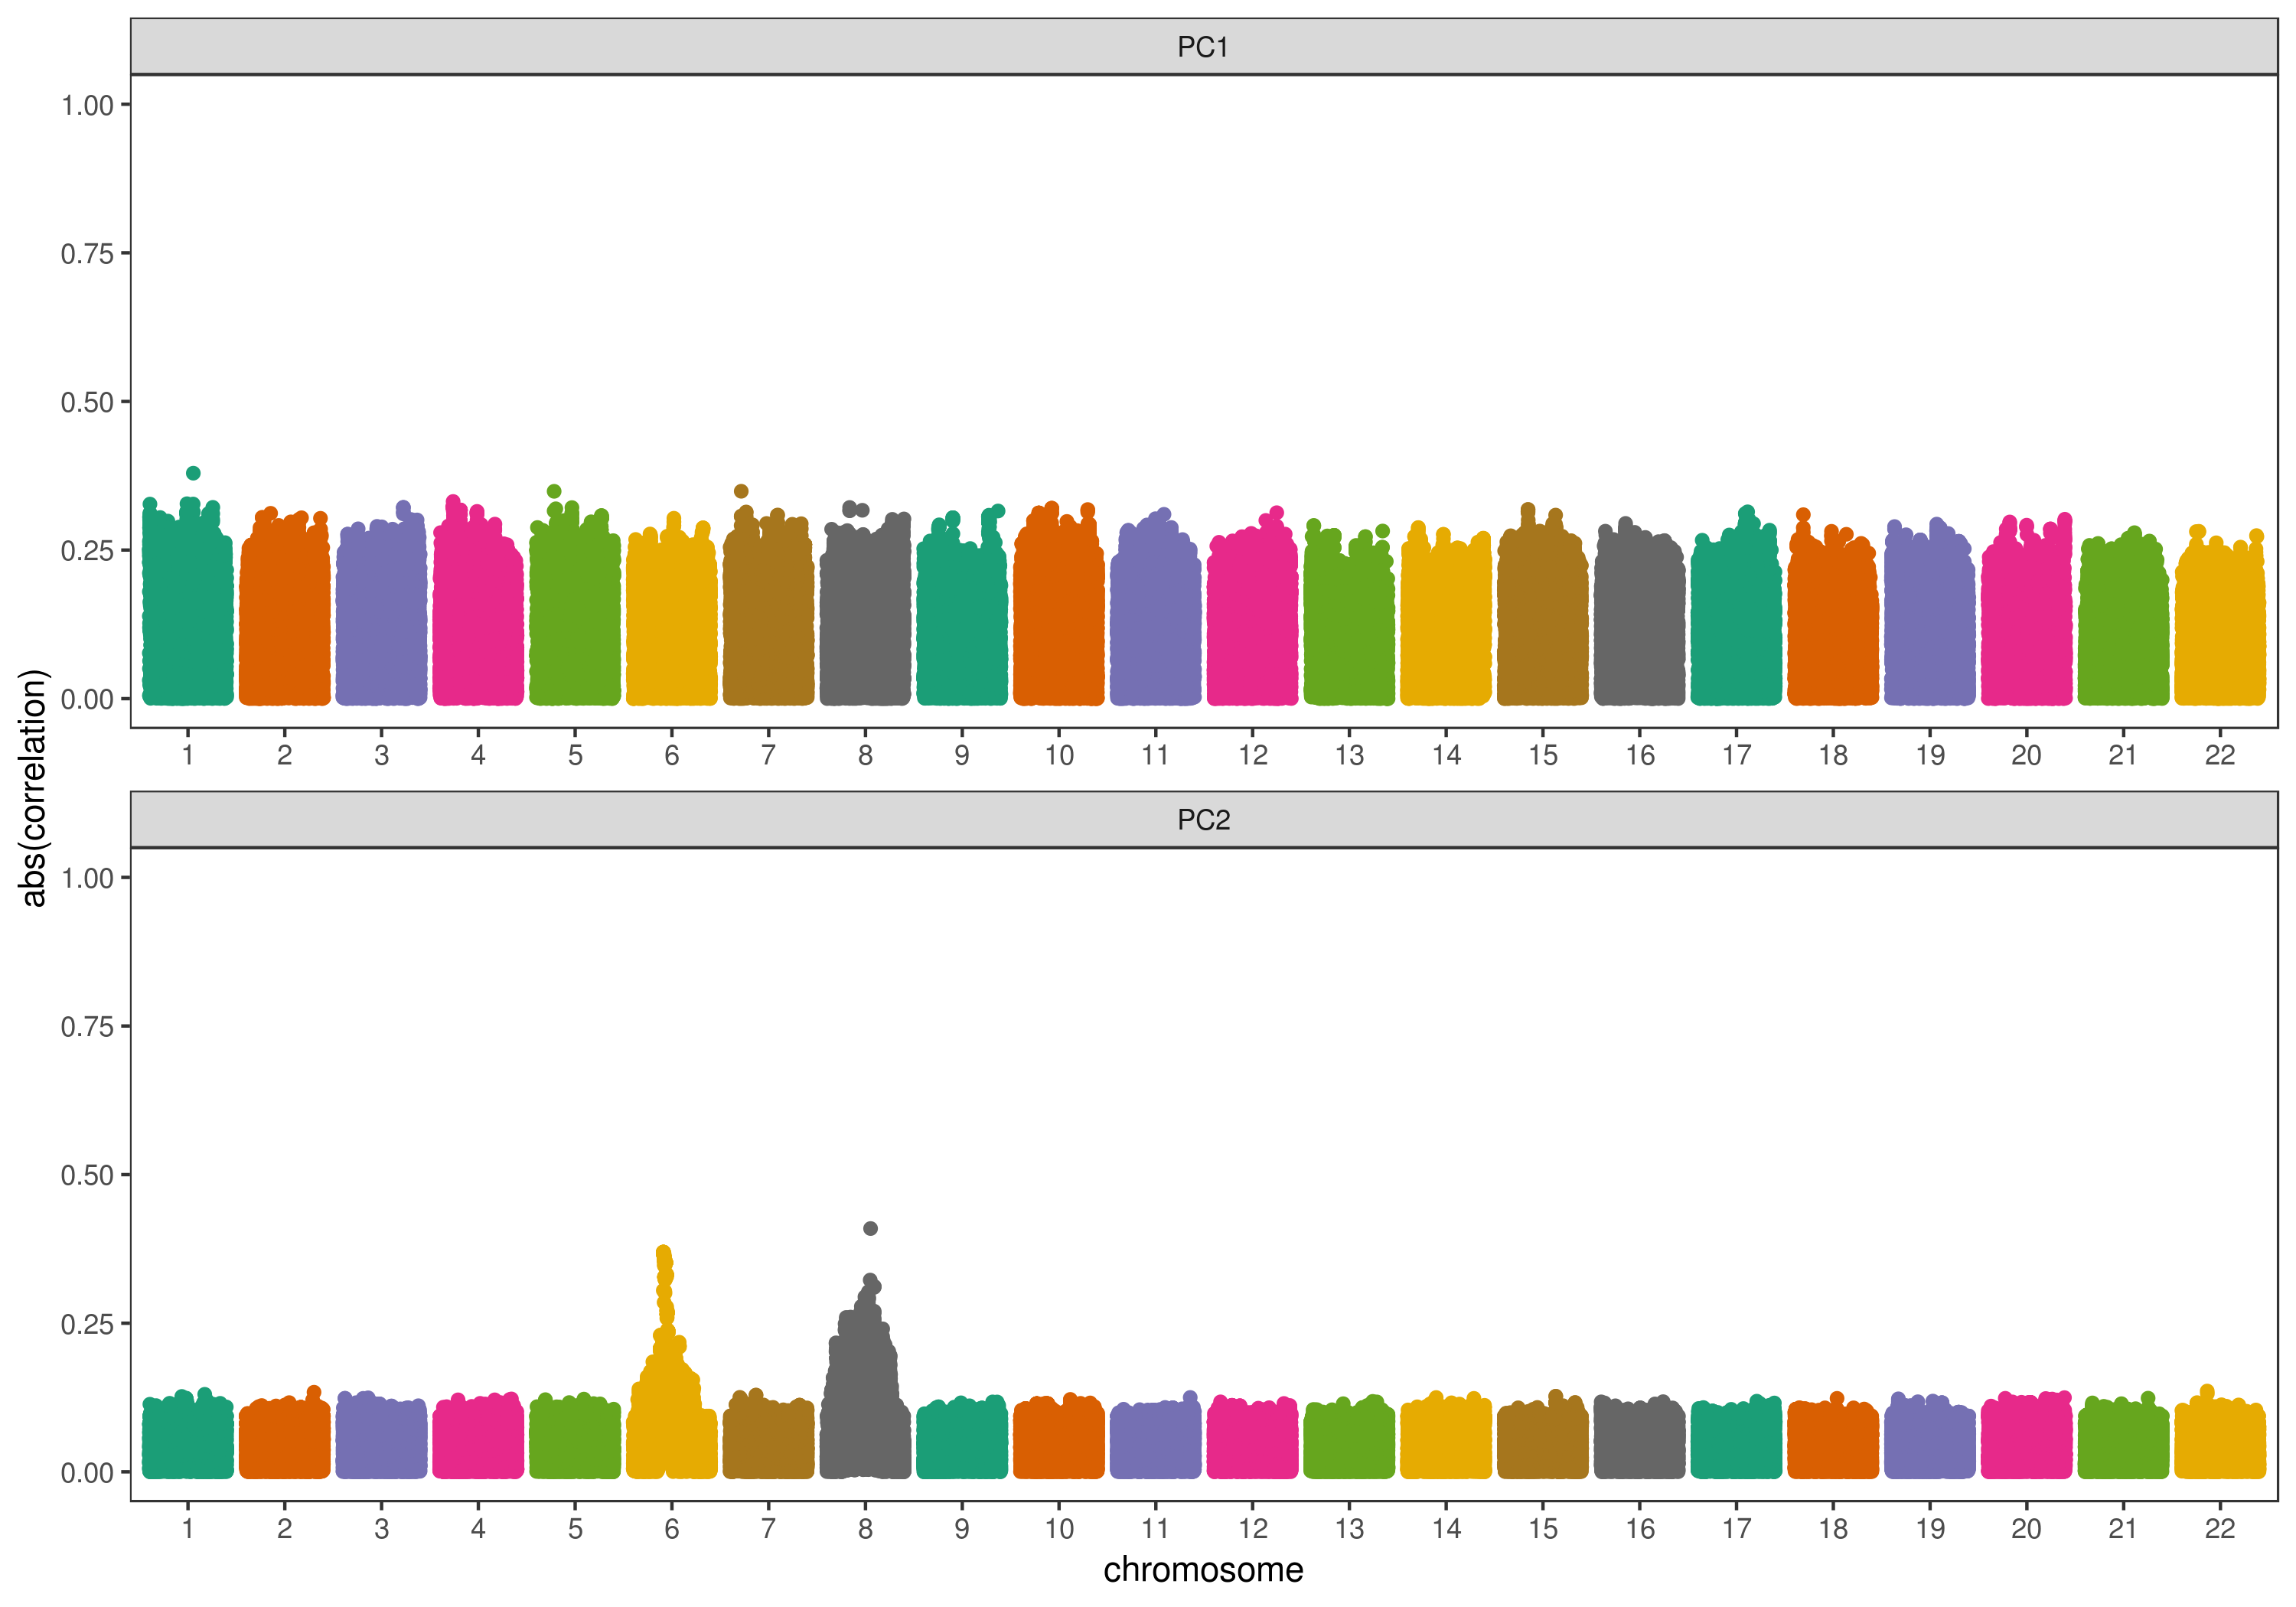
\includegraphics[width=\textwidth]{figs/finalfigs/figS11_fake_pcs_corr_1}
\caption[Correlation between fake PCs and genotypes in TOPMed JHS.]{Correlation between fake PCs (i.e., PCs that were constructed such that the first captures genetic ancestry but the second captures genotype at two variants on chromosomes 6 and 8) in TOPMed JHS African Americans. Each panel plots the absolute value of the correlation between principal components and genotypes (on the y-axis) versus the position along the genome (x-axis).  Panels are organized vertically according to which PC is being investigated (1, 2). Peaks in this plot indicate that a variant has a larger \textit{loading}, i.e., a larger contribution to that principal component.}
\label{fig:corr-fake}
\end{figure}


We then investigated the impact of including this extraneous PC in GWAS models. 
Our results again mirror the patterns observed in our WHI SHARe simulations.
Figure \ref{fig:manh-fake} presents Manhattan plots from a single simulation replicate, comparing results from a model that adjusted for just the first principal component (top panel) versus a model that adjusted for both PCs (bottom panel).
In both cases, we see a genome-wide significant association on chromosome 8 --- the location of the true causal variant.
However, in the case of the model adjusting for two PCs, we also see a spurious association on chromosome 6 --- the location of the second variant that contributes to the second principal component.
The second PC plays the role of a collider variable in this setting, and adjusting for it has induced a spurious association.
It is worth noting that the quantile-quantile (QQ) plots and inflation factors for these two analyses are indistinguishable (Figure \ref{fig:qq-fake}), so those tools alone are not sufficient for detecting this issue of collider bias caused by including PCs that capture multiple local genomic features, rather than genetic ancestry.

\begin{figure}[!htb]
\centering
%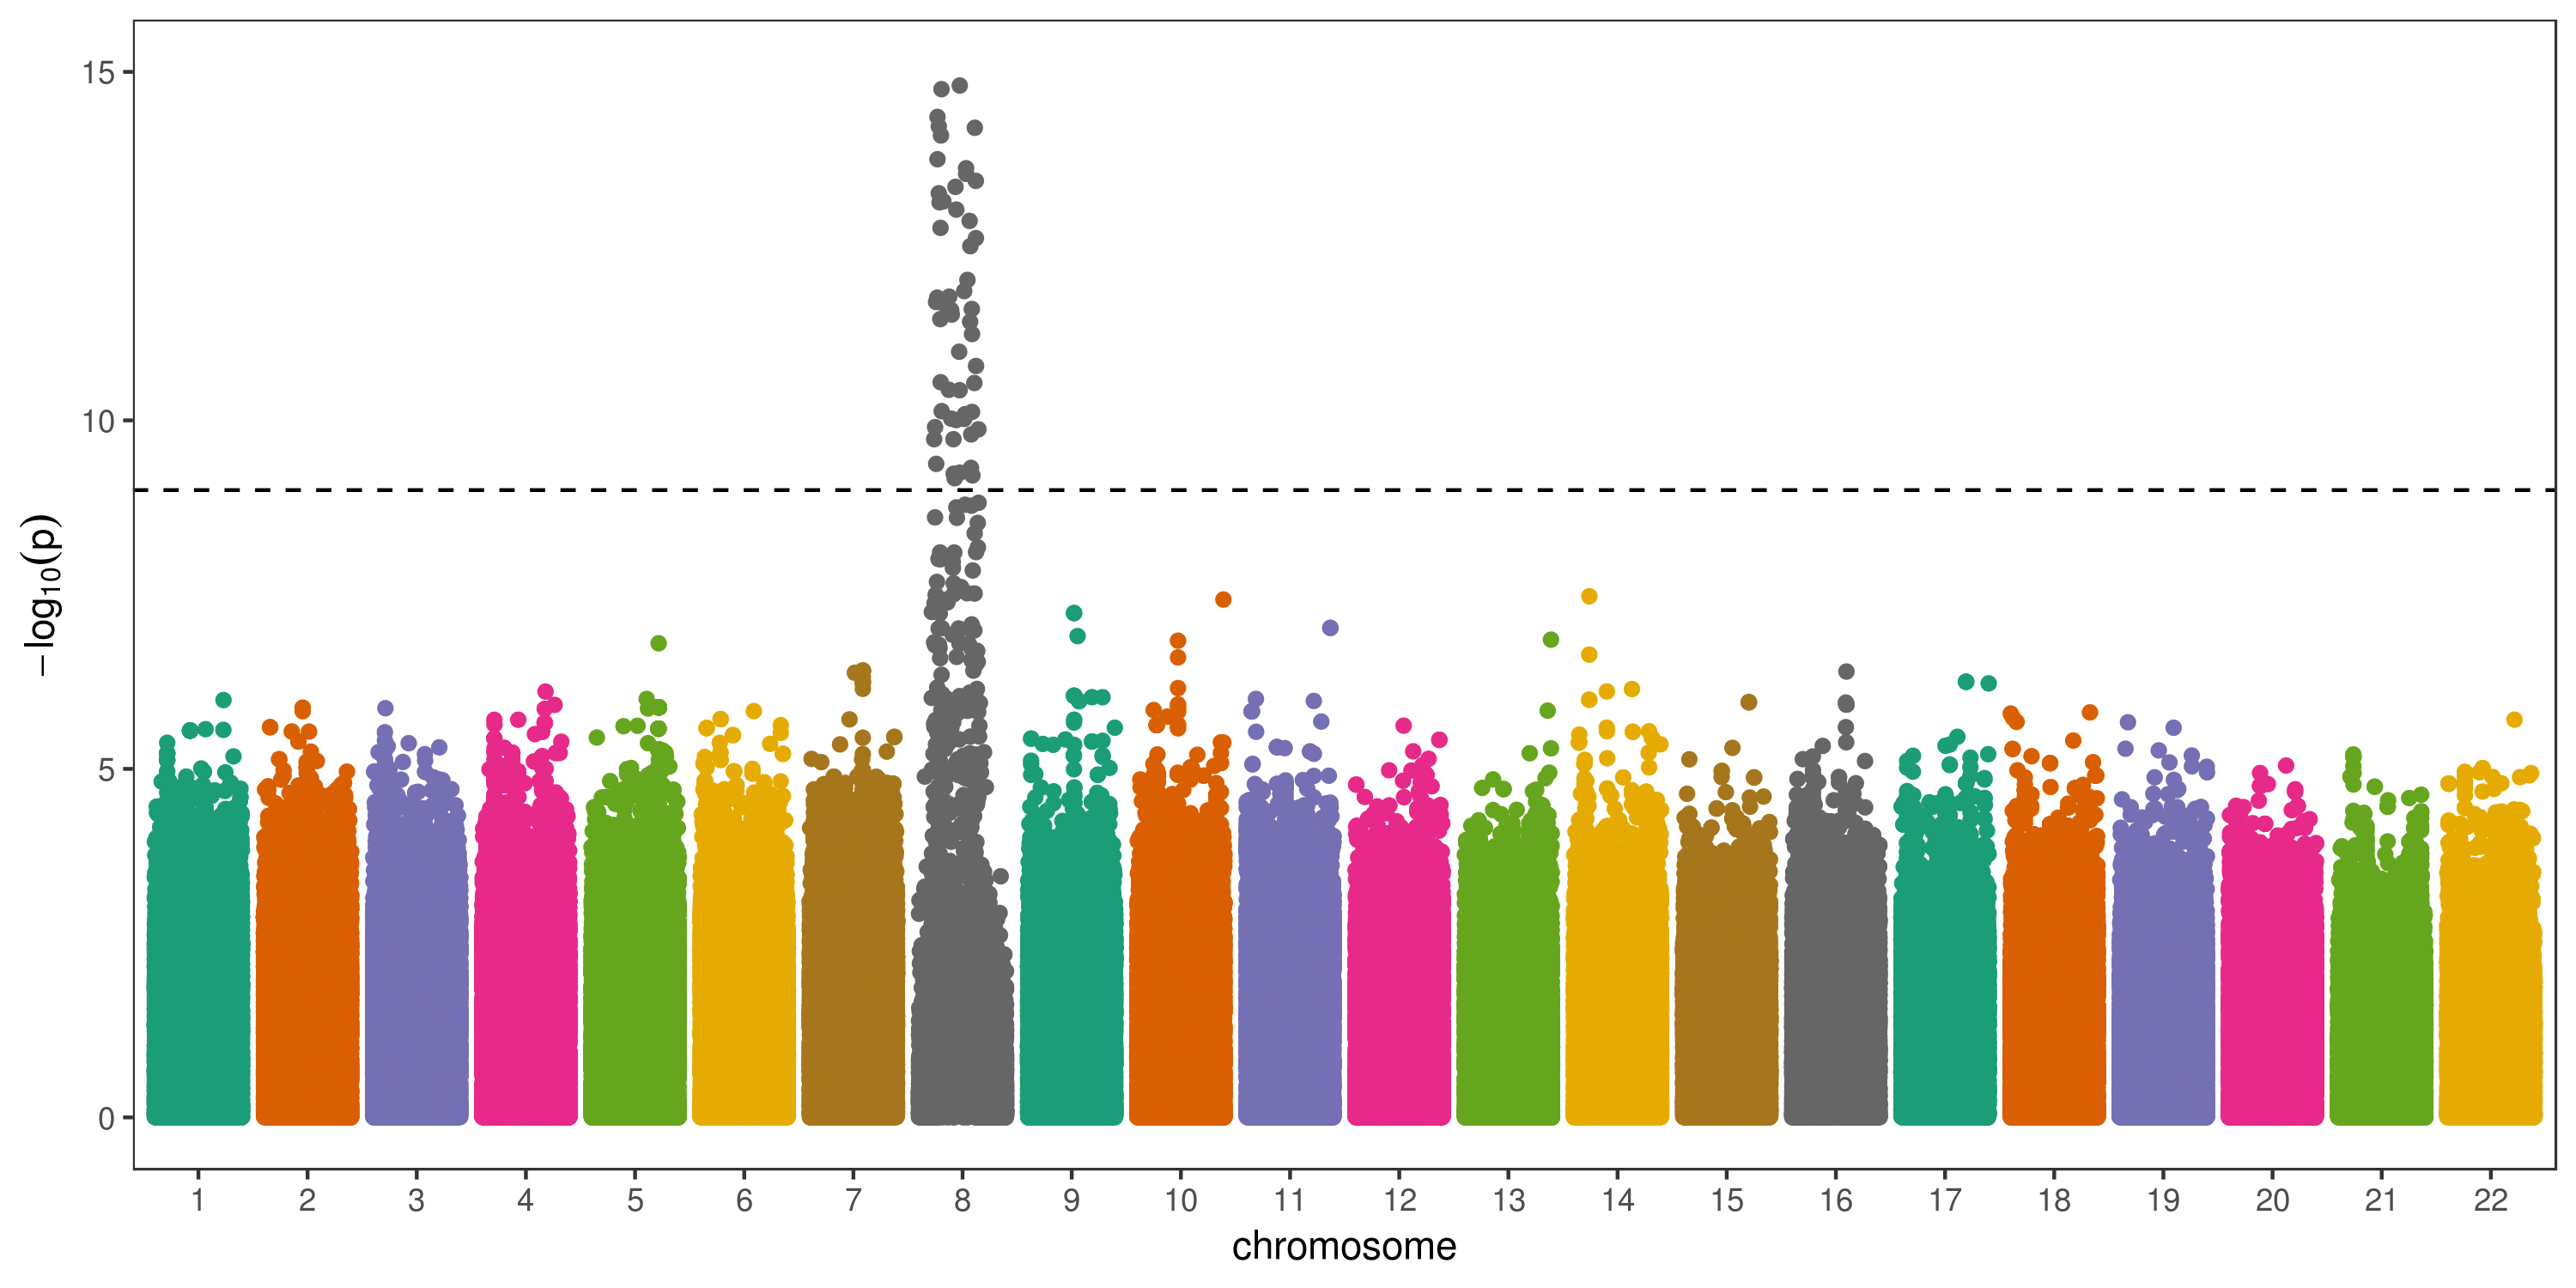
\includegraphics[width=\textwidth]{figs/fakepcs/beta2_1pcs_fake_manh}
%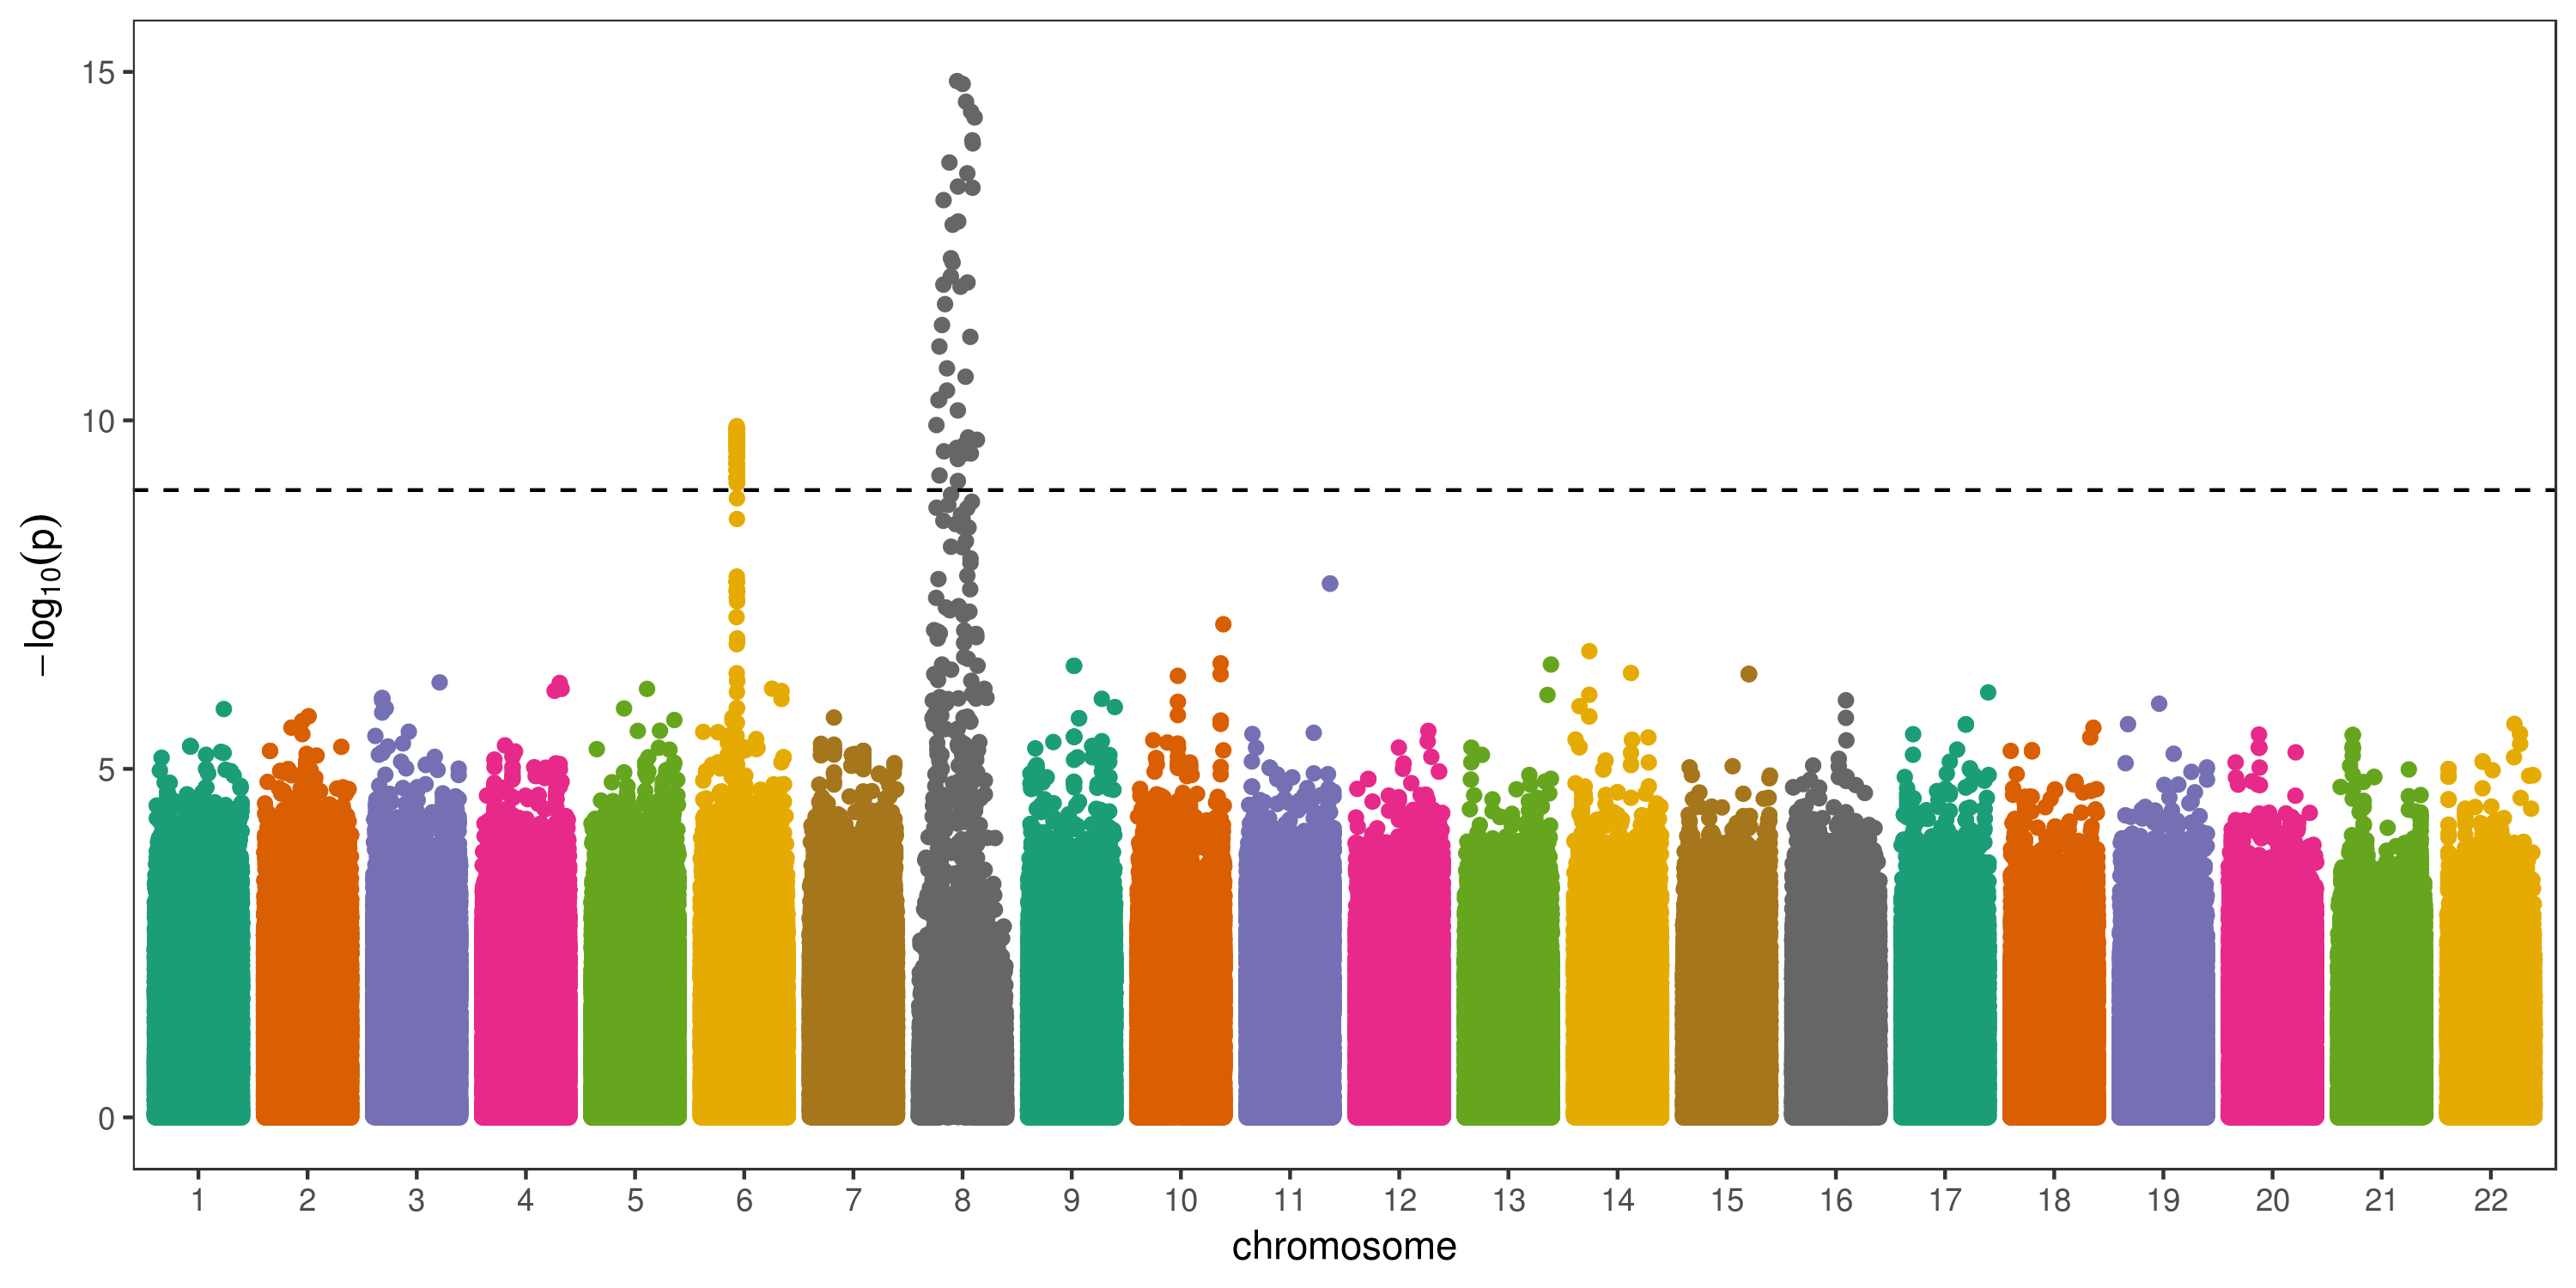
\includegraphics[width=\textwidth]{figs/fakepcs/beta2_2pcs_fake_manh}
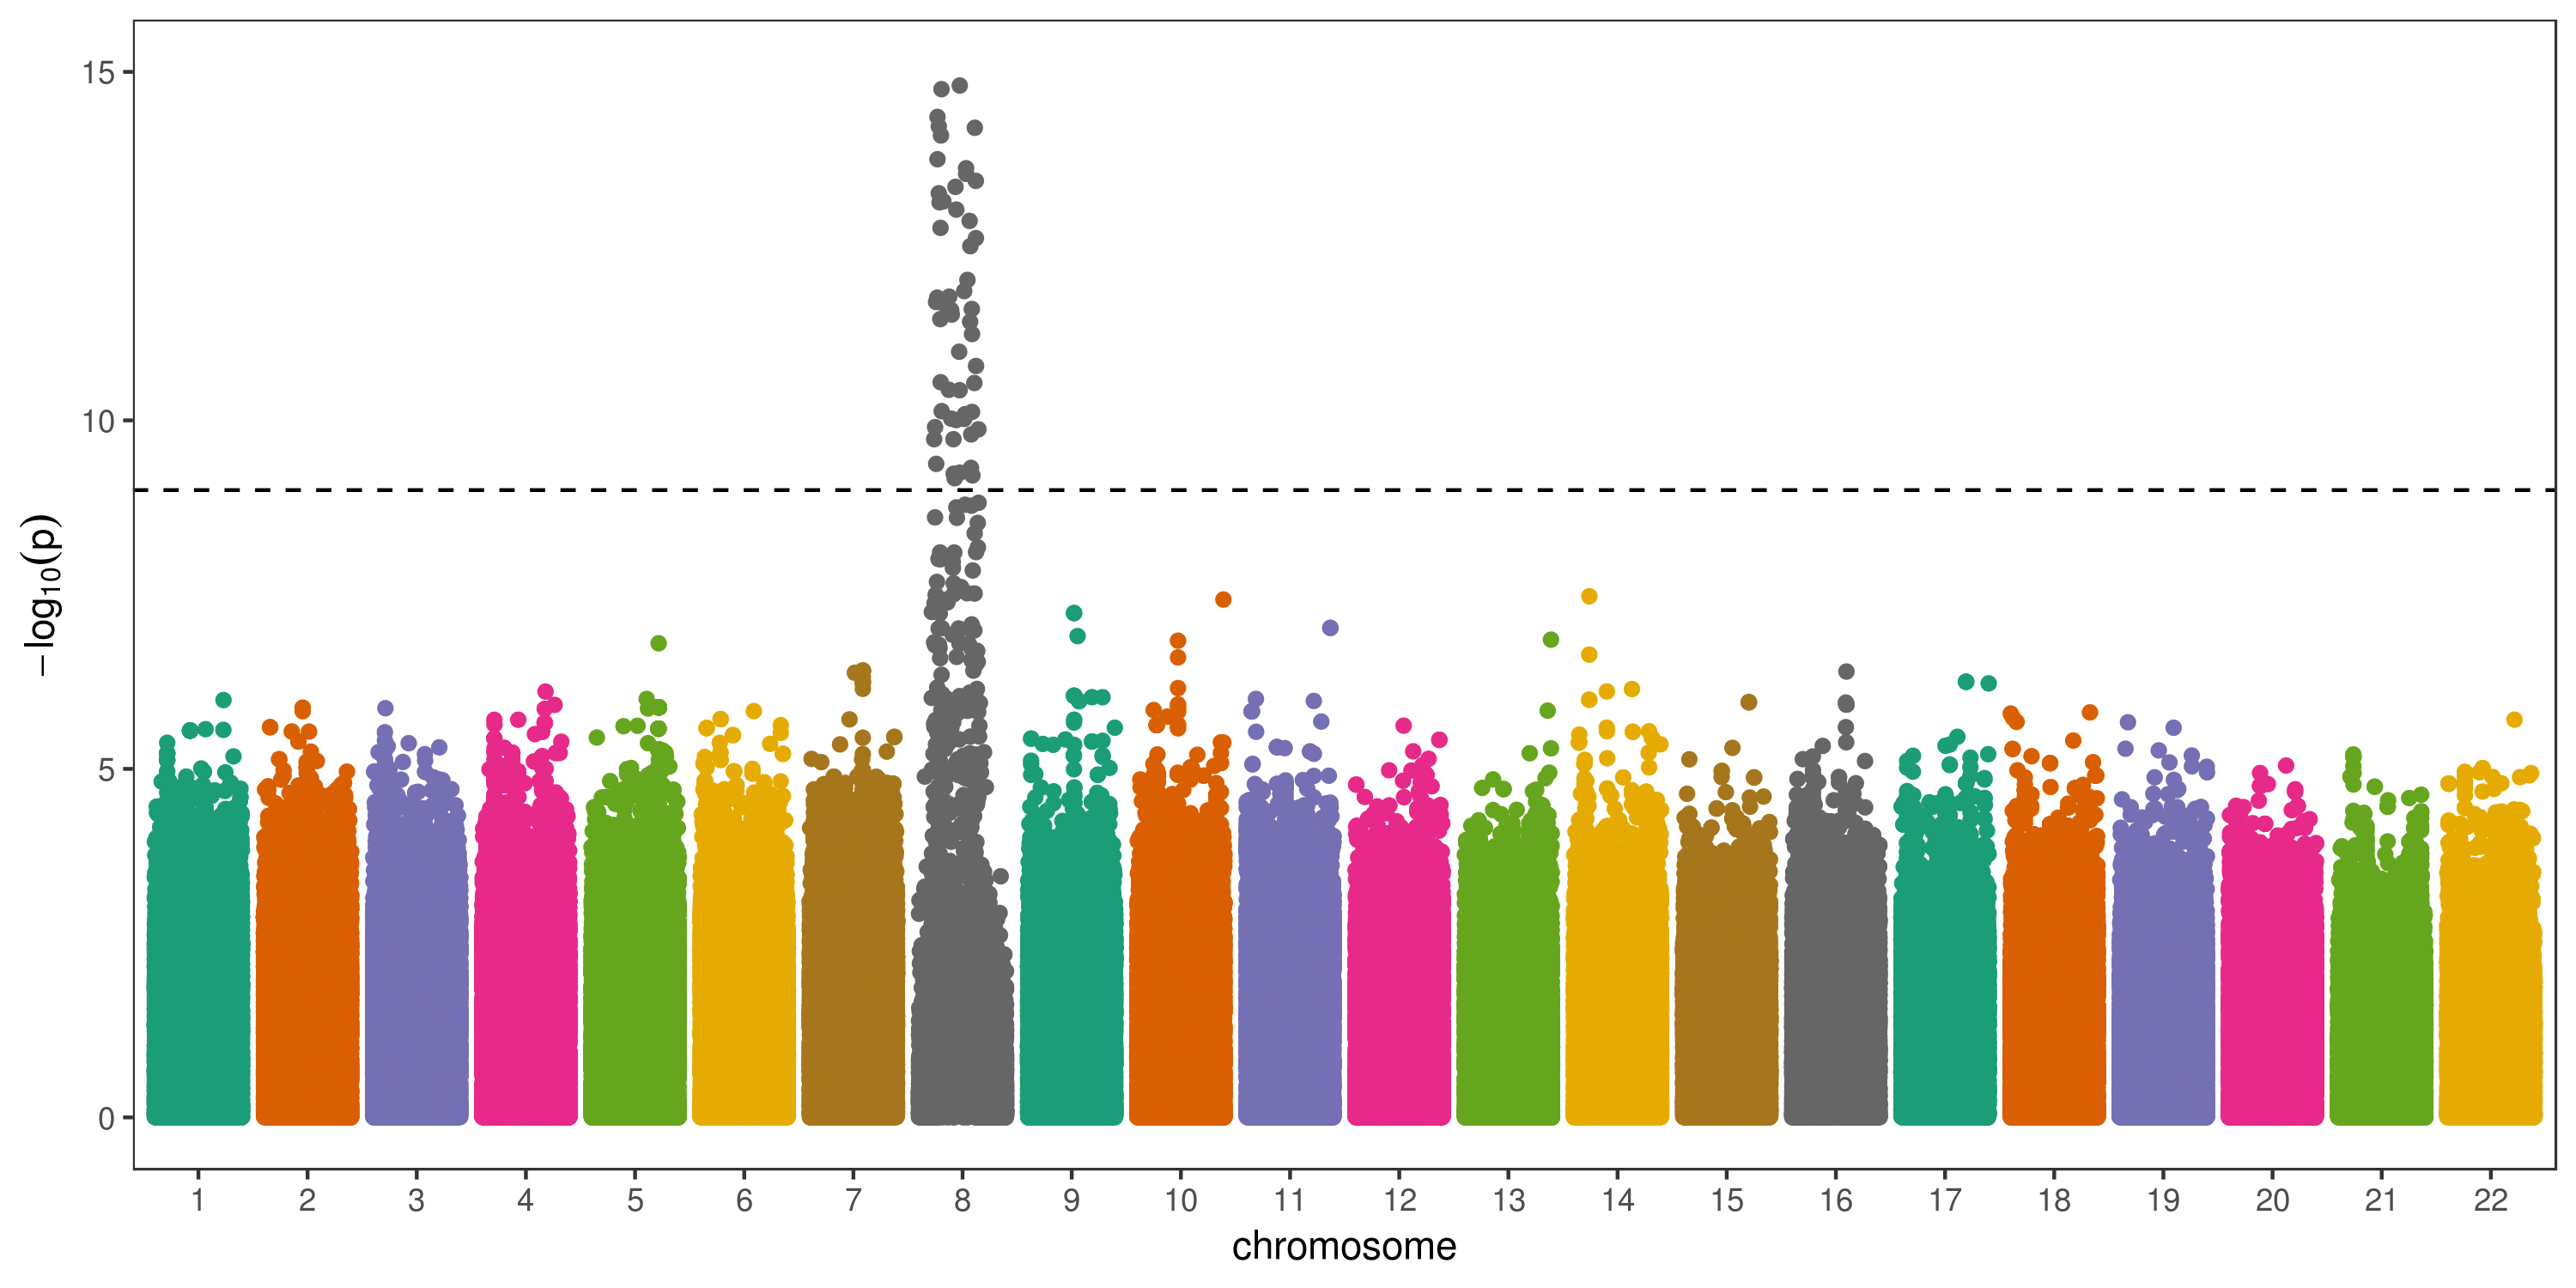
\includegraphics[width=\textwidth]{figs/finalfigs/figS12a_beta2_1pcs_fake_manh}
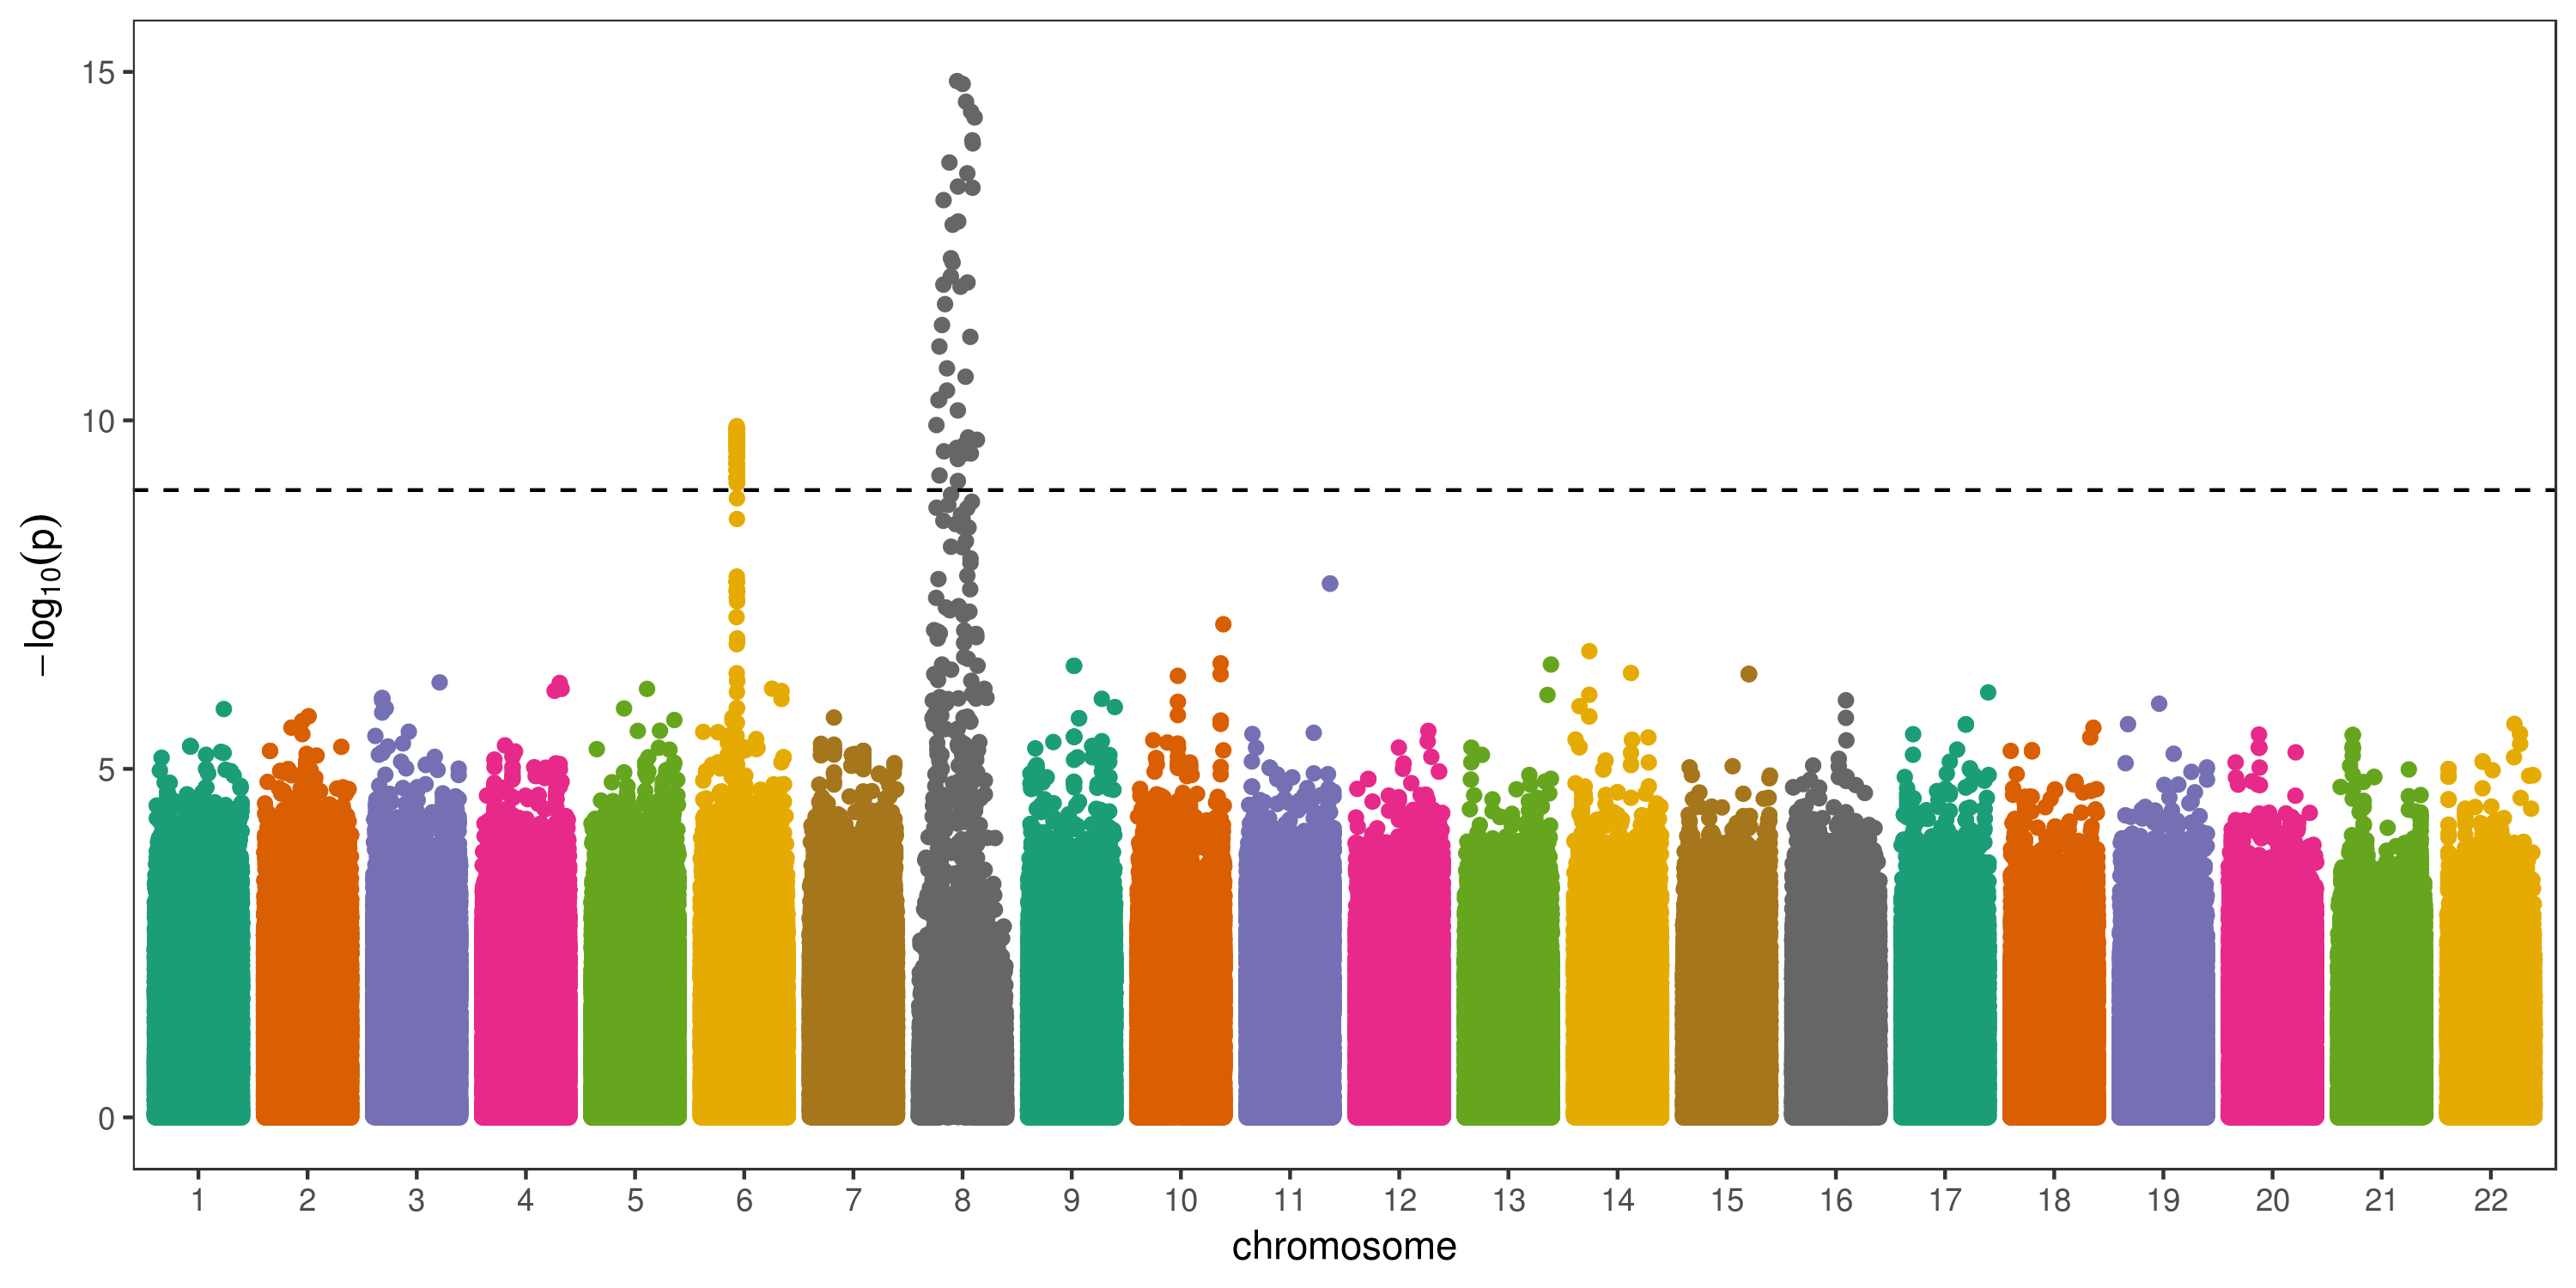
\includegraphics[width=\textwidth]{figs/finalfigs/figS12b_beta2_2pcs_fake_manh}
\caption[Manhattan plots for GWAS models adjusting for fake PCs in TOPMed JHS.]{Manhattan plots for GWAS models adjusting for fake PCs (i.e., PCs that were constructed such that the first captures genetic ancestry but the second captures genotype at two variants on chromosomes 6 and 8) in TOPMed JHS African Americans. The top panel presents results from a model adjusting for only the first PC and the bottom panel presents results from a model adjusting for two PCs. In this simulation setting, there is only one causal variant, located on chromosome 8.}
\label{fig:manh-fake}
\end{figure}

\begin{figure}[!htb]
\centering
%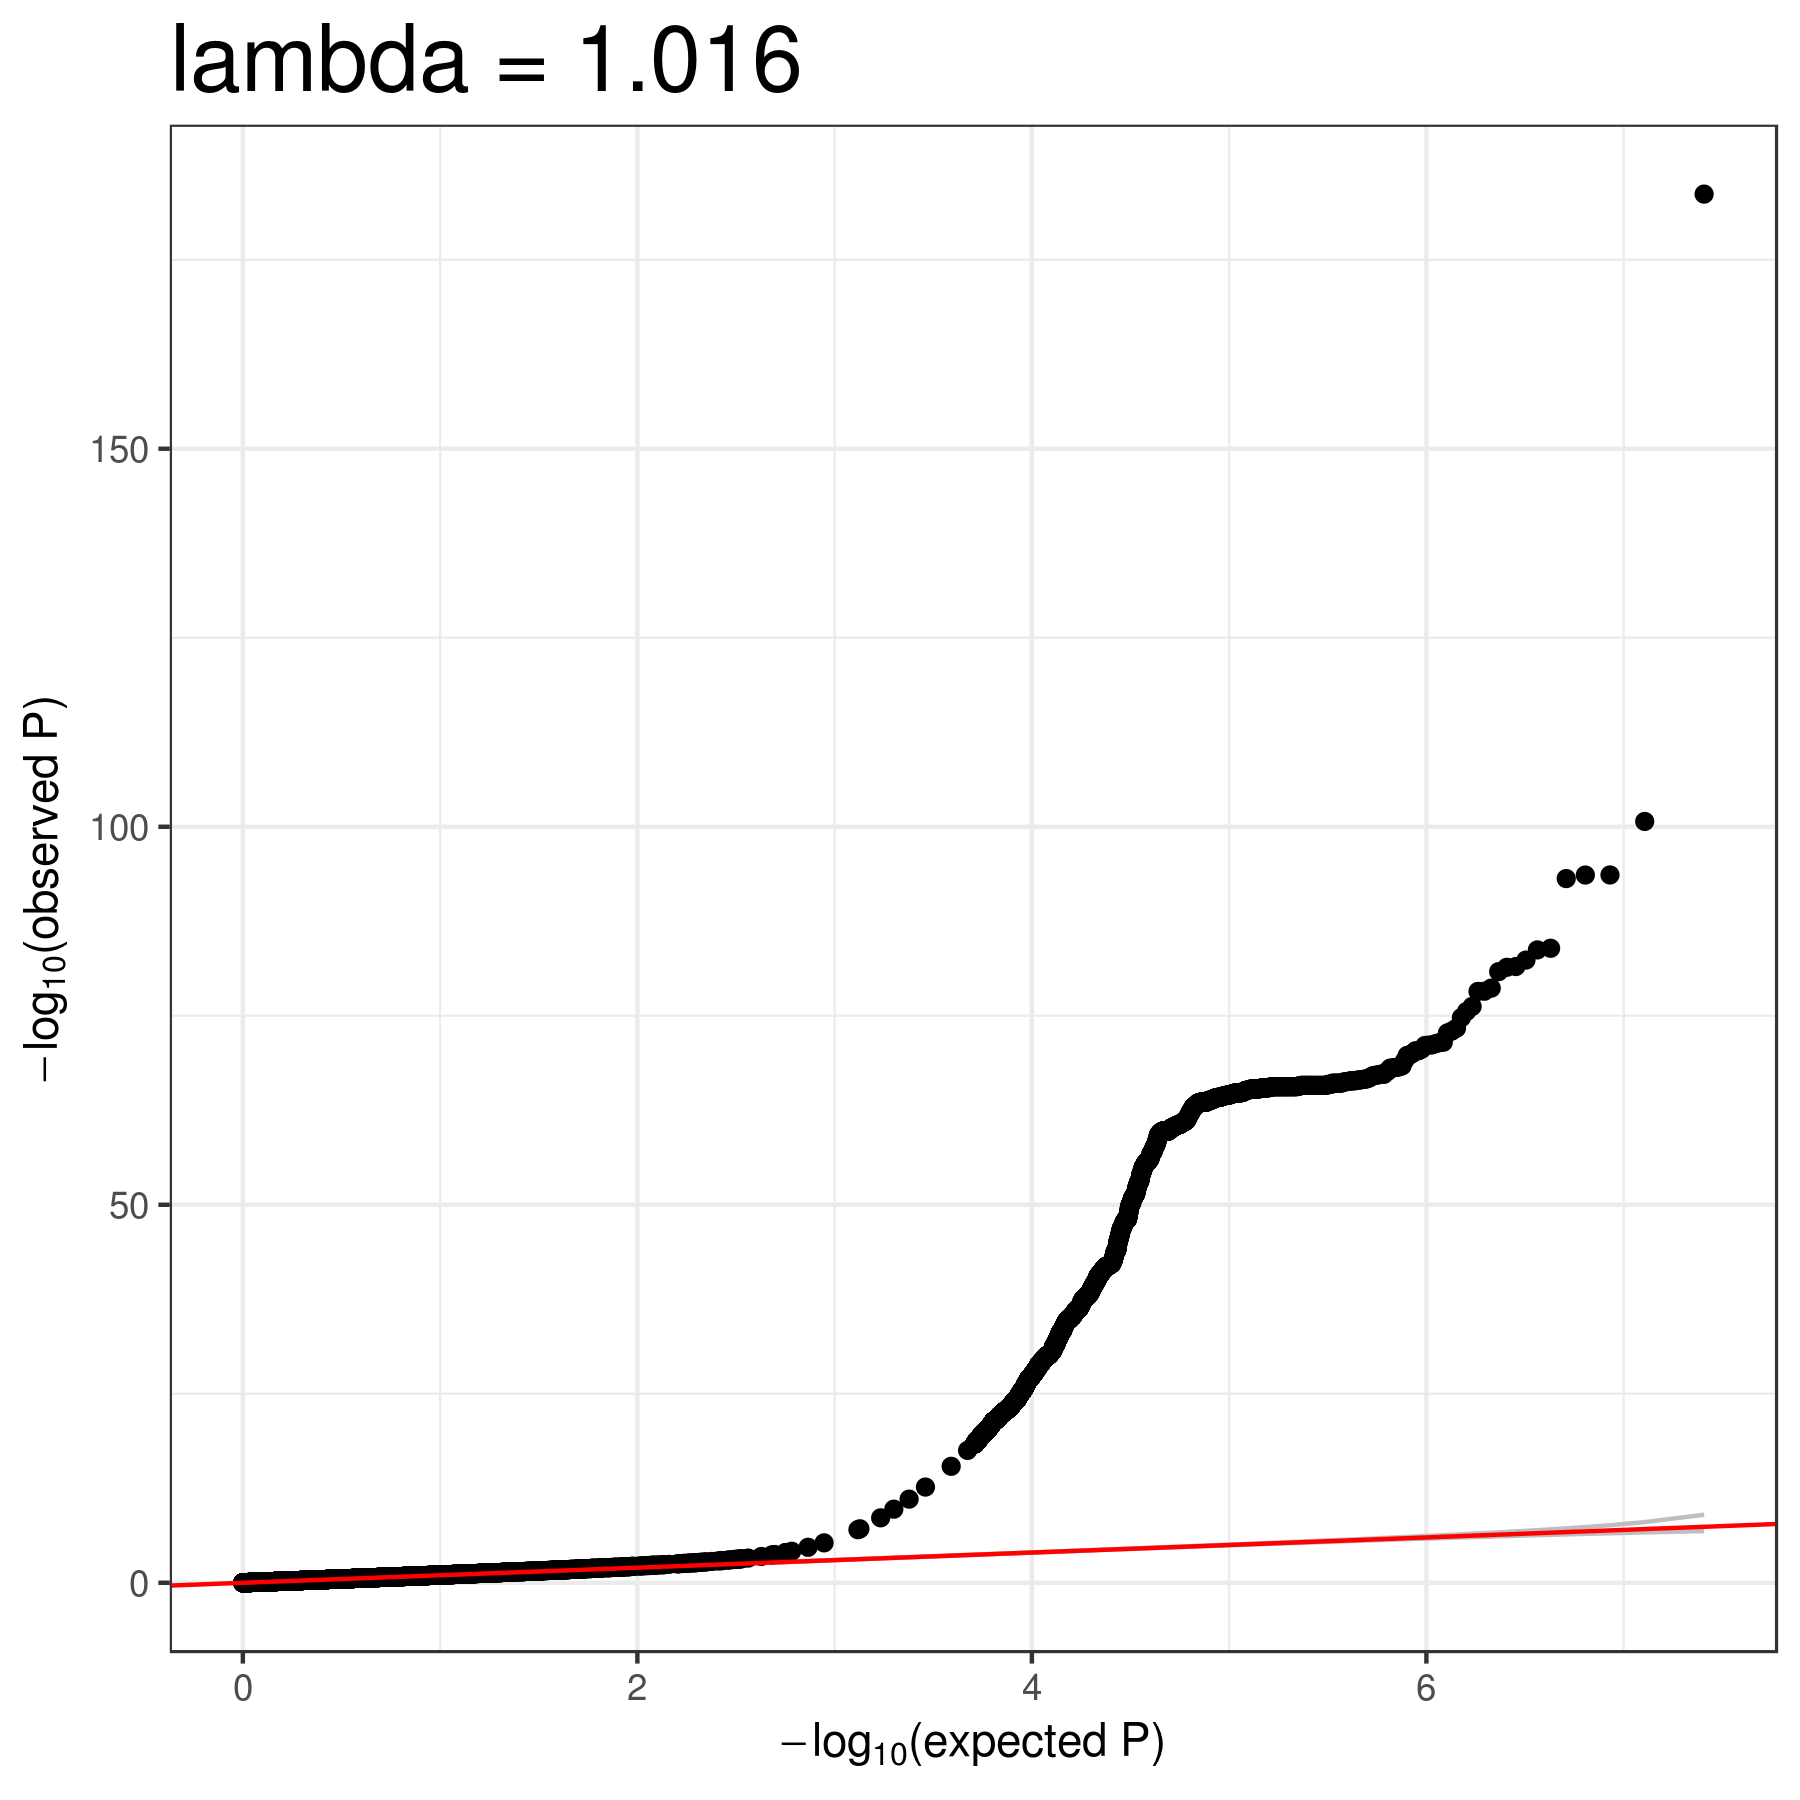
\includegraphics[width=0.48\textwidth]{figs/fakepcs/beta2_1pcs_fake_qq}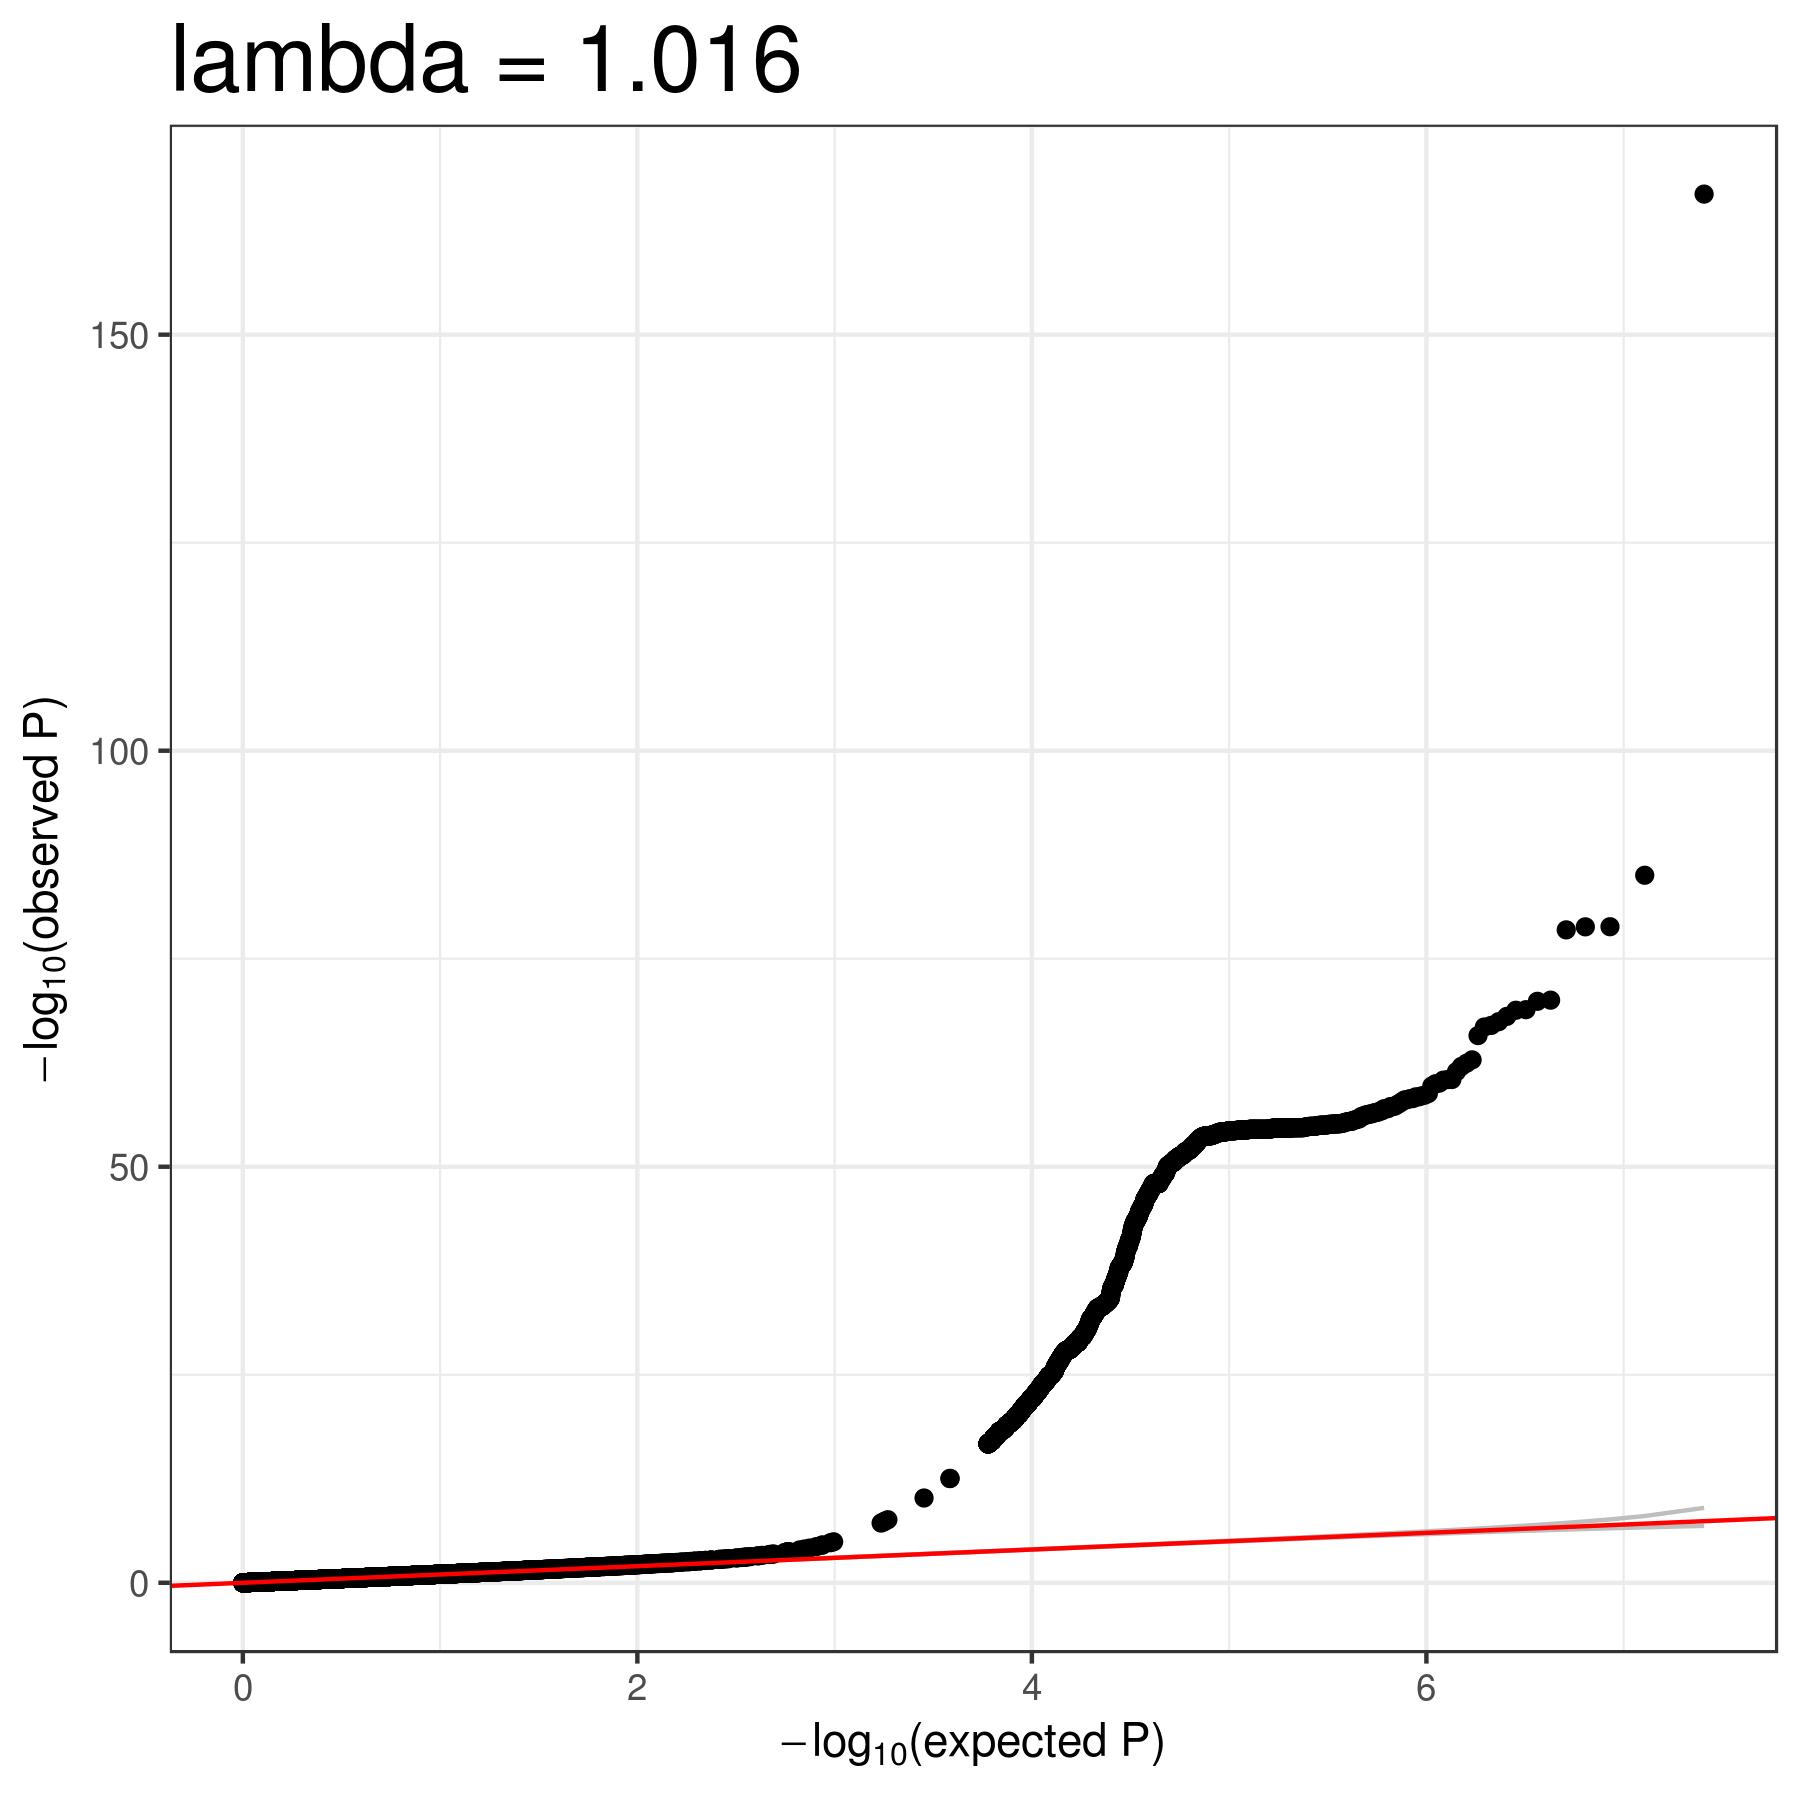
\includegraphics[width=0.48\textwidth]{figs/fakepcs/beta2_2pcs_fake_qq}
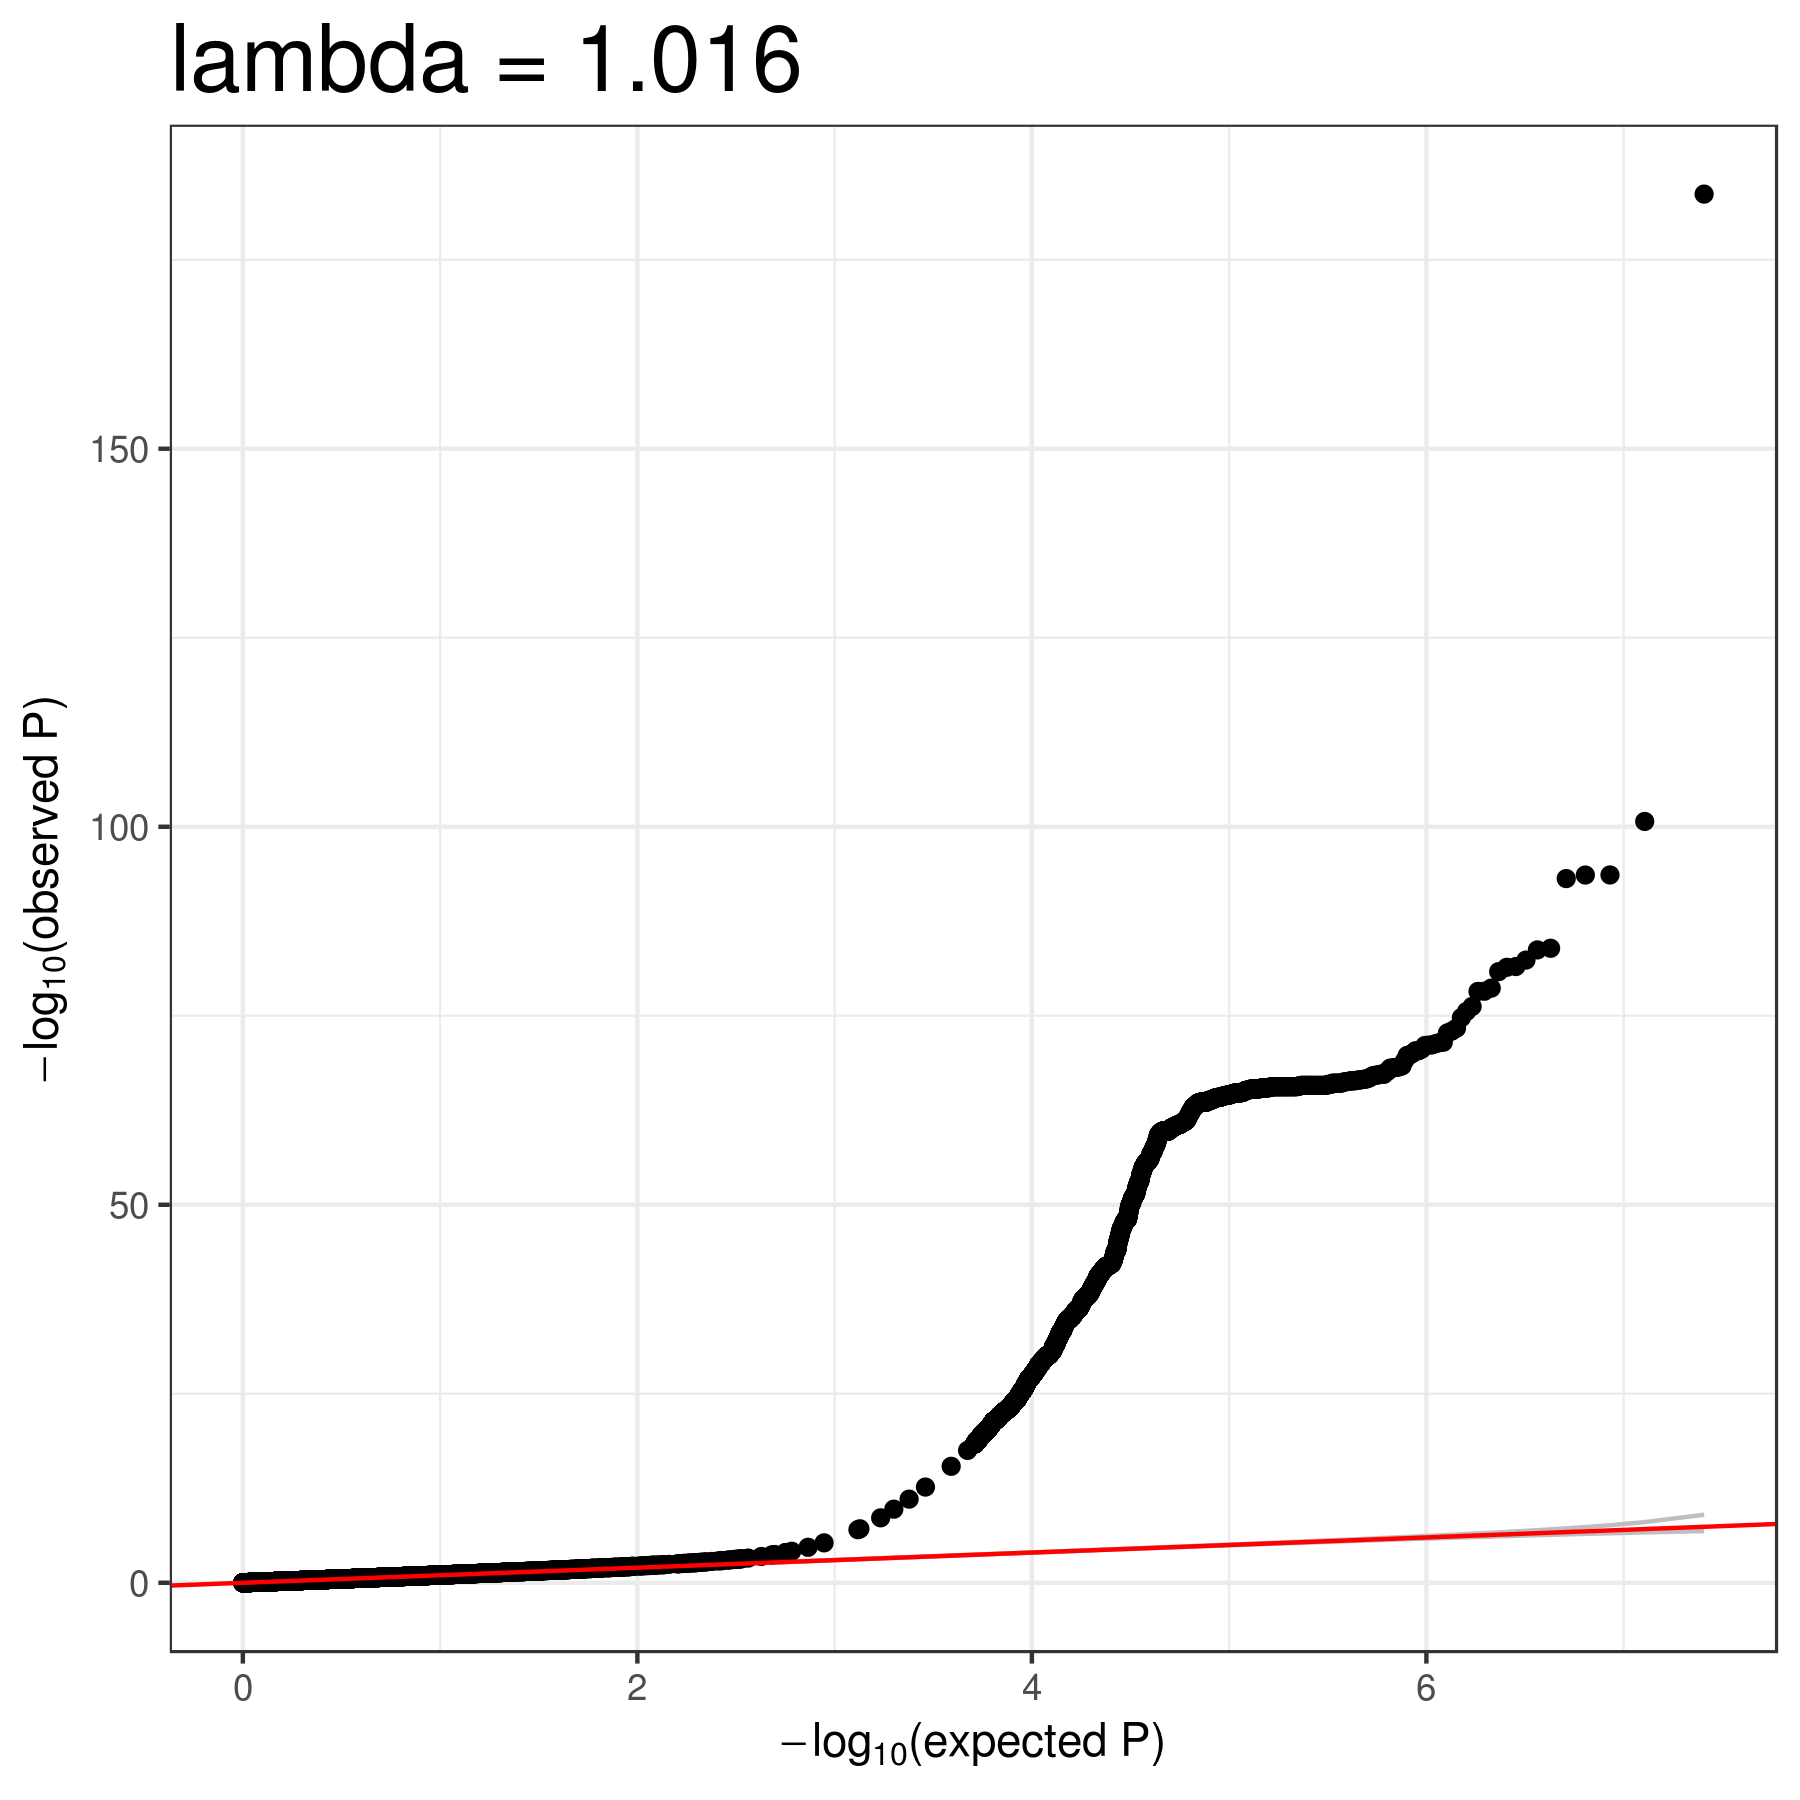
\includegraphics[width=0.48\textwidth]{figs/finalfigs/figS13a_beta2_1pcs_fake_qq}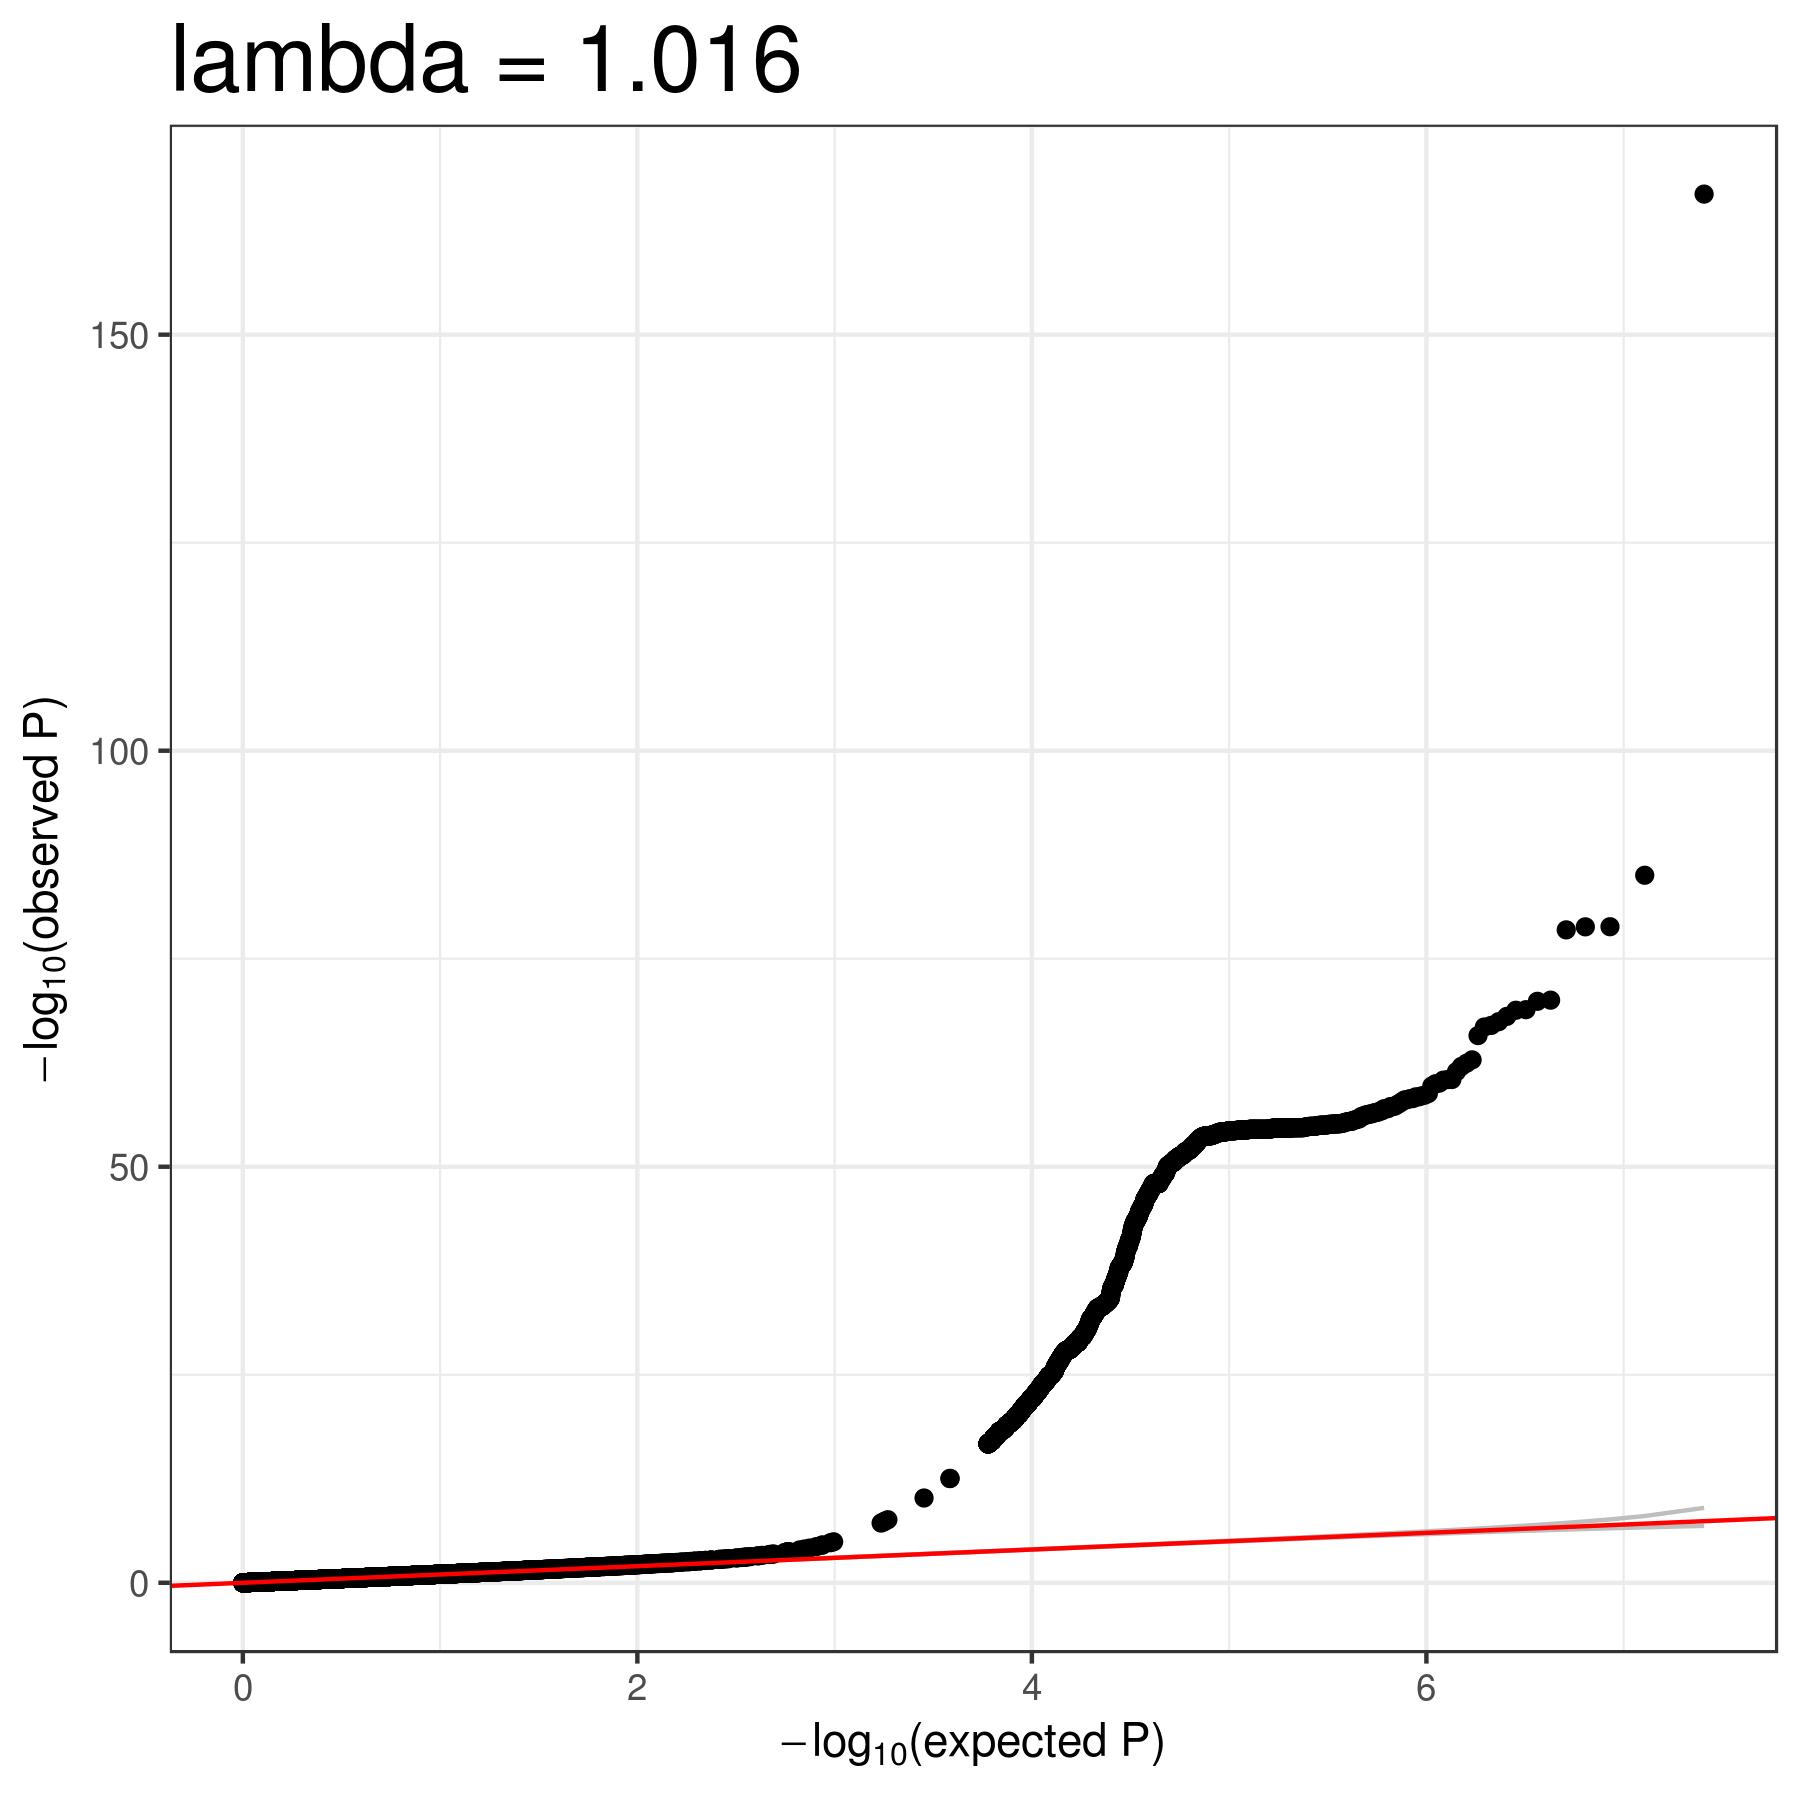
\includegraphics[width=0.48\textwidth]{figs/finalfigs/figS13b_beta2_2pcs_fake_qq}
\caption[QQ plots for GWAS models adjusting for fake PCs in TOPMed JHS.]{Quantile-quantile (QQ) plots and inflation factors ($\lambda$) for GWAS models adjusting for fake PCs (i.e., PCs that were constructed such that the first captures genetic ancestry but the second captures genotype at two variants on chromosomes 6 and 8) in TOPMed JHS African Americans. The left panel presents results from a model adjusting for only the first PC and the right panel presents results from a model adjusting for two PCs. The two plots are indistinguishable.}
\label{fig:qq-fake}
\end{figure}



\bibliographystyle{ajhg}
\bibliography{spurious}


\end{document}